% Options for packages loaded elsewhere
\PassOptionsToPackage{unicode}{hyperref}
\PassOptionsToPackage{hyphens}{url}
%
\documentclass[
]{book}
\usepackage{amsmath,amssymb}
\usepackage{lmodern}
\usepackage{iftex}
\ifPDFTeX
  \usepackage[T1]{fontenc}
  \usepackage[utf8]{inputenc}
  \usepackage{textcomp} % provide euro and other symbols
\else % if luatex or xetex
  \usepackage{unicode-math}
  \defaultfontfeatures{Scale=MatchLowercase}
  \defaultfontfeatures[\rmfamily]{Ligatures=TeX,Scale=1}
\fi
% Use upquote if available, for straight quotes in verbatim environments
\IfFileExists{upquote.sty}{\usepackage{upquote}}{}
\IfFileExists{microtype.sty}{% use microtype if available
  \usepackage[]{microtype}
  \UseMicrotypeSet[protrusion]{basicmath} % disable protrusion for tt fonts
}{}
\makeatletter
\@ifundefined{KOMAClassName}{% if non-KOMA class
  \IfFileExists{parskip.sty}{%
    \usepackage{parskip}
  }{% else
    \setlength{\parindent}{0pt}
    \setlength{\parskip}{6pt plus 2pt minus 1pt}}
}{% if KOMA class
  \KOMAoptions{parskip=half}}
\makeatother
\usepackage{xcolor}
\IfFileExists{xurl.sty}{\usepackage{xurl}}{} % add URL line breaks if available
\IfFileExists{bookmark.sty}{\usepackage{bookmark}}{\usepackage{hyperref}}
\hypersetup{
  pdftitle={庄闪闪的可视化手册},
  pdfauthor={庄亮亮},
  hidelinks,
  pdfcreator={LaTeX via pandoc}}
\urlstyle{same} % disable monospaced font for URLs
\usepackage{color}
\usepackage{fancyvrb}
\newcommand{\VerbBar}{|}
\newcommand{\VERB}{\Verb[commandchars=\\\{\}]}
\DefineVerbatimEnvironment{Highlighting}{Verbatim}{commandchars=\\\{\}}
% Add ',fontsize=\small' for more characters per line
\usepackage{framed}
\definecolor{shadecolor}{RGB}{248,248,248}
\newenvironment{Shaded}{\begin{snugshade}}{\end{snugshade}}
\newcommand{\AlertTok}[1]{\textcolor[rgb]{0.94,0.16,0.16}{#1}}
\newcommand{\AnnotationTok}[1]{\textcolor[rgb]{0.56,0.35,0.01}{\textbf{\textit{#1}}}}
\newcommand{\AttributeTok}[1]{\textcolor[rgb]{0.77,0.63,0.00}{#1}}
\newcommand{\BaseNTok}[1]{\textcolor[rgb]{0.00,0.00,0.81}{#1}}
\newcommand{\BuiltInTok}[1]{#1}
\newcommand{\CharTok}[1]{\textcolor[rgb]{0.31,0.60,0.02}{#1}}
\newcommand{\CommentTok}[1]{\textcolor[rgb]{0.56,0.35,0.01}{\textit{#1}}}
\newcommand{\CommentVarTok}[1]{\textcolor[rgb]{0.56,0.35,0.01}{\textbf{\textit{#1}}}}
\newcommand{\ConstantTok}[1]{\textcolor[rgb]{0.00,0.00,0.00}{#1}}
\newcommand{\ControlFlowTok}[1]{\textcolor[rgb]{0.13,0.29,0.53}{\textbf{#1}}}
\newcommand{\DataTypeTok}[1]{\textcolor[rgb]{0.13,0.29,0.53}{#1}}
\newcommand{\DecValTok}[1]{\textcolor[rgb]{0.00,0.00,0.81}{#1}}
\newcommand{\DocumentationTok}[1]{\textcolor[rgb]{0.56,0.35,0.01}{\textbf{\textit{#1}}}}
\newcommand{\ErrorTok}[1]{\textcolor[rgb]{0.64,0.00,0.00}{\textbf{#1}}}
\newcommand{\ExtensionTok}[1]{#1}
\newcommand{\FloatTok}[1]{\textcolor[rgb]{0.00,0.00,0.81}{#1}}
\newcommand{\FunctionTok}[1]{\textcolor[rgb]{0.00,0.00,0.00}{#1}}
\newcommand{\ImportTok}[1]{#1}
\newcommand{\InformationTok}[1]{\textcolor[rgb]{0.56,0.35,0.01}{\textbf{\textit{#1}}}}
\newcommand{\KeywordTok}[1]{\textcolor[rgb]{0.13,0.29,0.53}{\textbf{#1}}}
\newcommand{\NormalTok}[1]{#1}
\newcommand{\OperatorTok}[1]{\textcolor[rgb]{0.81,0.36,0.00}{\textbf{#1}}}
\newcommand{\OtherTok}[1]{\textcolor[rgb]{0.56,0.35,0.01}{#1}}
\newcommand{\PreprocessorTok}[1]{\textcolor[rgb]{0.56,0.35,0.01}{\textit{#1}}}
\newcommand{\RegionMarkerTok}[1]{#1}
\newcommand{\SpecialCharTok}[1]{\textcolor[rgb]{0.00,0.00,0.00}{#1}}
\newcommand{\SpecialStringTok}[1]{\textcolor[rgb]{0.31,0.60,0.02}{#1}}
\newcommand{\StringTok}[1]{\textcolor[rgb]{0.31,0.60,0.02}{#1}}
\newcommand{\VariableTok}[1]{\textcolor[rgb]{0.00,0.00,0.00}{#1}}
\newcommand{\VerbatimStringTok}[1]{\textcolor[rgb]{0.31,0.60,0.02}{#1}}
\newcommand{\WarningTok}[1]{\textcolor[rgb]{0.56,0.35,0.01}{\textbf{\textit{#1}}}}
\usepackage{longtable,booktabs,array}
\usepackage{calc} % for calculating minipage widths
% Correct order of tables after \paragraph or \subparagraph
\usepackage{etoolbox}
\makeatletter
\patchcmd\longtable{\par}{\if@noskipsec\mbox{}\fi\par}{}{}
\makeatother
% Allow footnotes in longtable head/foot
\IfFileExists{footnotehyper.sty}{\usepackage{footnotehyper}}{\usepackage{footnote}}
\makesavenoteenv{longtable}
\usepackage{graphicx}
\makeatletter
\def\maxwidth{\ifdim\Gin@nat@width>\linewidth\linewidth\else\Gin@nat@width\fi}
\def\maxheight{\ifdim\Gin@nat@height>\textheight\textheight\else\Gin@nat@height\fi}
\makeatother
% Scale images if necessary, so that they will not overflow the page
% margins by default, and it is still possible to overwrite the defaults
% using explicit options in \includegraphics[width, height, ...]{}
\setkeys{Gin}{width=\maxwidth,height=\maxheight,keepaspectratio}
% Set default figure placement to htbp
\makeatletter
\def\fps@figure{htbp}
\makeatother
\setlength{\emergencystretch}{3em} % prevent overfull lines
\providecommand{\tightlist}{%
  \setlength{\itemsep}{0pt}\setlength{\parskip}{0pt}}
\setcounter{secnumdepth}{5}
\usepackage{ctex}

%\usepackage{xltxtra} % XeLaTeX的一些额外符号
% 设置中文字体
%\setCJKmainfont[BoldFont={黑体},ItalicFont={楷体}]{新宋体}

% 设置边距
\usepackage{geometry}
\geometry{%
  left=2.0cm, right=2.0cm, top=3.5cm, bottom=2.5cm} 

\usepackage{amsthm,mathrsfs}
\usepackage{booktabs}
\usepackage{longtable}
\makeatletter
\def\thm@space@setup{%
  \thm@preskip=8pt plus 2pt minus 4pt
  \thm@postskip=\thm@preskip
}
\makeatother
\ifLuaTeX
  \usepackage{selnolig}  % disable illegal ligatures
\fi
\usepackage[style=apa,]{biblatex}
\addbibresource{mybib.bib}

\title{庄闪闪的可视化手册}
\author{庄亮亮}
\date{2022年2月5日}

\begin{document}
\maketitle

{
\setcounter{tocdepth}{1}
\tableofcontents
}
\hypertarget{ux7b80ux4ecb}{%
\chapter*{简介}\label{ux7b80ux4ecb}}
\addcontentsline{toc}{chapter}{简介}

R软件的bookdown扩展包是R Markdown的增强版,
支持自动目录、文献索引、公式编号与引用、定理编号与引用、图表自动编号与引用等功能,
可以作为LaTeX的一种替代解决方案,
在制作用R进行数据分析建模的技术报告时,
可以将报告文字、R程序、文字性结果、表格、图形都自动地融合在最后形成的网页或者PDF文件中。

Bookdown使用的设置比较复杂,
对初学者不够友好。
这里制作了一些模板,
用户只要解压缩打包的文件,
对某个模板进行修改填充就可以变成自己的中文图书或者论文。
Bookdown的详细用法参见\url{https://bookdown.org/yihui/bookdown/},
在李东风的\href{http://www.math.pku.edu.cn/teachers/lidf/docs/Rbook/html/_Rbook/index.html}{《统计软件教程》}也有部分介绍。

一些常用功能的示例在\texttt{0101-usage.Rmd}文件中,
用户可以在编辑器中打开此文件参考其中的做法。

Bookdown如果输出为网页,
其中的数学公式需要MathJax程序库的支持,
用如下数学公式测试浏览器中数学公式显示是否正常:

\[
\text{定积分} = \int_a^b f(x) \,dx
\]

如果显示不正常,
可以在公式上右键单击,
选择``Math Settings--Math Renderer'',
依次使用改成``Common HTML'',``SVG''等是否可以变成正常显示。
PDF版本不存在这样的问题。

\hypertarget{causal}{%
\chapter{基础包}\label{causal}}

\hypertarget{ux7ed8ux5236ux57faux672cux56feux5f62}{%
\section{绘制基本图形}\label{ux7ed8ux5236ux57faux672cux56feux5f62}}

\hypertarget{ux7ed8ux5236ux5206ux5e03ux5173ux7cfb}{%
\subsection{绘制分布关系}\label{ux7ed8ux5236ux5206ux5e03ux5173ux7cfb}}

数据的数字特征刻画了数据的主要特征,而对数据总体情况做全面描述时,研究人员需要研究数据的分布情况。

\textbf{主要方法}:绘制相应的图形,如直方图,条形图、饼图、箱线图等。

\hypertarget{ux76f4ux65b9ux56fe}{%
\subsubsection{直方图}\label{ux76f4ux65b9ux56fe}}

\textbf{概念介绍}:直方图(Histogram)由一系列高度不等的纵向条纹或者线段表示数据分布的情况。

\textbf{注意}:一般用横轴表示数据所属类别,纵轴表示数量或者占比。

\textbf{适用}:连续数据。

\textbf{例子}:我们使用模拟数据进行讲解,通过正态分布产生30个数据。

\begin{Shaded}
\begin{Highlighting}[]
\CommentTok{\# 数据模拟产生}
\NormalTok{x }\OtherTok{\textless{}{-}} \FunctionTok{rnorm}\NormalTok{(}\DecValTok{30}\NormalTok{, }\AttributeTok{mean =} \DecValTok{10}\NormalTok{, }\AttributeTok{sd =} \DecValTok{1}\NormalTok{)}
\FunctionTok{print}\NormalTok{(}\FunctionTok{round}\NormalTok{(x, }\DecValTok{2}\NormalTok{))}
\end{Highlighting}
\end{Shaded}

\begin{verbatim}
##  [1]  8.67 10.65  8.71  9.94  9.09 10.96 10.09  9.88 10.28 10.41 11.16  8.55
## [13] 10.62 11.19  9.82  9.85  9.89 10.81  9.73  9.60  8.58  9.83  9.61 10.55
## [25]  8.99 11.55  9.68 11.24  9.85  7.81
\end{verbatim}

\texttt{hist()}中的\texttt{breaks()}可以分段区间,取值可以是一个向量(各区间端点)或者一个数字(拆分为多少段),或者一个字符串(计算划分区间的算法名称),或者一个函数(划分区间个数的方法)。这里给出例子

\begin{Shaded}
\begin{Highlighting}[]
\FunctionTok{hist}\NormalTok{(x, }\AttributeTok{breaks =} \DecValTok{3}\NormalTok{)}
\end{Highlighting}
\end{Shaded}

\begin{center}\includegraphics{1001-chapter01_files/figure-latex/unnamed-chunk-3-1} \end{center}

\begin{Shaded}
\begin{Highlighting}[]
\FunctionTok{hist}\NormalTok{(x, }\AttributeTok{col =} \FunctionTok{rainbow}\NormalTok{(}\DecValTok{15}\NormalTok{), }\AttributeTok{breaks =} \DecValTok{3}\NormalTok{, }\AttributeTok{main =} \StringTok{"正态随机数"}\NormalTok{, }\AttributeTok{xlab =} \StringTok{""}\NormalTok{, }\AttributeTok{ylab =} \StringTok{"频数"}\NormalTok{)}
\end{Highlighting}
\end{Shaded}

\begin{center}\includegraphics{1001-chapter01_files/figure-latex/unnamed-chunk-3-2} \end{center}

\texttt{breaks\ =\ 3}表示x轴分为3个节点。其他设置可参考帮助文档,即\texttt{?hist}。这里加入其他参数\texttt{col,main,xlab,ylab},分别表示颜色,主题名称,x轴名称,y轴名称设置。细节将会在下面一章进行详细解释。

函数\texttt{density()}估计核密度。\texttt{freq=FALSE}绘制频率图。下面的程序作直方图,并使用\texttt{lines()}函数添加核密度曲线:

\begin{Shaded}
\begin{Highlighting}[]
\NormalTok{tmp.dens }\OtherTok{\textless{}{-}} \FunctionTok{density}\NormalTok{(x)}
\FunctionTok{hist}\NormalTok{(x, }\AttributeTok{freq =} \ConstantTok{FALSE}\NormalTok{, }\AttributeTok{ylim =} \FunctionTok{c}\NormalTok{(}\DecValTok{0}\NormalTok{, }\FunctionTok{max}\NormalTok{(tmp.dens}\SpecialCharTok{$}\NormalTok{y) }\SpecialCharTok{+} \FloatTok{0.1}\NormalTok{), }\AttributeTok{col =} \FunctionTok{rainbow}\NormalTok{(}\DecValTok{15}\NormalTok{), }\AttributeTok{main =} \StringTok{"正态随机数"}\NormalTok{, }
    \AttributeTok{xlab =} \StringTok{""}\NormalTok{, }\AttributeTok{ylab =} \StringTok{"频率"}\NormalTok{)}
\FunctionTok{lines}\NormalTok{(tmp.dens, }\AttributeTok{lwd =} \DecValTok{2}\NormalTok{, }\AttributeTok{col =} \StringTok{"blue"}\NormalTok{)}
\end{Highlighting}
\end{Shaded}

\begin{center}\includegraphics{1001-chapter01_files/figure-latex/unnamed-chunk-4-1} \end{center}

\hypertarget{ux6761ux5f62ux56fe}{%
\subsubsection{条形图}\label{ux6761ux5f62ux56fe}}

\textbf{概念介绍}:数量的多少画成长短不同的直条,然后把这些直条按一定的顺序排列起来。

\textbf{注意}:条形图的x轴是数据类别(\textbf{离散型}),y轴是相应类别的频数。

\begin{Shaded}
\begin{Highlighting}[]
\CommentTok{\# 复现课件中的条形图}
\NormalTok{gender }\OtherTok{=} \FunctionTok{table}\NormalTok{(}\FunctionTok{c}\NormalTok{(}\FunctionTok{rep}\NormalTok{(}\StringTok{"F"}\NormalTok{, }\DecValTok{12}\NormalTok{), }\FunctionTok{rep}\NormalTok{(}\StringTok{"M"}\NormalTok{, }\DecValTok{20}\NormalTok{)))}
\FunctionTok{barplot}\NormalTok{(gender, }\AttributeTok{col =} \FunctionTok{c}\NormalTok{(}\StringTok{"red"}\NormalTok{, }\StringTok{"green"}\NormalTok{), }\AttributeTok{main =} \StringTok{"性别分布"}\NormalTok{, }\AttributeTok{horiz =}\NormalTok{ T)}
\end{Highlighting}
\end{Shaded}

\begin{center}\includegraphics{1001-chapter01_files/figure-latex/unnamed-chunk-5-1} \end{center}

\textbf{数据介绍}:\texttt{VADeaths}数据集记录的是1940年Viginia(弗吉尼亚洲)不同人群(\texttt{Rural\ Male、Rural\ Female\ 、Urban\ Male、Urban\ Female})中每一千人的死亡情况。

\textbf{例子}:数据前6行展示如下:

\begin{tabular}{l|r|r|r|r}
\hline
  & Rural Male & Rural Female & Urban Male & Urban Female\\
\hline
50-54 & 11.7 & 8.7 & 15.4 & 8.4\\
\hline
55-59 & 18.1 & 11.7 & 24.3 & 13.6\\
\hline
60-64 & 26.9 & 20.3 & 37.0 & 19.3\\
\hline
65-69 & 41.0 & 30.9 & 54.6 & 35.1\\
\hline
70-74 & 66.0 & 54.3 & 71.1 & 50.0\\
\hline
\end{tabular}

这里绘制该数据的条形图。\texttt{beside}默认值为FALSE,每一列都将给出堆砌的``子条''高度,若 \texttt{beside=TRUE},则每一列都表示一个分组并列

\begin{Shaded}
\begin{Highlighting}[]
\FunctionTok{barplot}\NormalTok{(VADeaths)}
\end{Highlighting}
\end{Shaded}

\begin{center}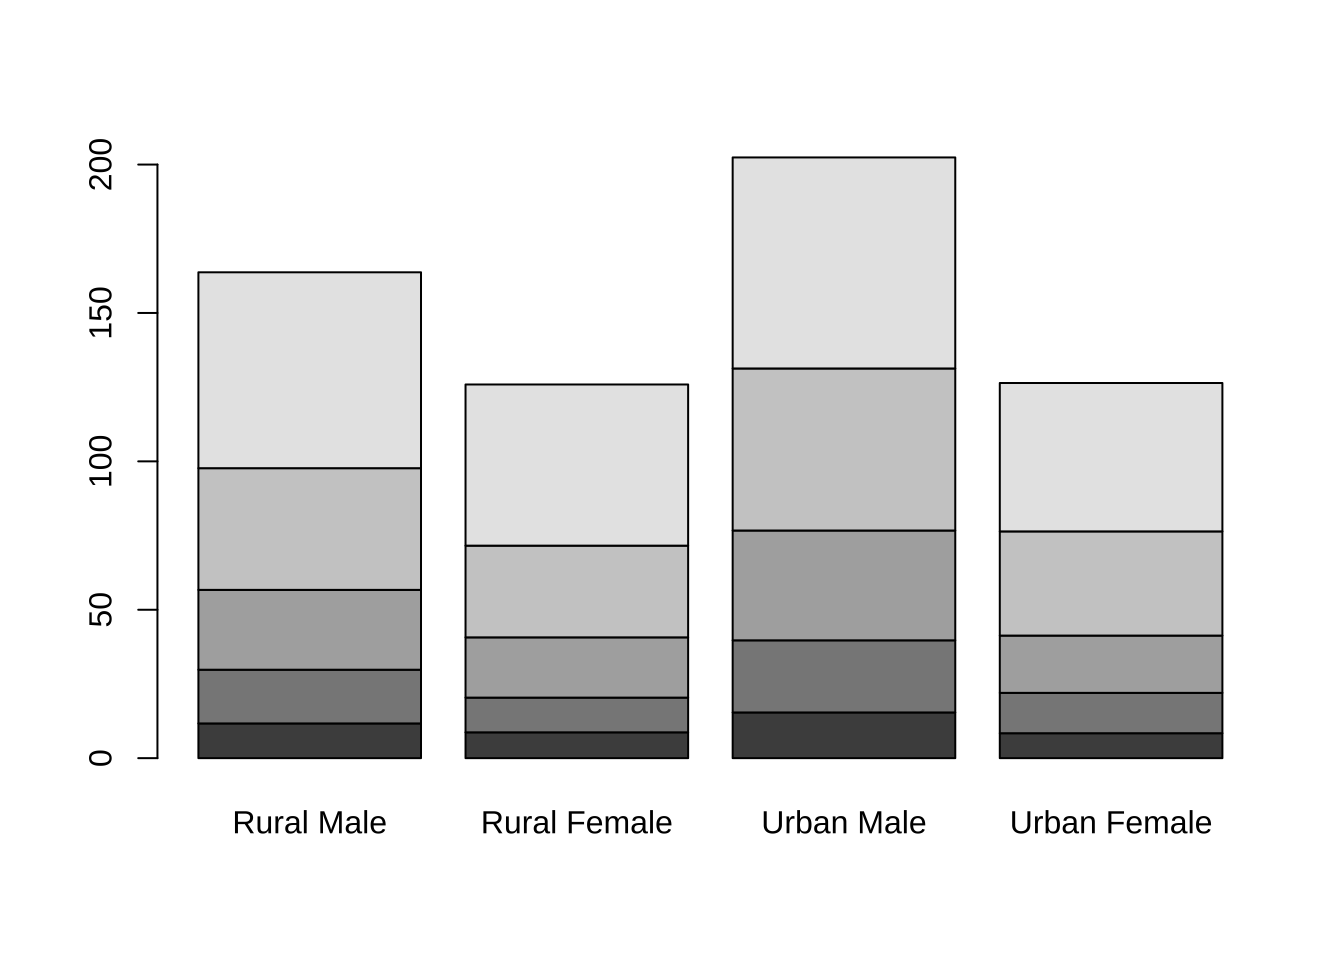
\includegraphics{1001-chapter01_files/figure-latex/unnamed-chunk-7-1} \end{center}

\begin{Shaded}
\begin{Highlighting}[]
\FunctionTok{barplot}\NormalTok{(VADeaths, }\AttributeTok{beside =} \ConstantTok{TRUE}\NormalTok{)}
\end{Highlighting}
\end{Shaded}

\begin{center}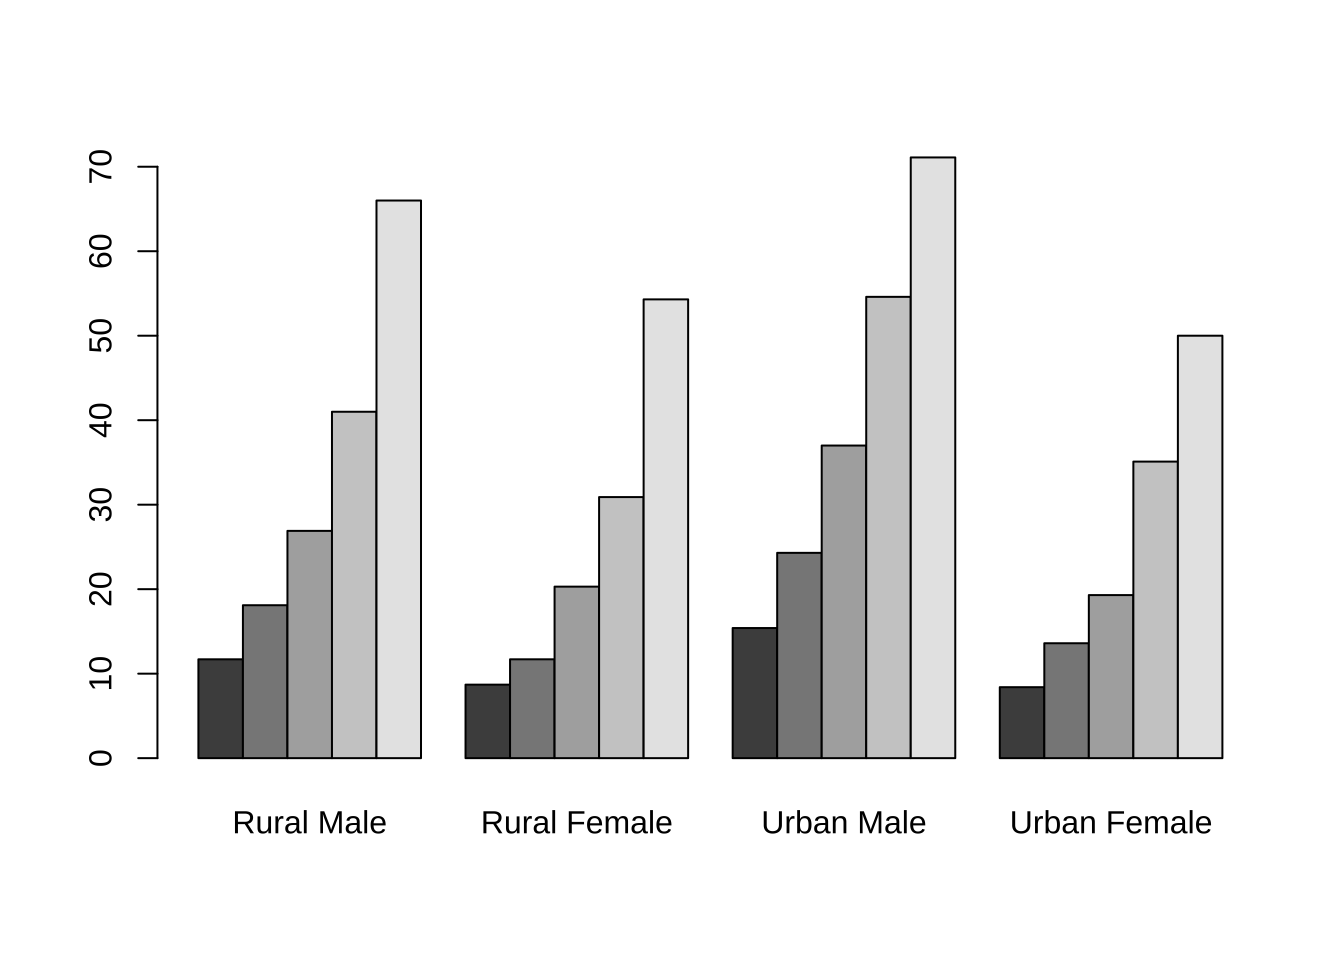
\includegraphics{1001-chapter01_files/figure-latex/unnamed-chunk-7-2} \end{center}

\textbf{结论:}随着年龄的增长,\texttt{Viginia}人群的死亡率逐渐增加,并且在4类人群中, \texttt{Urban\ Male}的死亡率比同年龄段的其他群体的死亡率高。同时,在同一环境下,相同年龄段的男性的死亡率要比女性高。

\hypertarget{ux997cux56fe}{%
\subsubsection{饼图}\label{ux997cux56fe}}

\textbf{概念介绍}:将各项的大小与各项总和的比例。反映部分与部分、部分与整体之间的比例关系。

\textbf{例子}:

\begin{Shaded}
\begin{Highlighting}[]
\NormalTok{percent }\OtherTok{\textless{}{-}} \FunctionTok{colSums}\NormalTok{(VADeaths) }\SpecialCharTok{*} \DecValTok{100}\SpecialCharTok{/}\FunctionTok{sum}\NormalTok{(VADeaths)}
\FunctionTok{pie}\NormalTok{(percent, }\AttributeTok{labels =} \FunctionTok{paste0}\NormalTok{(}\FunctionTok{colnames}\NormalTok{(VADeaths), }\StringTok{"}\SpecialCharTok{\textbackslash{}n}\StringTok{"}\NormalTok{, }\FunctionTok{round}\NormalTok{(percent, }\DecValTok{2}\NormalTok{), }\StringTok{"\%"}\NormalTok{))}
\end{Highlighting}
\end{Shaded}

\begin{center}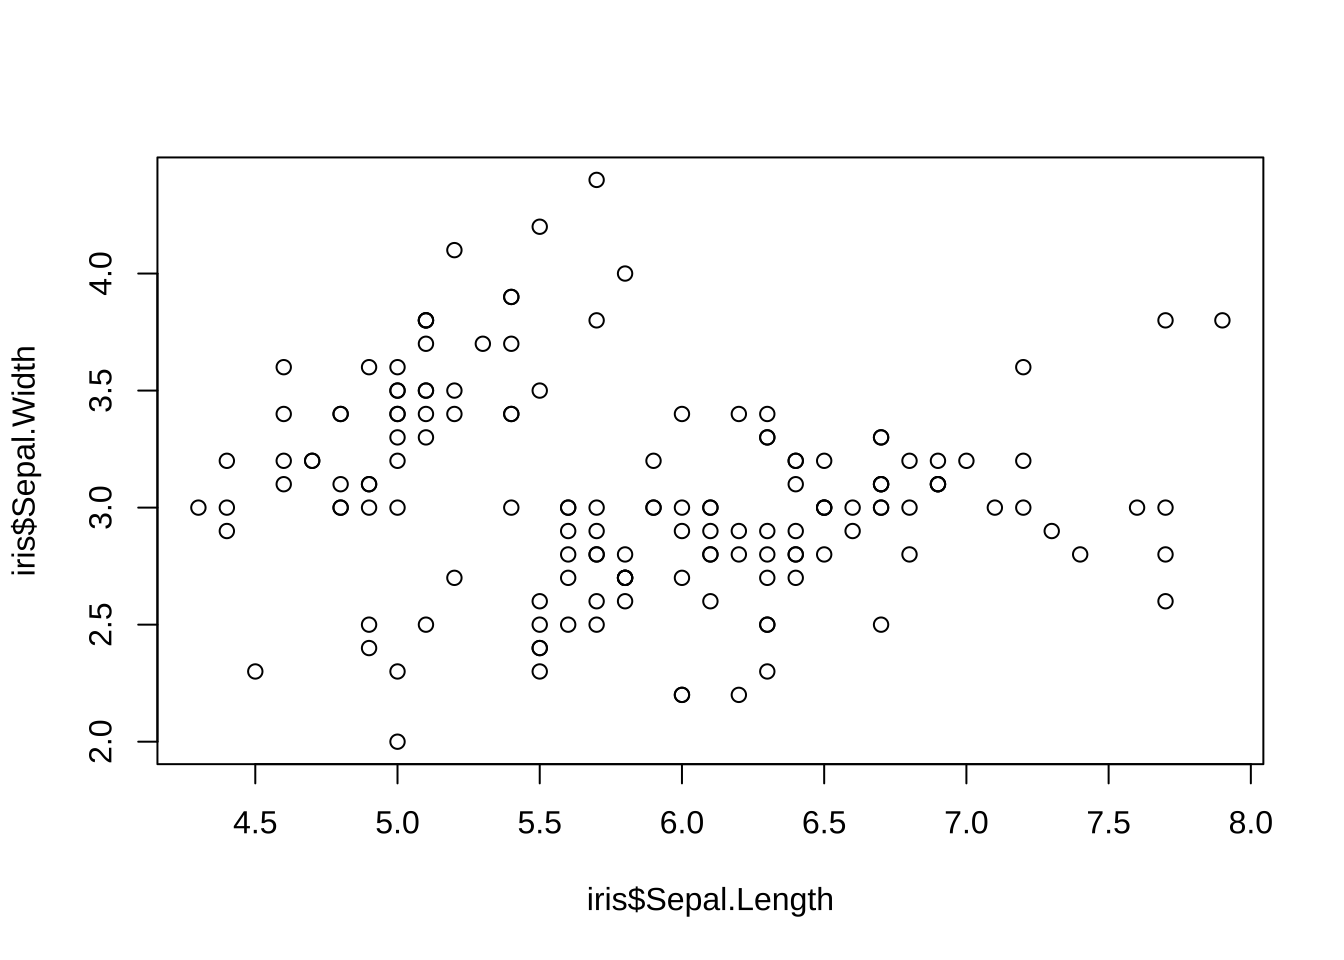
\includegraphics{1001-chapter01_files/figure-latex/unnamed-chunk-8-1} \end{center}

\begin{Shaded}
\begin{Highlighting}[]
\FunctionTok{pie}\NormalTok{(percent, }\AttributeTok{radius =} \FloatTok{0.8}\NormalTok{)  }\CommentTok{\#init.angle}
\end{Highlighting}
\end{Shaded}

\begin{center}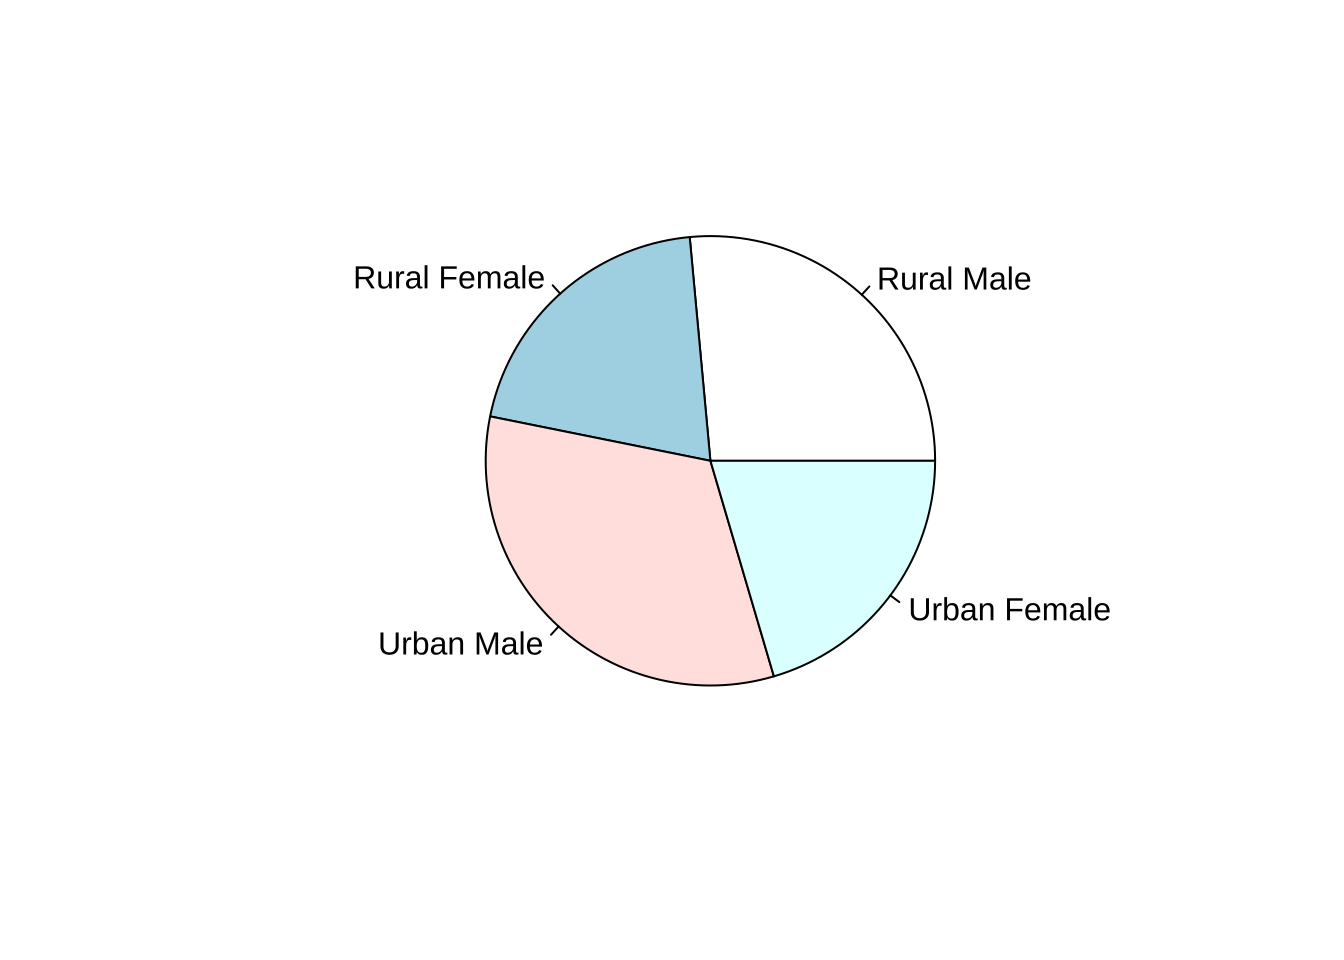
\includegraphics{1001-chapter01_files/figure-latex/unnamed-chunk-8-2} \end{center}

\begin{Shaded}
\begin{Highlighting}[]
\CommentTok{\# ?pie}
\end{Highlighting}
\end{Shaded}

\textbf{结论:}Virginia人群中死亡最高的是Urban Male,而且男性的死亡率比女性死亡率要高。

\hypertarget{ux7bb1ux7ebfux56fe}{%
\subsubsection{箱线图}\label{ux7bb1ux7ebfux56fe}}

\textbf{概念介绍}:绘制须使用常用的统计量(最小值、下四分位数、中位数、上四分位数和最大值),并提供有关数据位置和分散情况的关键信息,尤其在比较不同特征时,更可表现其分散程度差异。

\textbf{数据介绍}:iris数据集(鸢尾花数据集),是常用的分类实验数据集合,由Fisher在1936年收集整理。数据集包含了150个子数据集,分为3类(分别为setosa、versicolor、virginica),每类50个数据,每个数据包含4个属性,即花萼长度Sepal.Length 、花萼宽度Sepal.Width、花瓣长度Petal.Length、花瓣宽度Petal.Width。

前6行数据如下:

\begin{tabular}{r|r|r|r|l}
\hline
Sepal.Length & Sepal.Width & Petal.Length & Petal.Width & Species\\
\hline
5.1 & 3.5 & 1.4 & 0.2 & setosa\\
\hline
4.9 & 3.0 & 1.4 & 0.2 & setosa\\
\hline
4.7 & 3.2 & 1.3 & 0.2 & setosa\\
\hline
4.6 & 3.1 & 1.5 & 0.2 & setosa\\
\hline
5.0 & 3.6 & 1.4 & 0.2 & setosa\\
\hline
5.4 & 3.9 & 1.7 & 0.4 & setosa\\
\hline
\end{tabular}

\textbf{例子}:
使用箱线图进行分析,使用两种方法:单独分析四个变量内部的数据分布情况;组间比较(Sepal.Length \textasciitilde{} Species)注意这里的x应该是因子型。这里没有对其他参数进行添加,大家根据自己需求添加即可。

\begin{Shaded}
\begin{Highlighting}[]
\FunctionTok{attach}\NormalTok{(iris)}
\FunctionTok{boxplot}\NormalTok{(iris[}\DecValTok{1}\SpecialCharTok{:}\DecValTok{4}\NormalTok{], }\AttributeTok{main =} \StringTok{"单独的箱线图"}\NormalTok{)}
\end{Highlighting}
\end{Shaded}

\begin{center}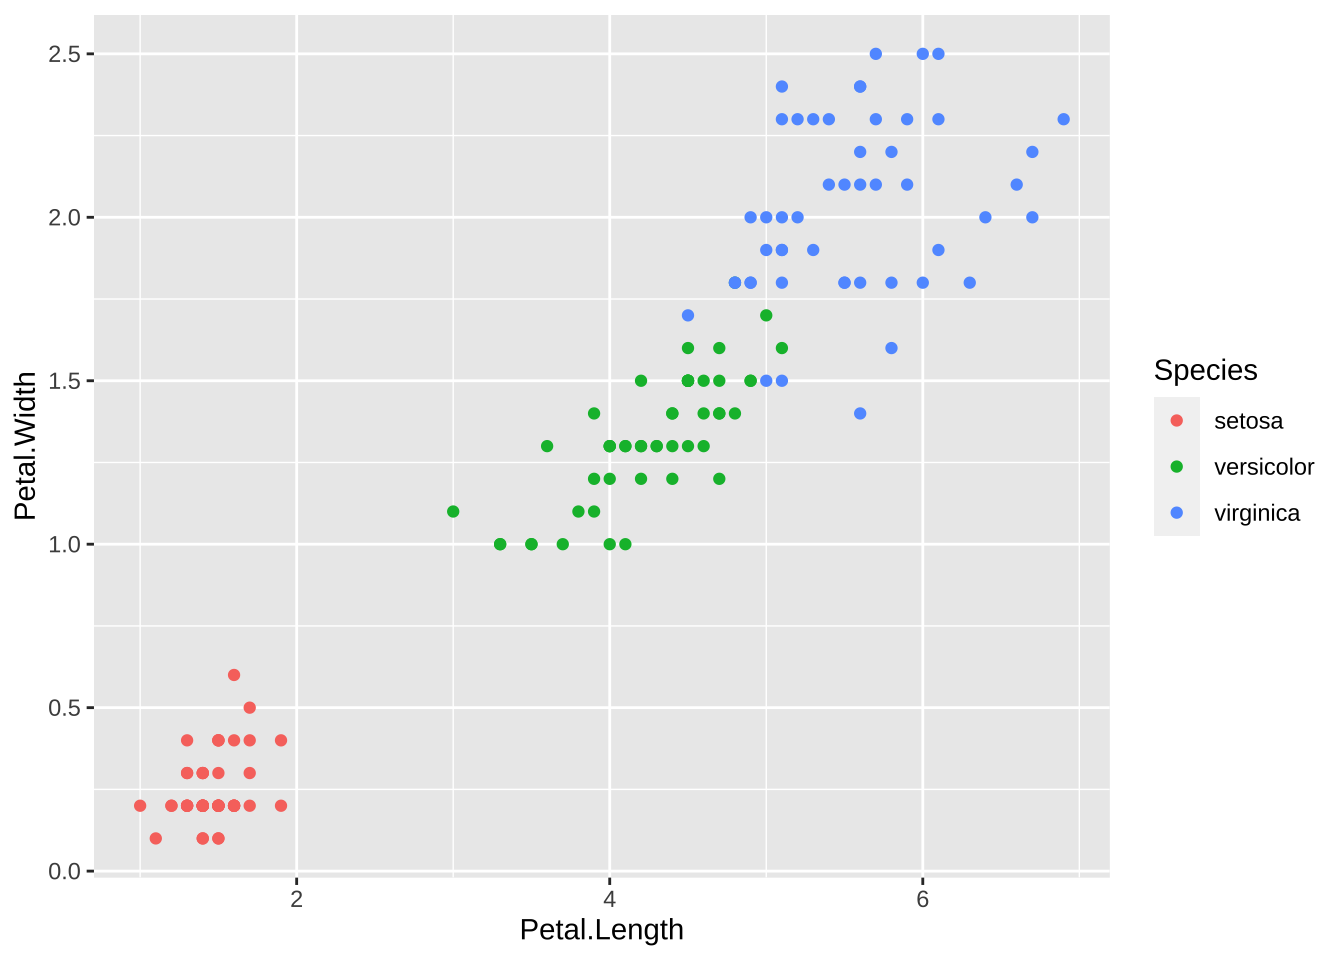
\includegraphics{1001-chapter01_files/figure-latex/unnamed-chunk-10-1} \end{center}

\begin{Shaded}
\begin{Highlighting}[]
\FunctionTok{boxplot}\NormalTok{(Sepal.Length }\SpecialCharTok{\textasciitilde{}}\NormalTok{ Species, }\AttributeTok{data =}\NormalTok{ iris, }\AttributeTok{main =} \StringTok{"组间比较的箱线图"}\NormalTok{)}
\end{Highlighting}
\end{Shaded}

\begin{center}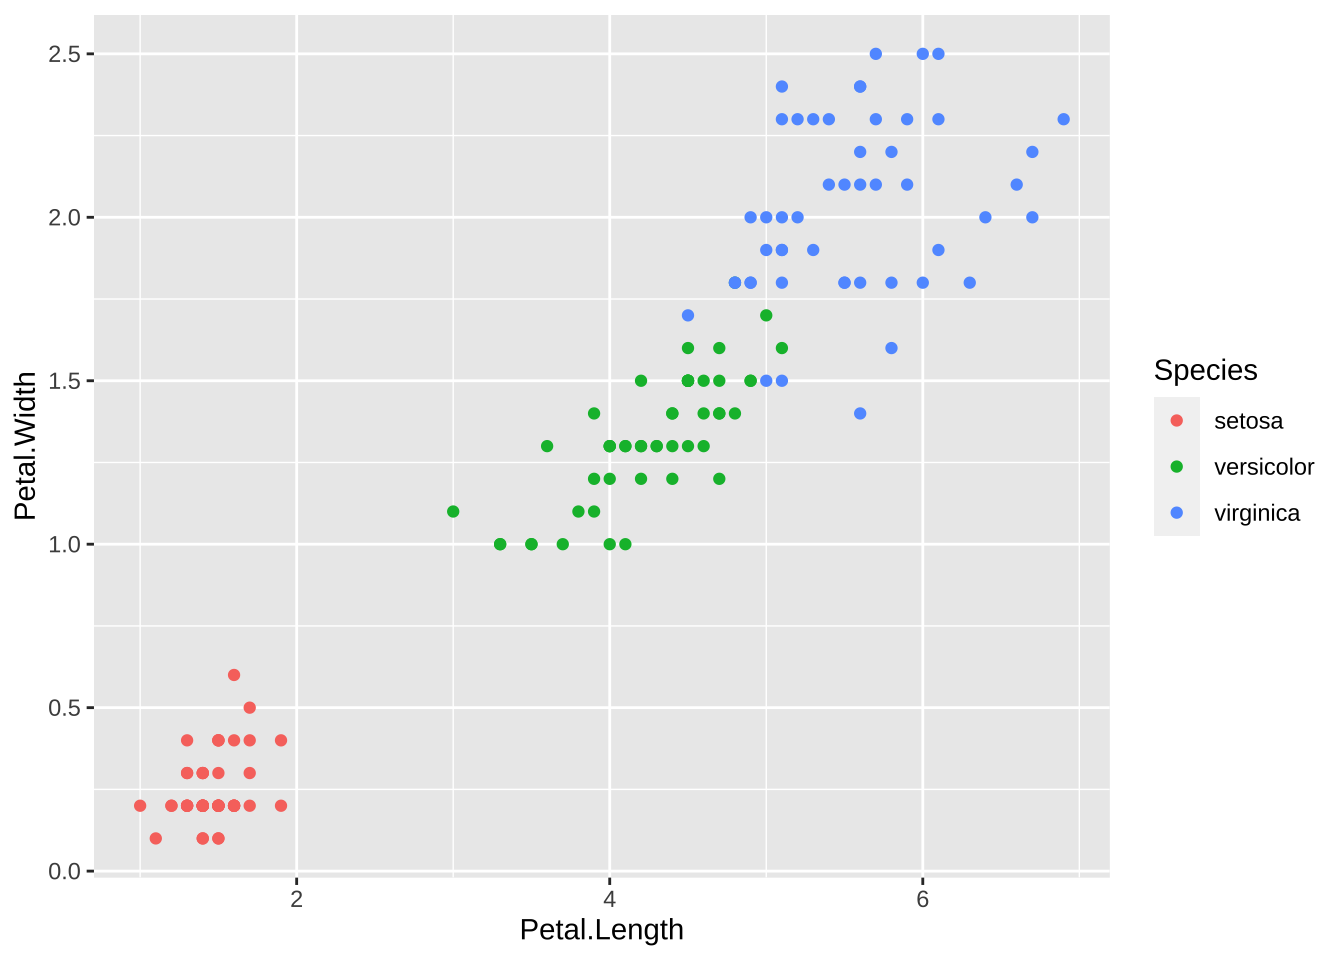
\includegraphics{1001-chapter01_files/figure-latex/unnamed-chunk-10-2} \end{center}

\textbf{结论:}第一个图:Sepal.Width列含有四个异常值。

第二个图:Sepal.Length列中,类别属于virginica的数据含有一个异常值。同时,从第一个图可以看到,Petal.Length列前半部分相对分散,而后半部分相对密集。

\hypertarget{ux7ed8ux5236ux6570ux636eux95f4ux5173ux7cfb}{%
\subsection{绘制数据间关系}\label{ux7ed8ux5236ux6570ux636eux95f4ux5173ux7cfb}}

\textbf{概念介绍}:在分析数据间关系时,常用散点图和多变量相关矩阵图查看数据间的相关关系。

\hypertarget{ux6563ux70b9ux56fe}{%
\subsubsection{散点图}\label{ux6563ux70b9ux56fe}}

\textbf{特点:}

\begin{enumerate}
\def\labelenumi{(\arabic{enumi})}
\item
  特征之间是否存在关联趋势,关联趋势是线性的还是非线性的。
\item
  一目了然的看出离群值。从而可以进一步分析这些离群值是否可能在建模分析中产生很大的影响。
\end{enumerate}

\textbf{例子}:使用cars数据进行分析速度(speed)和刹车距离(dist)之间的关系

\begin{Shaded}
\begin{Highlighting}[]
\FunctionTok{plot}\NormalTok{(cars[, }\DecValTok{1}\NormalTok{], cars[, }\DecValTok{2}\NormalTok{], }\AttributeTok{xlab =} \StringTok{"speed"}\NormalTok{, }\AttributeTok{ylab =} \StringTok{"dist"}\NormalTok{)}
\end{Highlighting}
\end{Shaded}

\begin{center}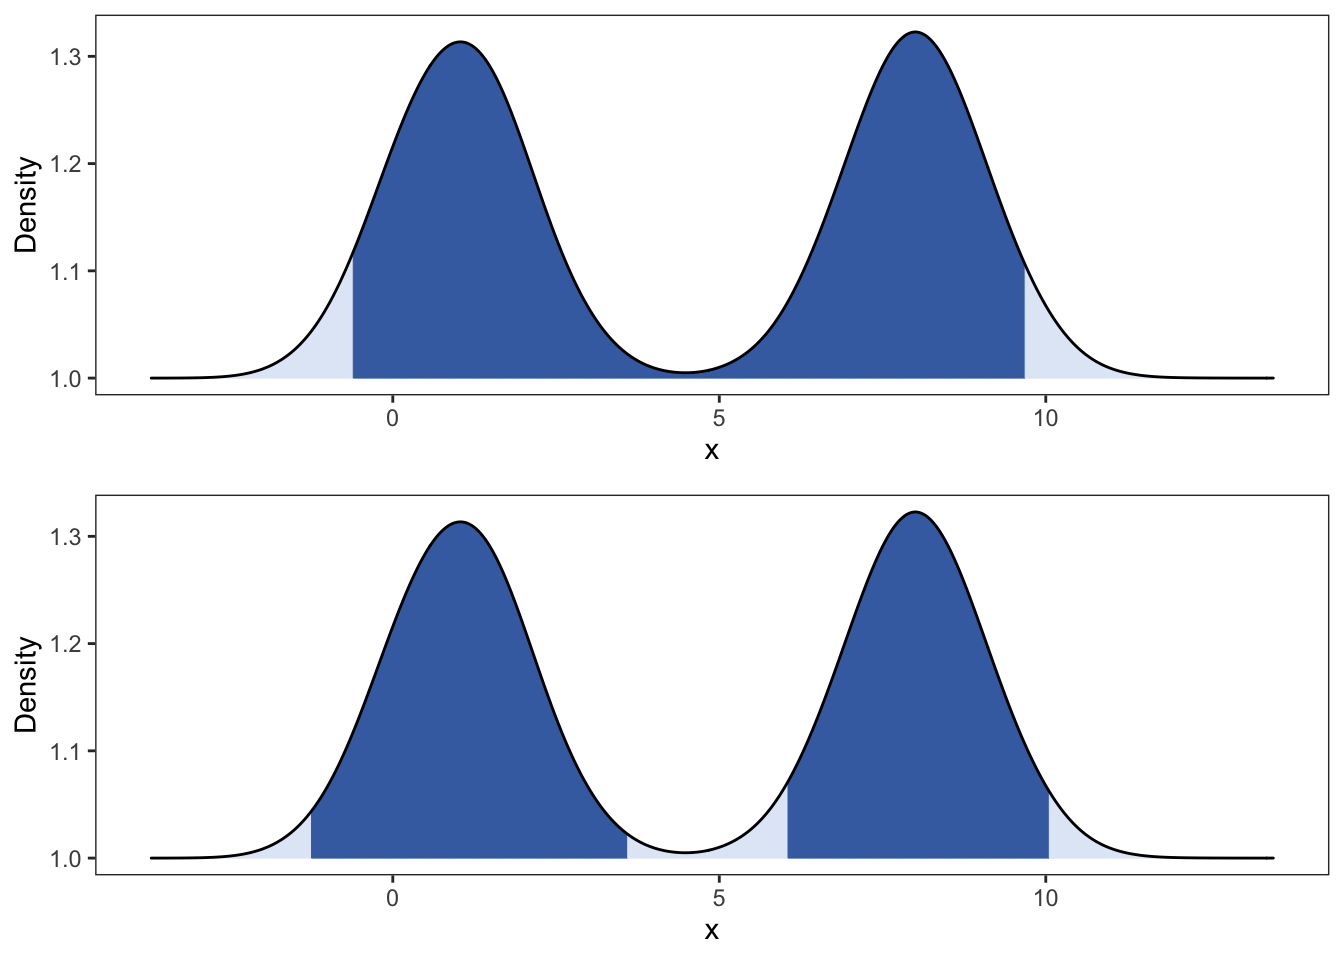
\includegraphics{1001-chapter01_files/figure-latex/unnamed-chunk-11-1} \end{center}

\begin{Shaded}
\begin{Highlighting}[]
\CommentTok{\# plot(cars) \# 效果同上}
\end{Highlighting}
\end{Shaded}

\textbf{结论:}随着汽车行驶速度的增加,刹车距离也在不断增加。

\hypertarget{ux6563ux70b9ux77e9ux9635ux56fe}{%
\subsubsection{散点矩阵图}\label{ux6563ux70b9ux77e9ux9635ux56fe}}

\textbf{概念介绍}:散点矩阵图将多个散点图组合起来,以便可以同时浏览多个二元变量关系,一定程度上克服了在平面上展示高维数据分布情况的困难。可以使用\texttt{plot()}或者\texttt{pairs()}进行绘制。

\textbf{适用}:高维数据

\begin{itemize}
\tightlist
\item
  \textbf{plot}
\end{itemize}

\begin{Shaded}
\begin{Highlighting}[]
\FunctionTok{plot}\NormalTok{(iris[, }\DecValTok{1}\SpecialCharTok{:}\DecValTok{4}\NormalTok{])}
\end{Highlighting}
\end{Shaded}

\begin{center}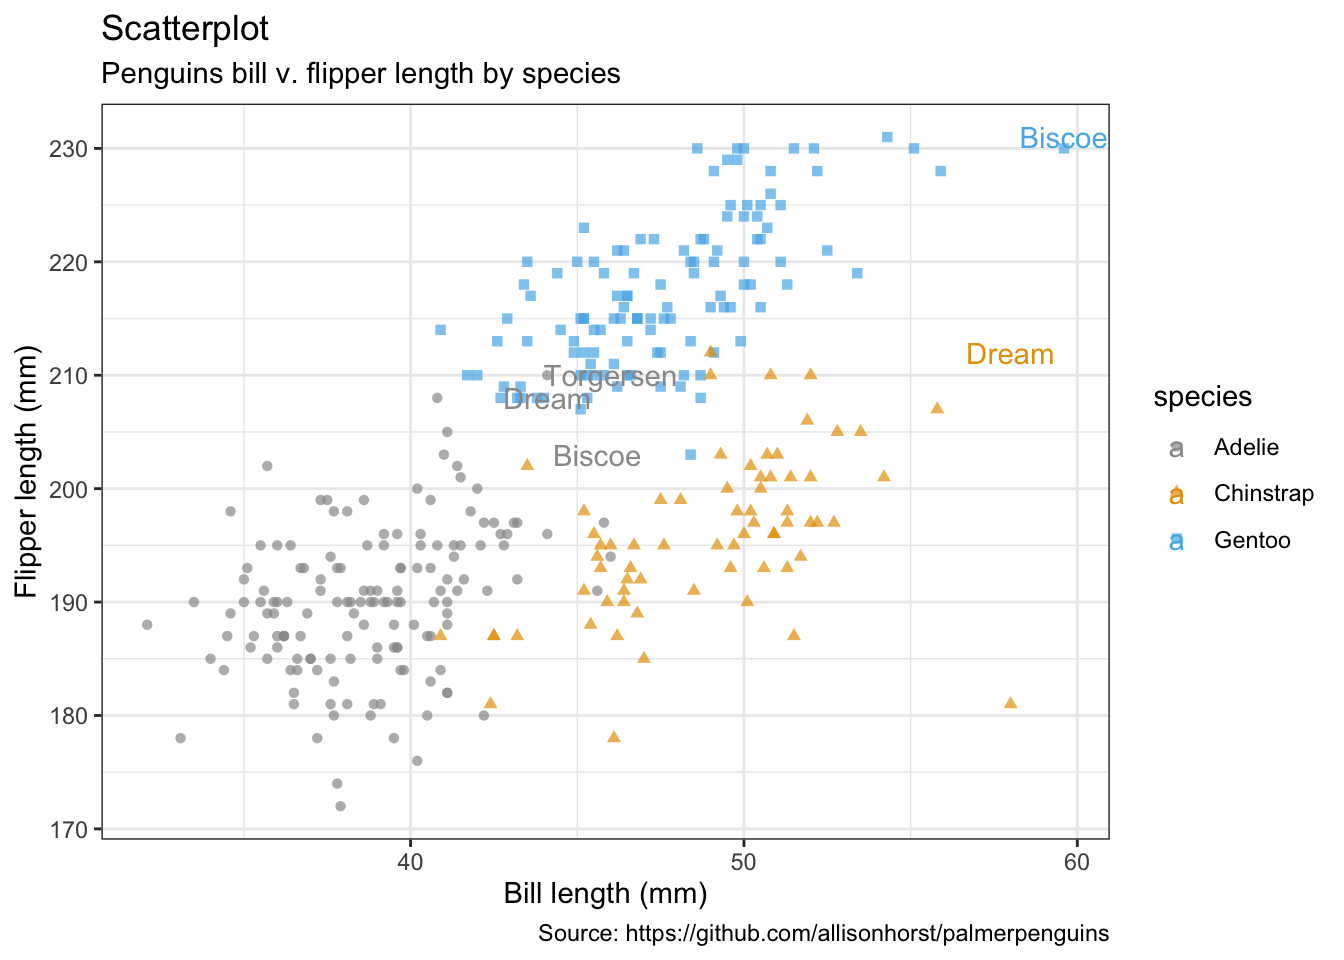
\includegraphics{1001-chapter01_files/figure-latex/unnamed-chunk-12-1} \end{center}

\textbf{结论:}花瓣长度(Petal.length)与花瓣宽度(Petal.Width)有明显的线性关系,其余属性之间的关系不是很明显。

\begin{itemize}
\tightlist
\item
  \textbf{pairs}
\end{itemize}

此外,R中还提供了另一个绘制散点矩阵图的函数------pairs函数,绘图对象有\textbf{数据框}和\textbf{公式}两种:

\begin{Shaded}
\begin{Highlighting}[]
\FunctionTok{pairs}\NormalTok{(iris[, }\DecValTok{1}\SpecialCharTok{:}\DecValTok{4}\NormalTok{])}
\FunctionTok{pairs}\NormalTok{(}\SpecialCharTok{\textasciitilde{}}\NormalTok{Sepal.Length }\SpecialCharTok{+}\NormalTok{ Sepal.Width }\SpecialCharTok{+}\NormalTok{ Petal.Length }\SpecialCharTok{+}\NormalTok{ Petal.Width, }\AttributeTok{data =}\NormalTok{ iris)  }\CommentTok{\# 效果同上}
\end{Highlighting}
\end{Shaded}

\begin{center}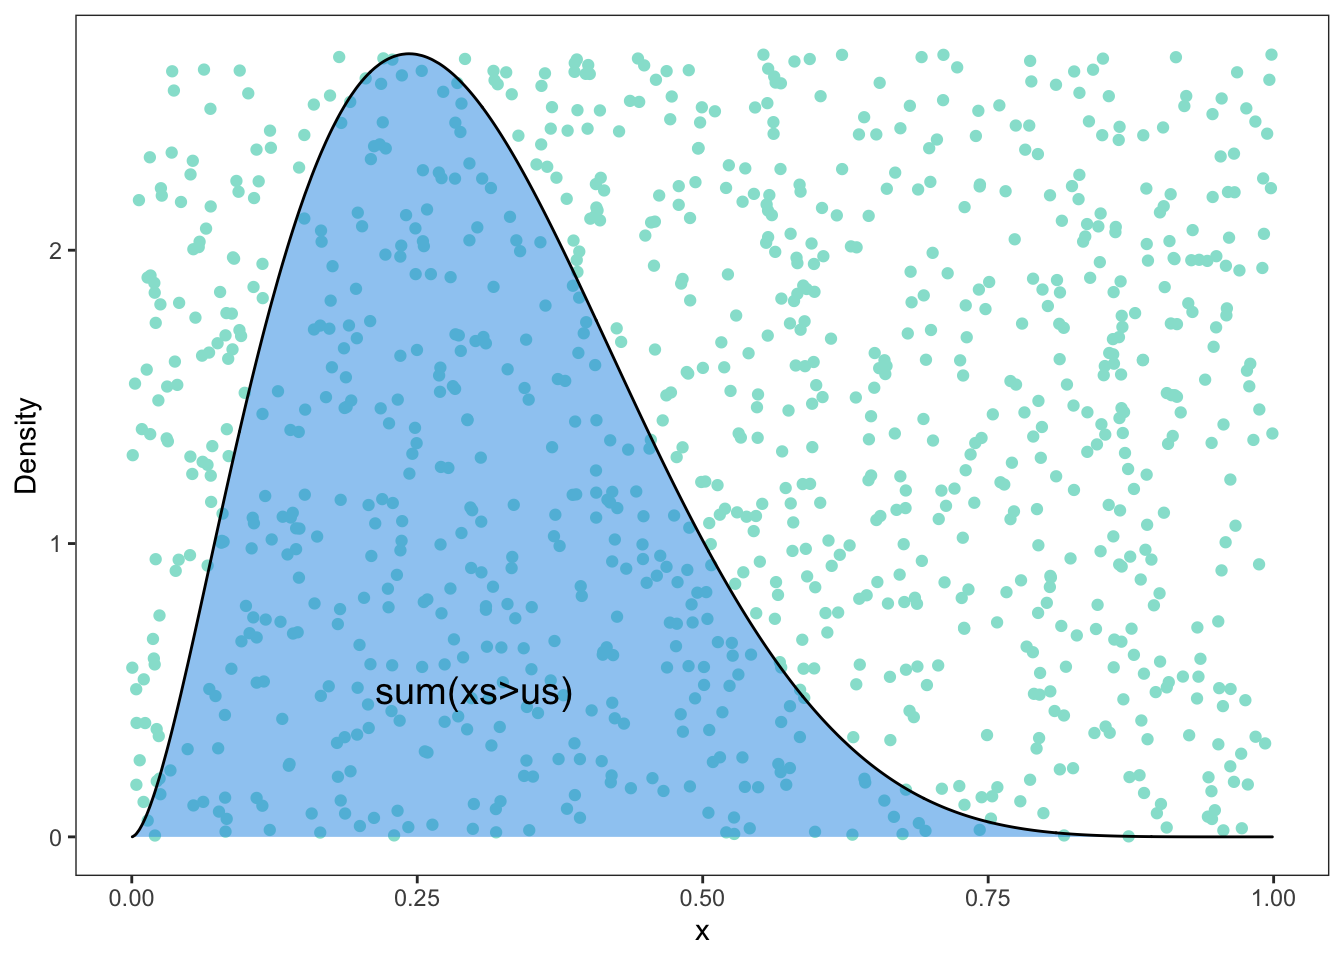
\includegraphics{1001-chapter01_files/figure-latex/unnamed-chunk-13-1} \end{center}

\hypertarget{ux591aux53d8ux91cfux76f8ux5173ux77e9ux9635ux56fe}{%
\subsubsection{多变量相关矩阵图}\label{ux591aux53d8ux91cfux76f8ux5173ux77e9ux9635ux56fe}}

\textbf{概念介绍}:多变量相关矩阵图是\textbf{相关系数矩阵}(correlation matrix)的可视化结果,显示了两两变量间的相关关系,对数据维度相对较大的数据有较好的展示效果。在R的\texttt{corrgram}包中的\texttt{corrgram}函数可绘制多变量相关矩阵图。

\textbf{数据介绍}:Mtcar数据集是1974年Motor Trend US杂志公布的32辆车的11个数据,包括燃料消耗和10个关于汽车设计与性能的数据。

\textbf{例子}:下面、根据这个数据集,绘制适用中不同元素描述相关性大小的图。

\begin{Shaded}
\begin{Highlighting}[]
\FunctionTok{library}\NormalTok{(corrgram)}
\FunctionTok{corrgram}\NormalTok{(mtcars)}
\end{Highlighting}
\end{Shaded}

\begin{center}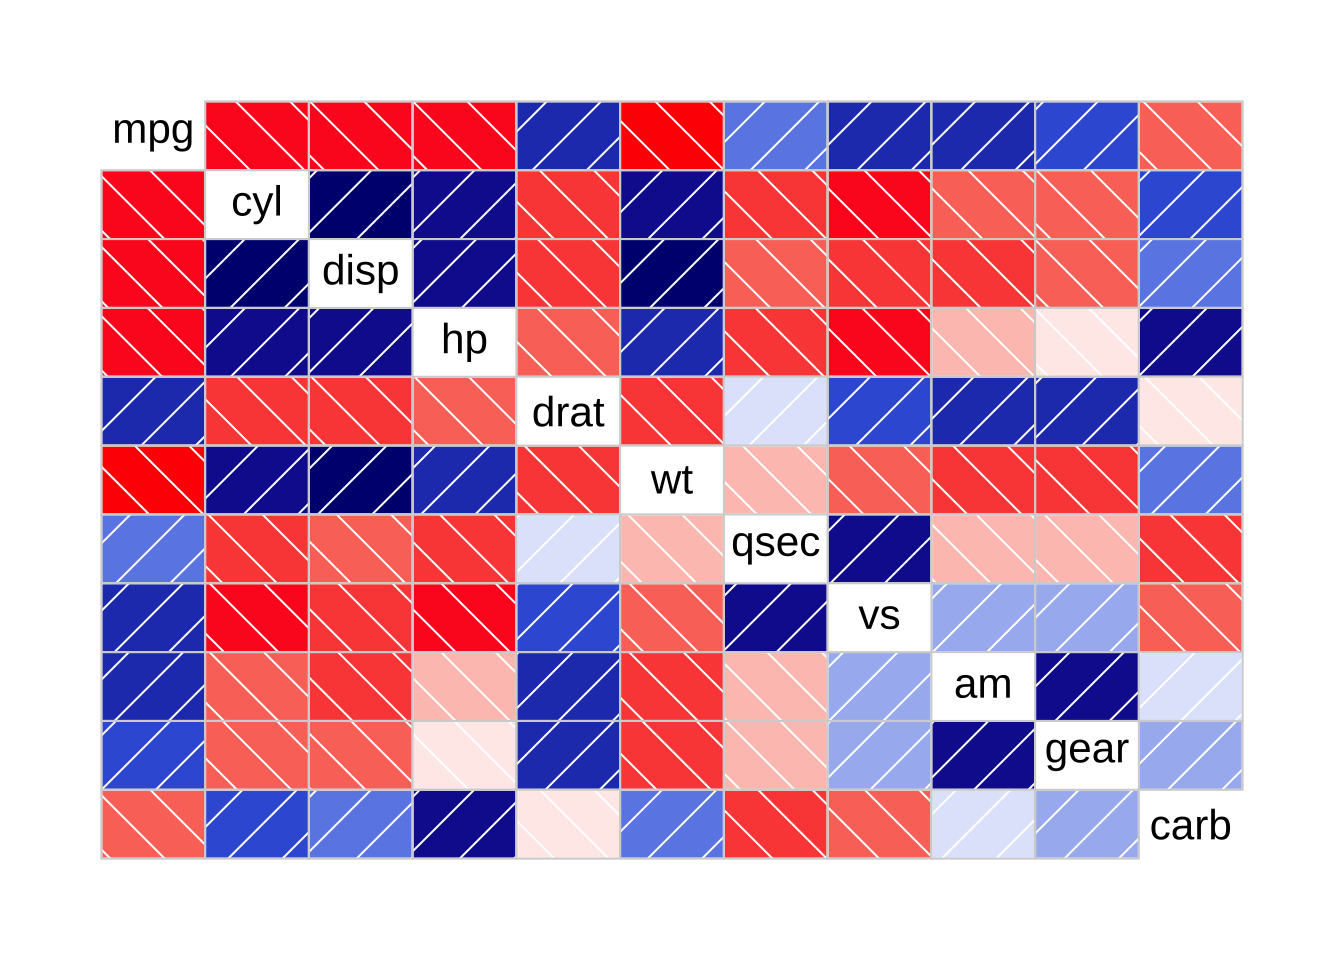
\includegraphics{1001-chapter01_files/figure-latex/unnamed-chunk-14-1} \end{center}

\begin{Shaded}
\begin{Highlighting}[]
\FunctionTok{corrgram}\NormalTok{(mtcars, }\AttributeTok{order =} \ConstantTok{TRUE}\NormalTok{, }\AttributeTok{upper.panel =}\NormalTok{ panel.ellipse, }\AttributeTok{main =} \StringTok{"Correlogram of mtcars intercorrelations"}\NormalTok{)}
\end{Highlighting}
\end{Shaded}

\begin{center}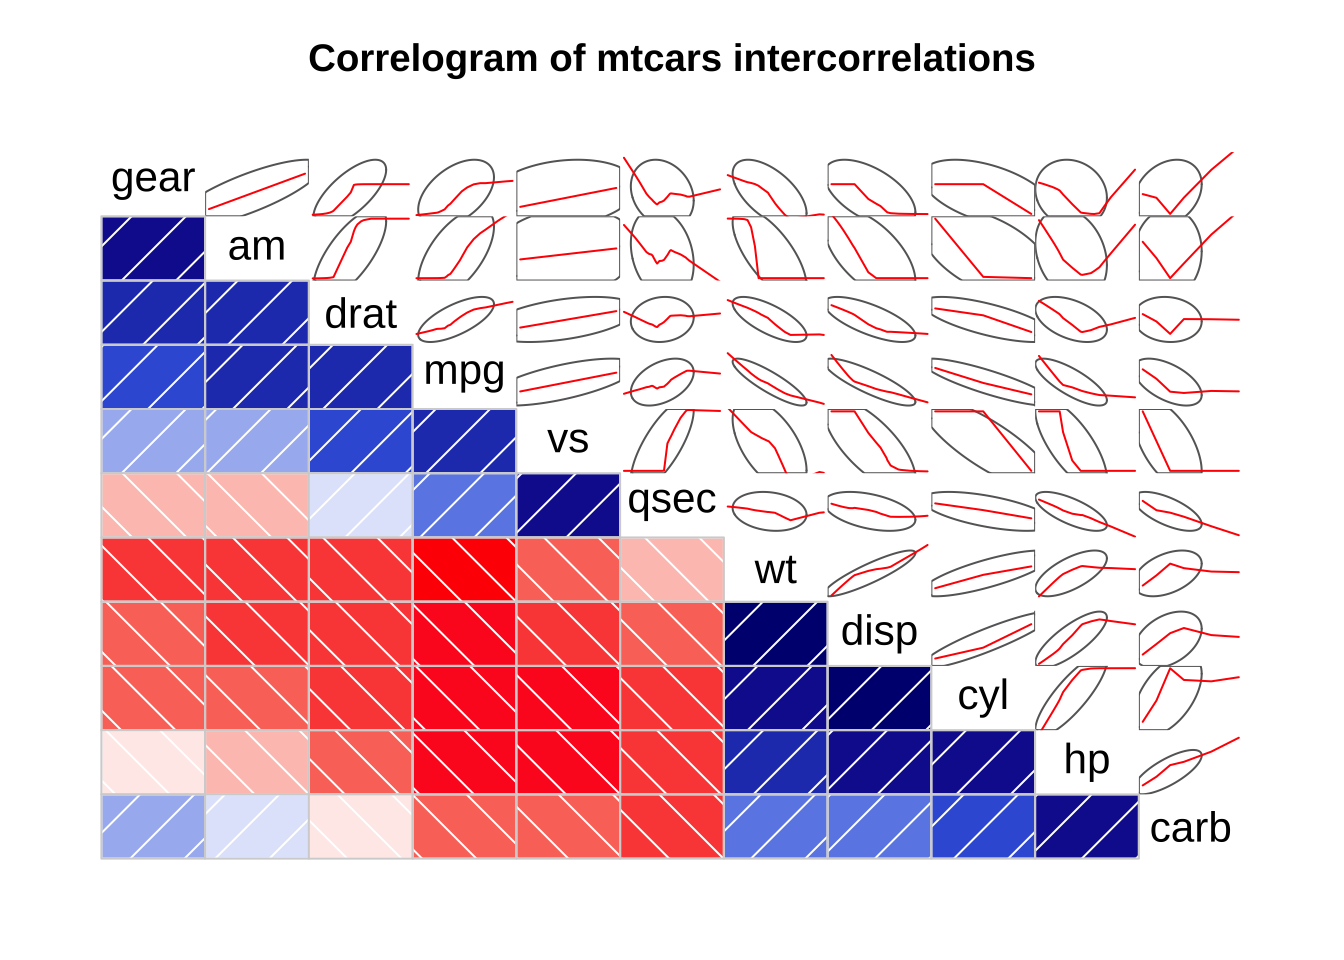
\includegraphics{1001-chapter01_files/figure-latex/unnamed-chunk-14-2} \end{center}

\begin{Shaded}
\begin{Highlighting}[]
\CommentTok{\# 相关图,主对角线上方绘制置信椭圆和平滑拟合曲线,主对角线下方绘制阴影}
\end{Highlighting}
\end{Shaded}

\textbf{结论}:\texttt{disp}与\texttt{cyl}呈正相关关系,且相关程度较高。此外,\texttt{mpg}与\texttt{wt}呈高度负相关,且\texttt{am}与\texttt{carb}基本没有关系。

这里可以对\texttt{upper.panel}和\texttt{lower.panel}进行设置,展示不同图形。具体可以通过帮助获得相信参数设置信息(\texttt{?corrgram})

\begin{Shaded}
\begin{Highlighting}[]
\CommentTok{\# 相关图,主对角线上方绘制散点图,主对角线下方绘制饼图}
\FunctionTok{corrgram}\NormalTok{(mtcars, }\AttributeTok{order =} \ConstantTok{TRUE}\NormalTok{, }\AttributeTok{upper.panel =}\NormalTok{ panel.pts, }\AttributeTok{lower.panel =}\NormalTok{ panel.pie, }
    \AttributeTok{main =} \StringTok{"Correlogram of mtcars intercorrelations"}\NormalTok{)}
\end{Highlighting}
\end{Shaded}

\begin{center}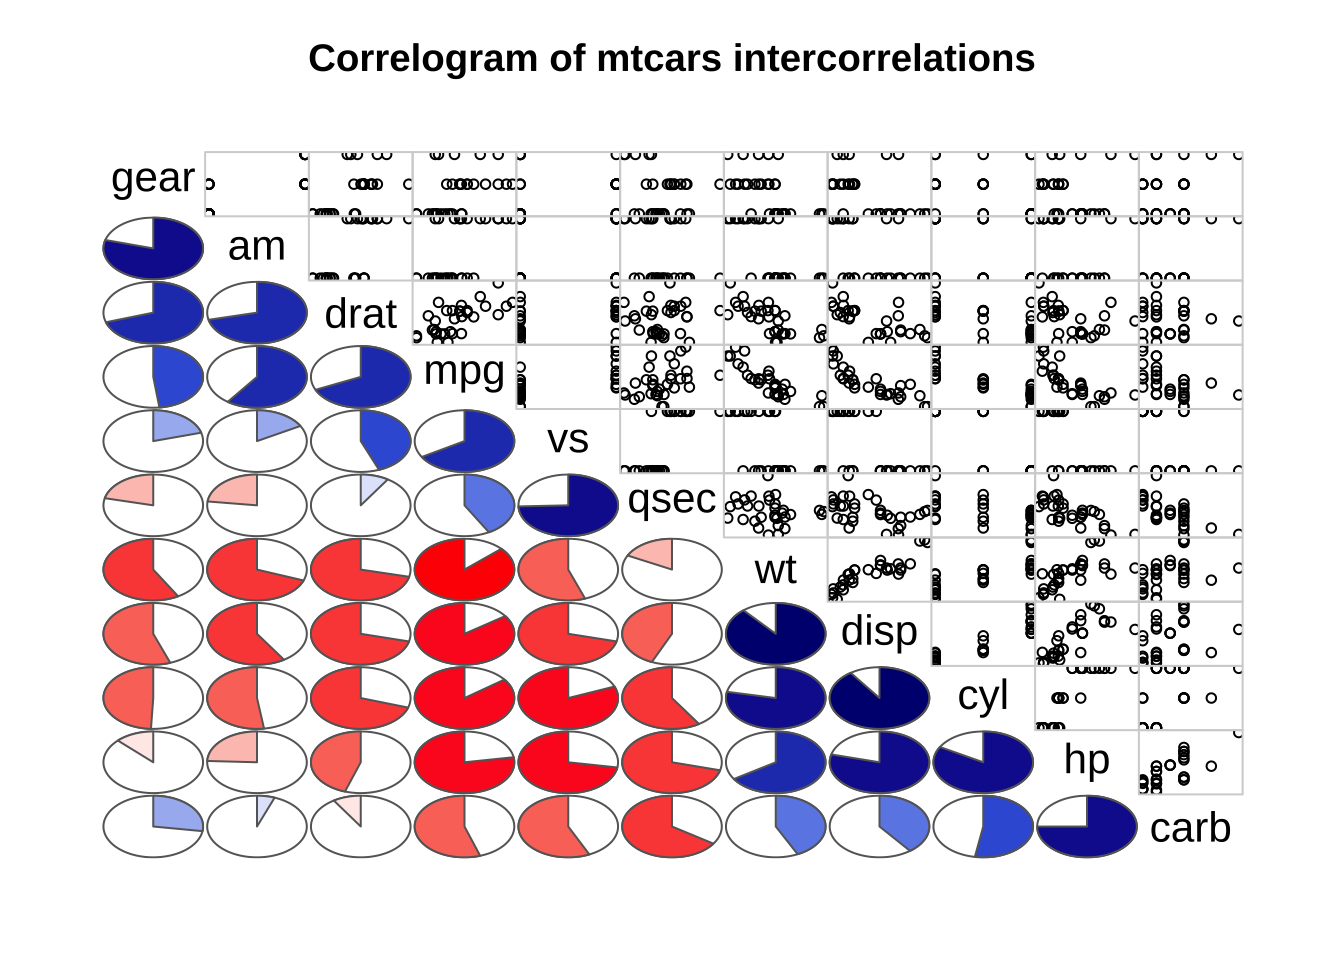
\includegraphics{1001-chapter01_files/figure-latex/unnamed-chunk-15-1} \end{center}

\begin{Shaded}
\begin{Highlighting}[]
\CommentTok{\# 相关图,主对角线上方绘制置信区间,主对角线下方绘制相关系数}
\FunctionTok{corrgram}\NormalTok{(mtcars, }\AttributeTok{order =} \ConstantTok{TRUE}\NormalTok{, }\AttributeTok{upper.panel =}\NormalTok{ panel.conf, }\AttributeTok{lower.panel =}\NormalTok{ panel.cor, }
    \AttributeTok{main =} \StringTok{"Correlogram of mtcars intercorrelations"}\NormalTok{)}
\end{Highlighting}
\end{Shaded}

\begin{center}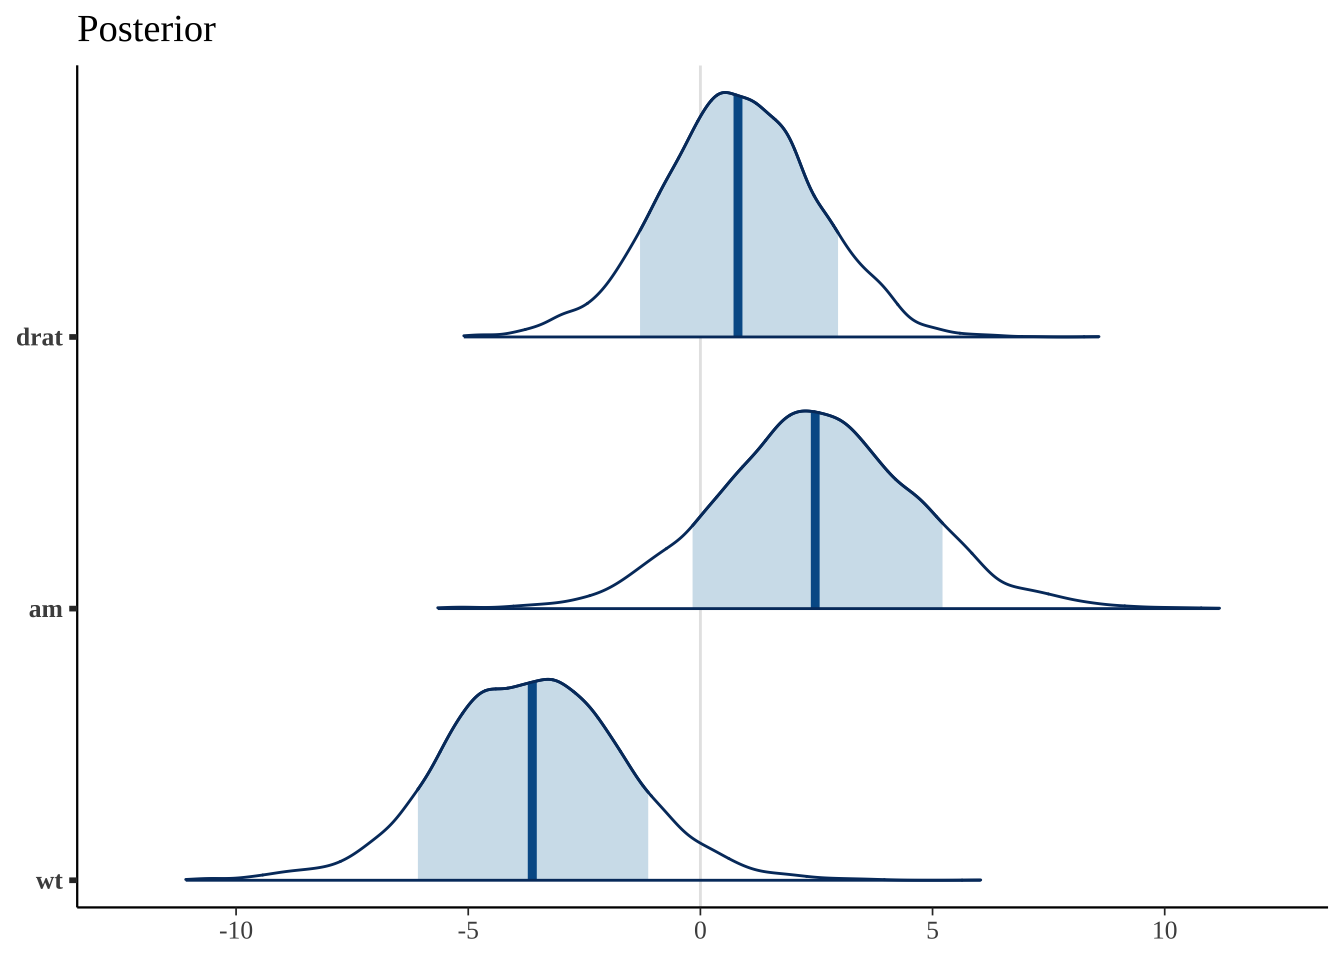
\includegraphics{1001-chapter01_files/figure-latex/unnamed-chunk-16-1} \end{center}

\hypertarget{ux7ed8ux5236ux5176ux4ed6ux56feux5f62}{%
\subsection{绘制其他图形}\label{ux7ed8ux5236ux5176ux4ed6ux56feux5f62}}

\hypertarget{ux6838ux5bc6ux5ea6ux56fe}{%
\subsubsection{核密度图}\label{ux6838ux5bc6ux5ea6ux56fe}}

\textbf{概念介绍}:sm包中\texttt{sm.density.compare}函数用于绘制核密度图,核密度图如果想用一条密度曲线而不是通过柱状来展示连续型变量的分布。

\textbf{特点}:相比直方图,密度图的一个优势是可以堆放,可用于比较组间差异。\texttt{sm.density.compare}函数可以直接堆放多条密度曲线。使用格式如下。

\texttt{sm.density.compare(x\ ,group,….)}

其中x是数值向量,group是分组向量,是因子型数据。

\begin{Shaded}
\begin{Highlighting}[]
\FunctionTok{library}\NormalTok{(sm)  }\CommentTok{\# 加载sm包}
\FunctionTok{sm.density.compare}\NormalTok{(mtcars}\SpecialCharTok{$}\NormalTok{wt, }\FunctionTok{factor}\NormalTok{(mtcars}\SpecialCharTok{$}\NormalTok{cyl))  }\CommentTok{\# 绘制核密度图}
\end{Highlighting}
\end{Shaded}

\begin{center}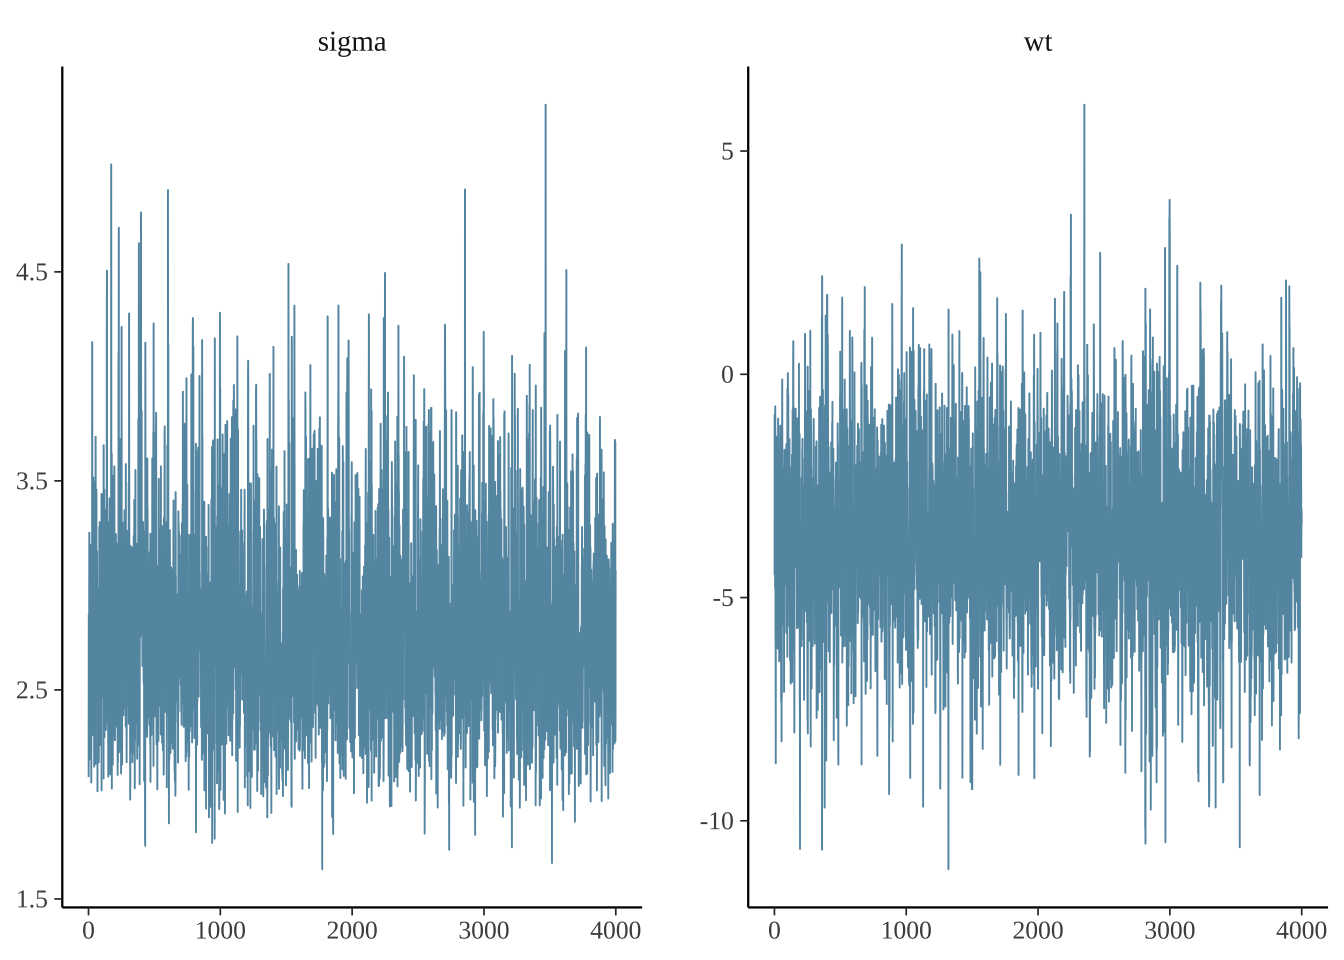
\includegraphics{1001-chapter01_files/figure-latex/unnamed-chunk-17-1} \end{center}

\hypertarget{ux5c0fux63d0ux7434ux56fe}{%
\subsubsection{小提琴图}\label{ux5c0fux63d0ux7434ux56fe}}

\textbf{概念介绍}:vioplot包中的vioplot函数用于绘制小提琴图,小提琴图是核密度图与箱线图的结合,本质是利用密度值生成的多边形,但该多边形同时还沿着一条直线作了另一半对称的``镜像'',这样两个左右或上下对称的多边形拼起来就形成了小提琴图的主体部分,最后一个箱线图也会被添加在小提琴的中轴线上。

使用格式如下。

\texttt{vioplot(\ x\ ,\ ...,\ \ range=1.5,\ \ h,\ \ ylim,\ names,\ \ horizontal=FALSE\ ,\ …)}

其中,x为数据源,可以是向量;range默认等于1.5;col是为每幅小提琴图指定颜色的向量。

\begin{Shaded}
\begin{Highlighting}[]
\FunctionTok{library}\NormalTok{(vioplot)  }\CommentTok{\# 加载vioplot包}
\FunctionTok{attach}\NormalTok{(mtcars)}
\FunctionTok{vioplot}\NormalTok{(wt[cyl }\SpecialCharTok{==} \DecValTok{4}\NormalTok{], wt[cyl }\SpecialCharTok{==} \DecValTok{6}\NormalTok{], wt[cyl }\SpecialCharTok{==} \DecValTok{8}\NormalTok{], }\AttributeTok{border =} \StringTok{"black"}\NormalTok{, }\AttributeTok{col =} \StringTok{"gray60"}\NormalTok{, }
    \AttributeTok{rectCol =} \StringTok{"blue"}\NormalTok{, }\AttributeTok{horizontal =} \ConstantTok{TRUE}\NormalTok{, }\AttributeTok{main =} \StringTok{"小提琴图"}\NormalTok{)  }\CommentTok{\# 绘制小提琴图}
\end{Highlighting}
\end{Shaded}

\begin{center}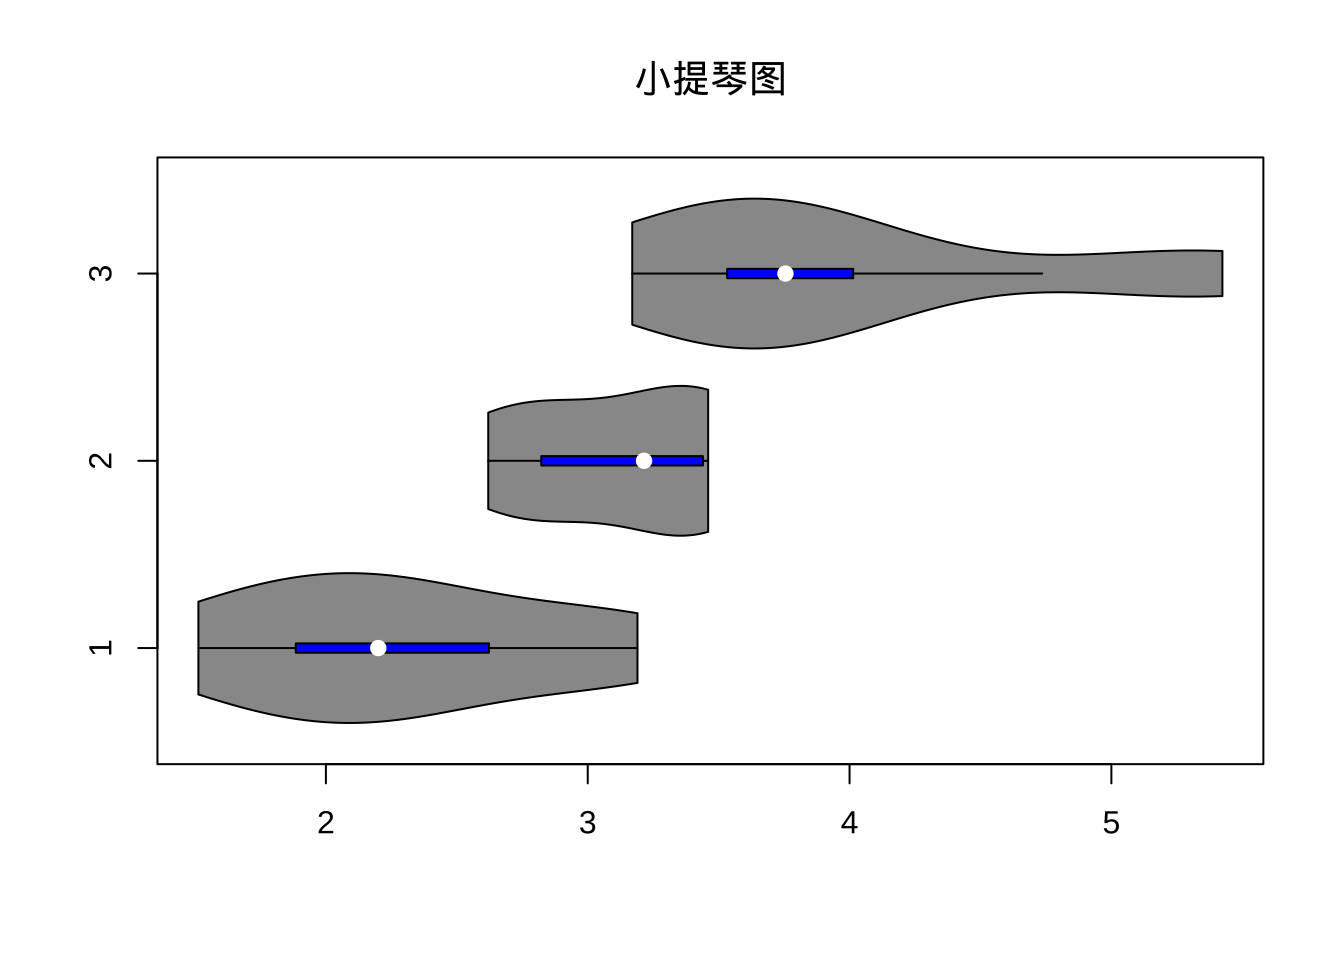
\includegraphics{1001-chapter01_files/figure-latex/unnamed-chunk-18-1} \end{center}

\begin{Shaded}
\begin{Highlighting}[]
\FunctionTok{boxplot}\NormalTok{(wt }\SpecialCharTok{\textasciitilde{}}\NormalTok{ cyl, }\AttributeTok{main =} \StringTok{"箱线图"}\NormalTok{, }\AttributeTok{horizontal =} \ConstantTok{TRUE}\NormalTok{, }\AttributeTok{pars =} \FunctionTok{list}\NormalTok{(}\AttributeTok{boxwex =} \FloatTok{0.1}\NormalTok{), }
    \AttributeTok{border =} \StringTok{"blue"}\NormalTok{)  }\CommentTok{\# 绘制箱线图}
\end{Highlighting}
\end{Shaded}

\begin{center}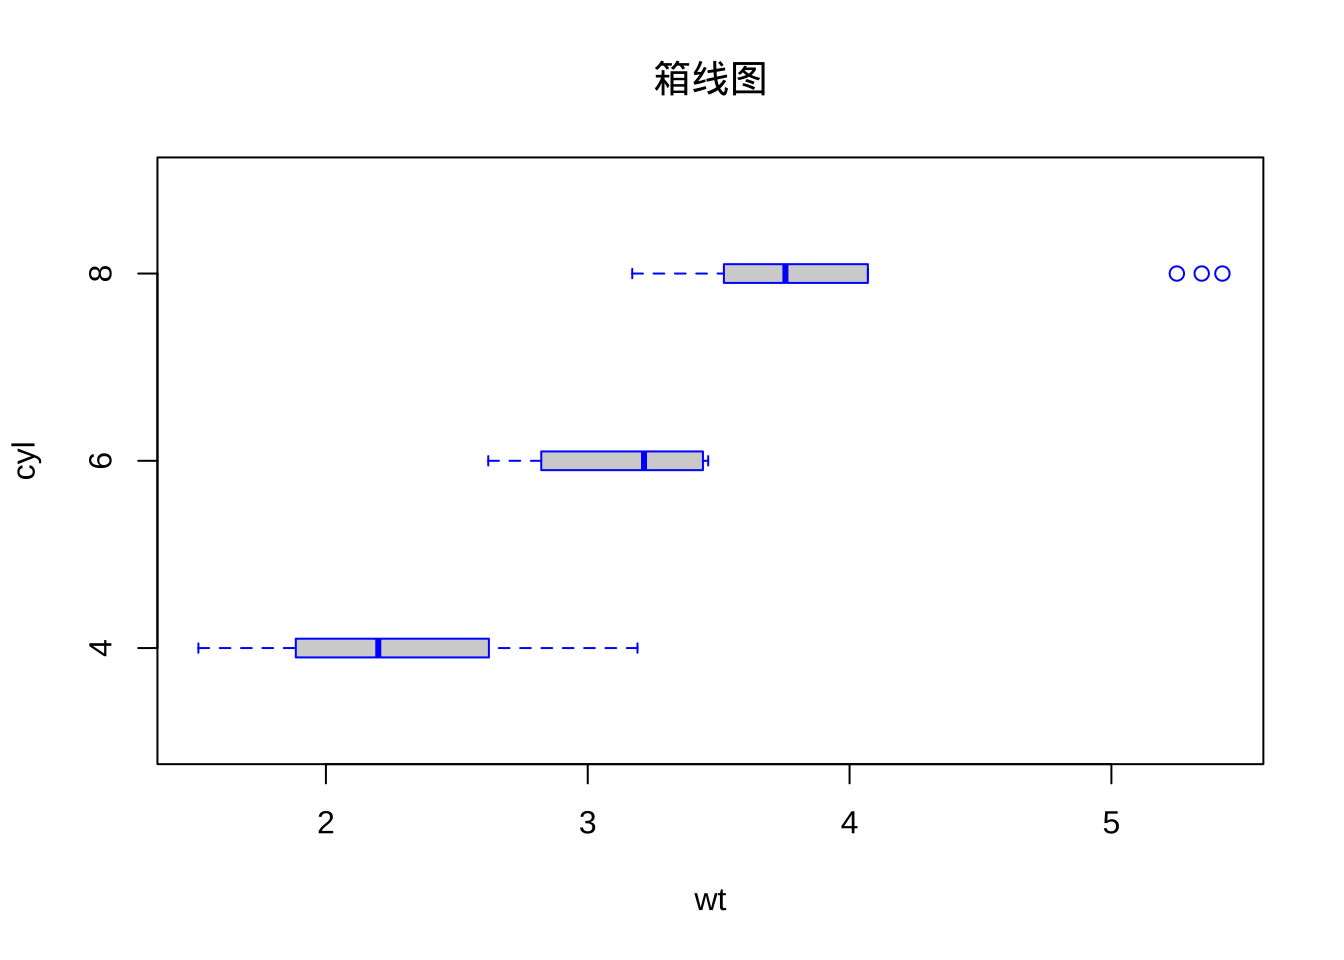
\includegraphics{1001-chapter01_files/figure-latex/unnamed-chunk-18-2} \end{center}

\hypertarget{qqux56fe}{%
\subsubsection{QQ图}\label{qqux56fe}}

\textbf{概念介绍}:查看经验分布和理论分布是否一致。将排序后的数据和理论分布的分位数进行比较后大致相等,说明了经验分布和理论分布相似。\texttt{qqplot()}函数用于绘制QQ图,QQ图检查数据是否服从某种分布。

使用格式如下:

\texttt{qqplot(x,\ y,,...);qqnorm(y,…)\ ;\ qqline(y)}

其中,x与y均为数据源,可以是向量。

\begin{Shaded}
\begin{Highlighting}[]
\FunctionTok{qqnorm}\NormalTok{(wt)  }\CommentTok{\#正态分布QQ图}
\FunctionTok{qqline}\NormalTok{(wt)  }\CommentTok{\#QQ线}
\end{Highlighting}
\end{Shaded}

\begin{center}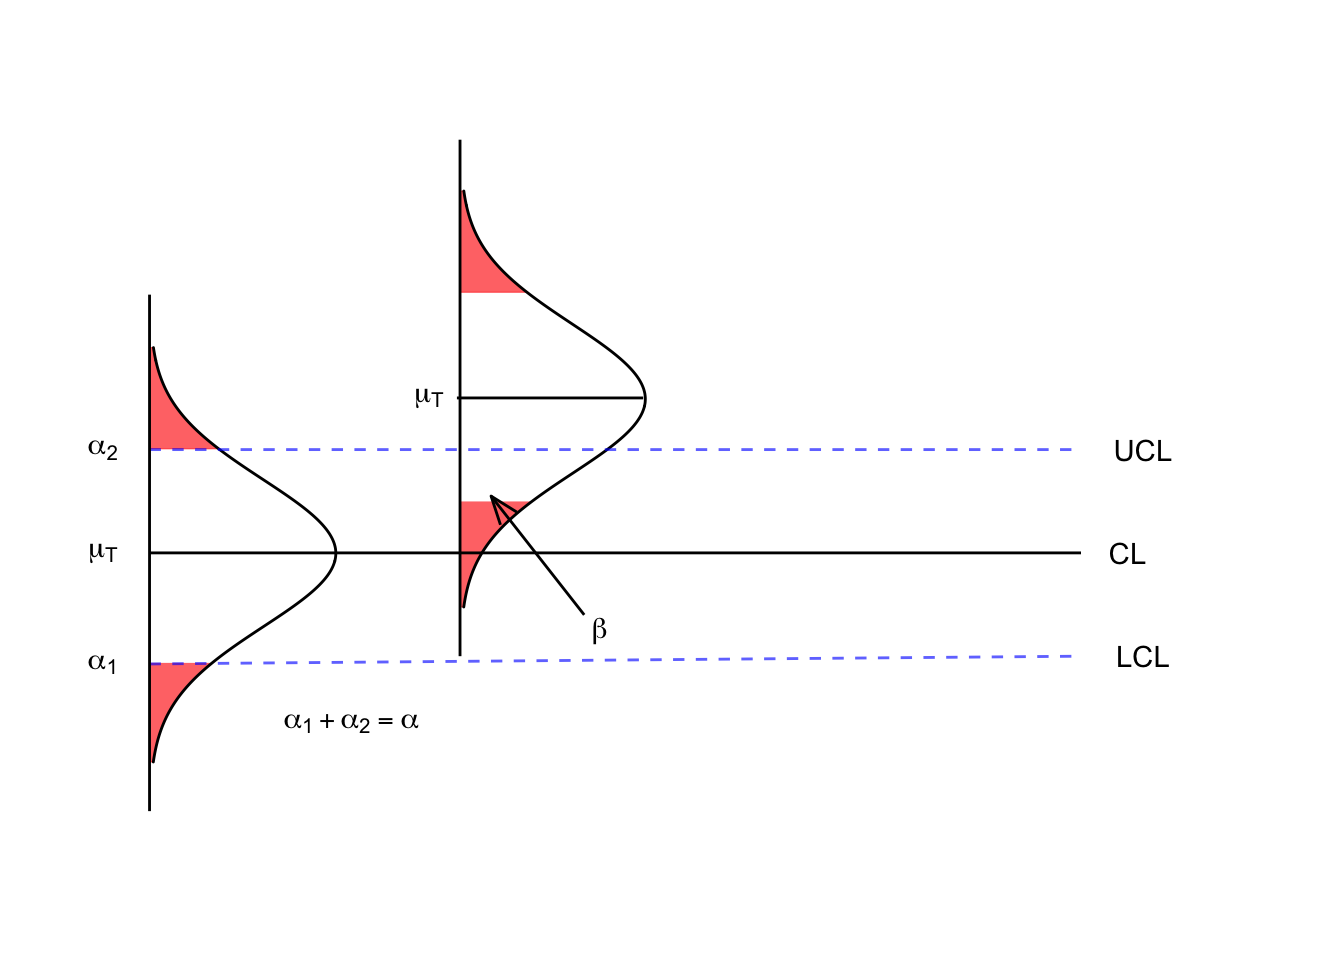
\includegraphics{1001-chapter01_files/figure-latex/unnamed-chunk-19-1} \end{center}

\hypertarget{ux7b49ux9ad8ux56fe}{%
\subsubsection{等高图}\label{ux7b49ux9ad8ux56fe}}

\textbf{概念介绍}:数据形式:两个数值向量x、y和一个相应的矩阵z。x、y交叉组合之后形成的是一个``网格'',z是这个网格上的高度数值,将平面上对应的z值(高度)相等的点连接起来形成的线就是等高线。对x、y进行核密度估计,得到一个密度值矩阵,然后用x、y以及这个密度值矩阵作等高图。由于密度值反映的是某个位置上数据的密集程度,等高图就展示了一个聚类现象。

使用格式如下

\texttt{contour(x=,y=,z,nlevels=,levels=,labels=\ ,method=,...)}

\begin{Shaded}
\begin{Highlighting}[]
\FunctionTok{library}\NormalTok{(KernSmooth)  }\CommentTok{\# 计算二维核密度的包}
\NormalTok{mtcars1 }\OtherTok{=} \FunctionTok{data.frame}\NormalTok{(wt, mpg)}
\NormalTok{est }\OtherTok{=} \FunctionTok{bkde2D}\NormalTok{(mtcars1, }\FunctionTok{apply}\NormalTok{(mtcars1, }\DecValTok{2}\NormalTok{, dpik))  }\CommentTok{\# 计算二维核密度}
\FunctionTok{contour}\NormalTok{(est}\SpecialCharTok{$}\NormalTok{x1, est}\SpecialCharTok{$}\NormalTok{x2, est}\SpecialCharTok{$}\NormalTok{fhat, }\AttributeTok{nlevels =} \DecValTok{15}\NormalTok{, }\AttributeTok{col =} \StringTok{"darkgreen"}\NormalTok{, }\AttributeTok{xlab =} \StringTok{"wt"}\NormalTok{, }\AttributeTok{ylab =} \StringTok{"mpg"}\NormalTok{)  }\CommentTok{\# 画等高图}
\FunctionTok{points}\NormalTok{(mtcars1)  }\CommentTok{\# 添加散点}
\end{Highlighting}
\end{Shaded}

\begin{center}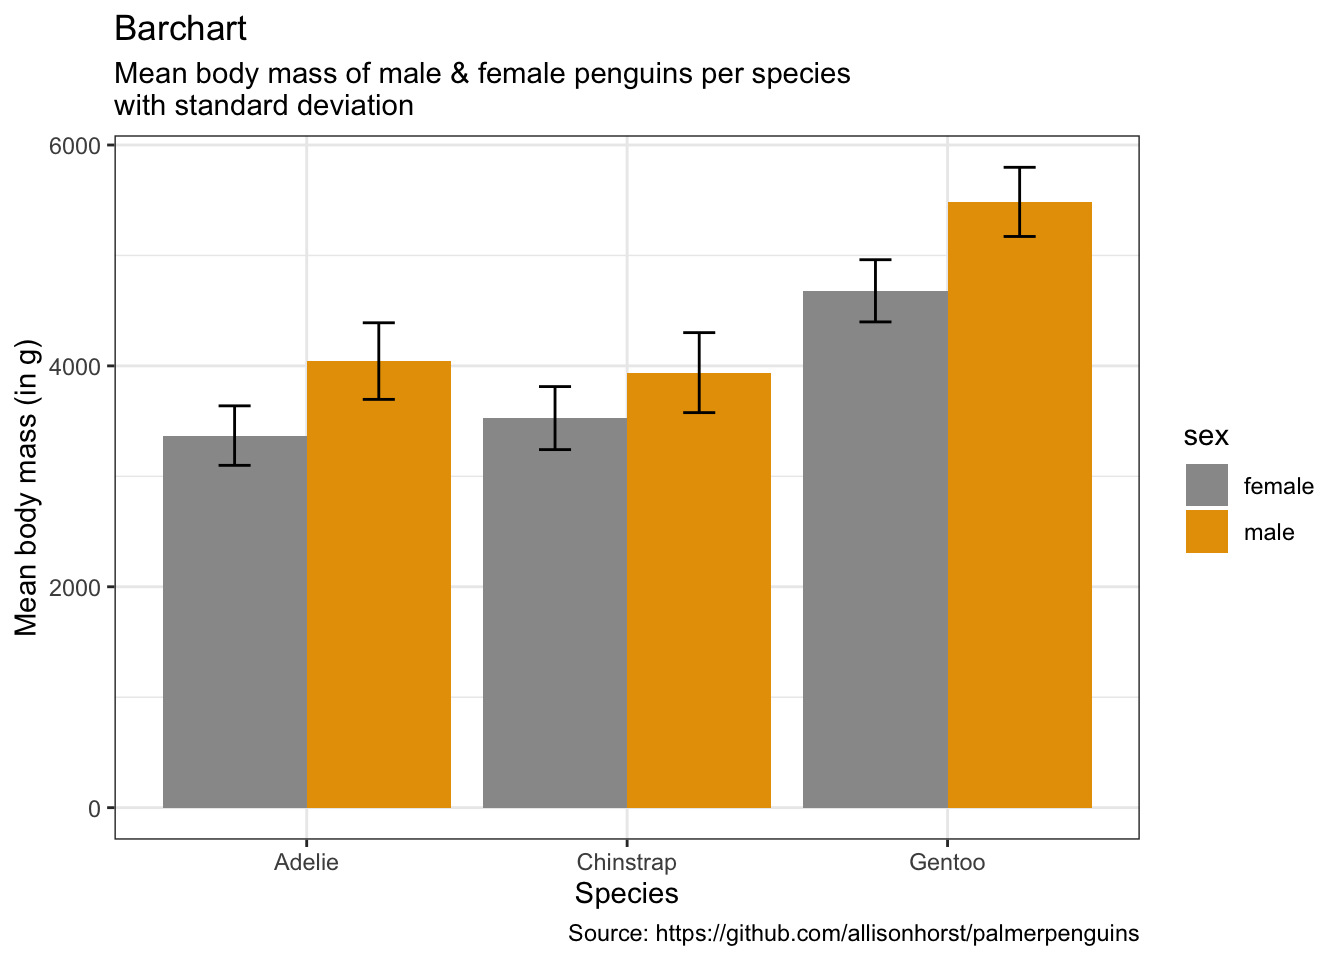
\includegraphics{1001-chapter01_files/figure-latex/unnamed-chunk-20-1} \end{center}

\hypertarget{ux4feeux6539ux56feux5f62ux53c2ux6570}{%
\section{修改图形参数}\label{ux4feeux6539ux56feux5f62ux53c2ux6570}}

R是一个功能强大的图形构建平台,可以通过逐条输入语句构建图形元素(\textbf{颜色、点、线、文本以及图例}等),逐渐完善图形特征,直至得到想要的效果。图形元素的显示可以用图形函数和绘图参数来改良,也可以用绘制图形元素的基础函数来控制。

\hypertarget{ux4feeux6539ux989cux8272}{%
\subsection{修改颜色}\label{ux4feeux6539ux989cux8272}}

R语言通过设置绘图参数col来改变\textbf{图像、坐标轴、文字、点、线}等的颜色。关于颜色的函数大致可以分为下面三类:

\hypertarget{ux56faux5b9aux989cux8272ux9009ux62e9ux51fdux6570}{%
\subsubsection{固定颜色选择函数}\label{ux56faux5b9aux989cux8272ux9009ux62e9ux51fdux6570}}

R语言提供了自带的固定种类的颜色,主要涉及的是colors函数,该函数可以生成657中颜色名称,代表657种颜色,可以通过以下代码查看R自带颜色的前20中颜色的名称。

\begin{Shaded}
\begin{Highlighting}[]
\FunctionTok{colors}\NormalTok{()[}\DecValTok{1}\SpecialCharTok{:}\DecValTok{20}\NormalTok{]}
\end{Highlighting}
\end{Shaded}

\begin{verbatim}
##  [1] "white"         "aliceblue"     "antiquewhite"  "antiquewhite1"
##  [5] "antiquewhite2" "antiquewhite3" "antiquewhite4" "aquamarine"   
##  [9] "aquamarine1"   "aquamarine2"   "aquamarine3"   "aquamarine4"  
## [13] "azure"         "azure1"        "azure2"        "azure3"       
## [17] "azure4"        "beige"         "bisque"        "bisque1"
\end{verbatim}

\begin{Shaded}
\begin{Highlighting}[]
\CommentTok{\# colors()}
\FunctionTok{plot}\NormalTok{(}\DecValTok{1}\SpecialCharTok{:}\DecValTok{10}\NormalTok{, }\AttributeTok{col =} \FunctionTok{cm.colors}\NormalTok{(}\DecValTok{1}\NormalTok{))}
\end{Highlighting}
\end{Shaded}

\begin{center}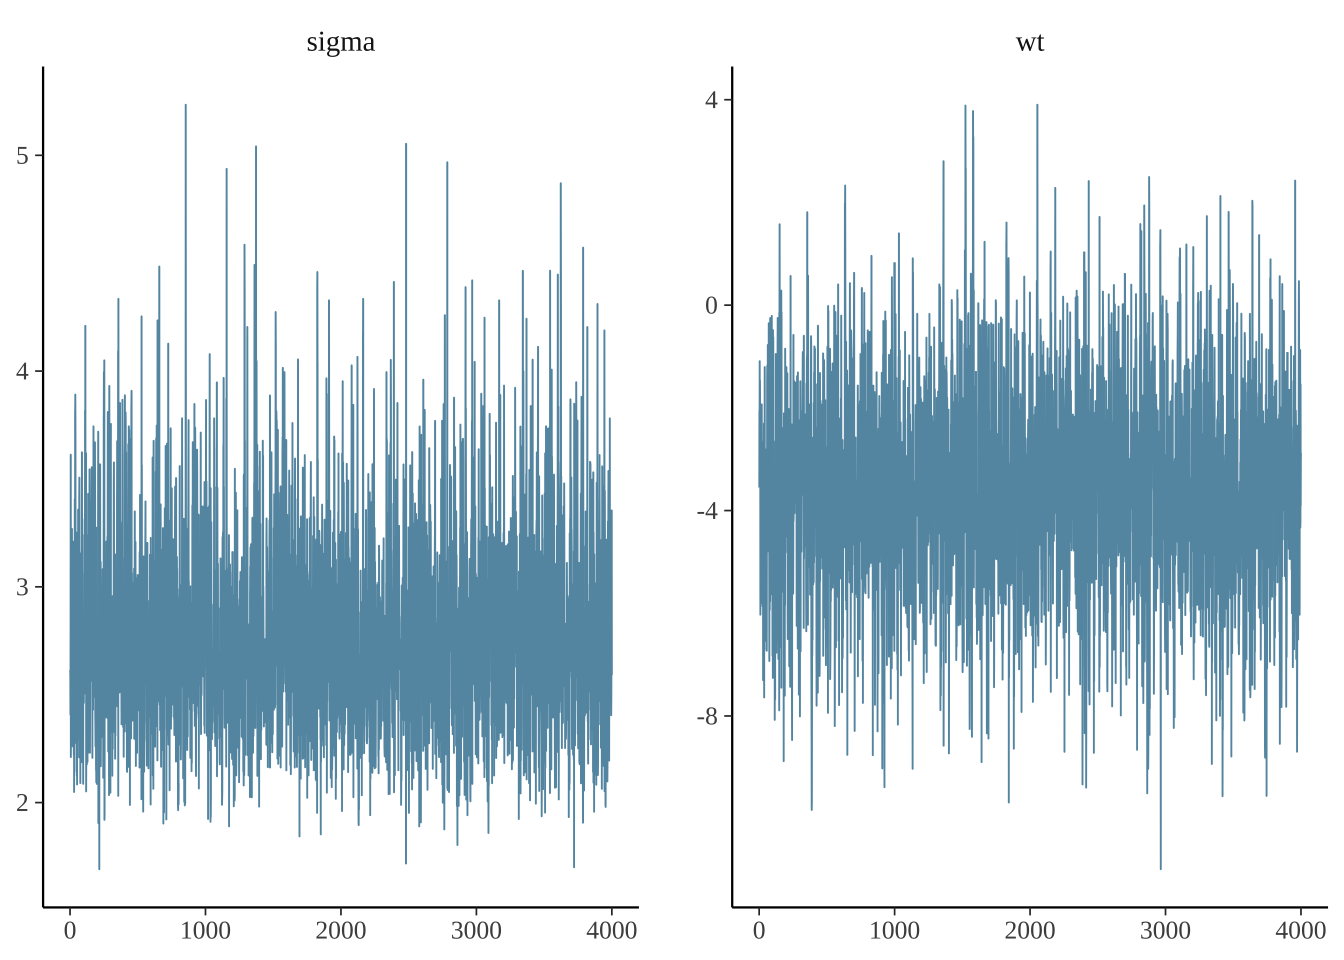
\includegraphics{1001-chapter01_files/figure-latex/unnamed-chunk-21-1} \end{center}

通过palette函数固定调色板,只要设定好了调色板,它的取值就不会再改变(直到下一次重新设定调色板)。

\begin{Shaded}
\begin{Highlighting}[]
\FunctionTok{palette}\NormalTok{()  }\CommentTok{\#返回当前的调色板设置,此时为默认值}
\DocumentationTok{\#\# [1] "black"   "\#DF536B" "\#61D04F" "\#2297E6" "\#28E2E5" "\#CD0BBC" "\#F5C710"}
\DocumentationTok{\#\# [8] "gray62"}
\FunctionTok{palette}\NormalTok{(}\FunctionTok{colors}\NormalTok{()[}\DecValTok{1}\SpecialCharTok{:}\DecValTok{10}\NormalTok{])  }\CommentTok{\#重新设置调色板为colors的前10种颜色}
\FunctionTok{palette}\NormalTok{()  }\CommentTok{\#返回当前的调色板设置,此时为colors()的前10种颜色}
\DocumentationTok{\#\#  [1] "white"         "aliceblue"     "antiquewhite"  "antiquewhite1"}
\DocumentationTok{\#\#  [5] "antiquewhite2" "antiquewhite3" "antiquewhite4" "aquamarine"   }
\DocumentationTok{\#\#  [9] "aquamarine"    "aquamarine2"}
\FunctionTok{palette}\NormalTok{(}\StringTok{"default"}\NormalTok{)  }\CommentTok{\#恢复默认的调色板设置}
\end{Highlighting}
\end{Shaded}

\textbf{例子}:

\begin{Shaded}
\begin{Highlighting}[]
\FunctionTok{plot}\NormalTok{(iris}\SpecialCharTok{$}\NormalTok{Sepal.Length, iris}\SpecialCharTok{$}\NormalTok{Sepal.Width, }\AttributeTok{col =}\NormalTok{ iris}\SpecialCharTok{$}\NormalTok{Species)}
\end{Highlighting}
\end{Shaded}

\begin{center}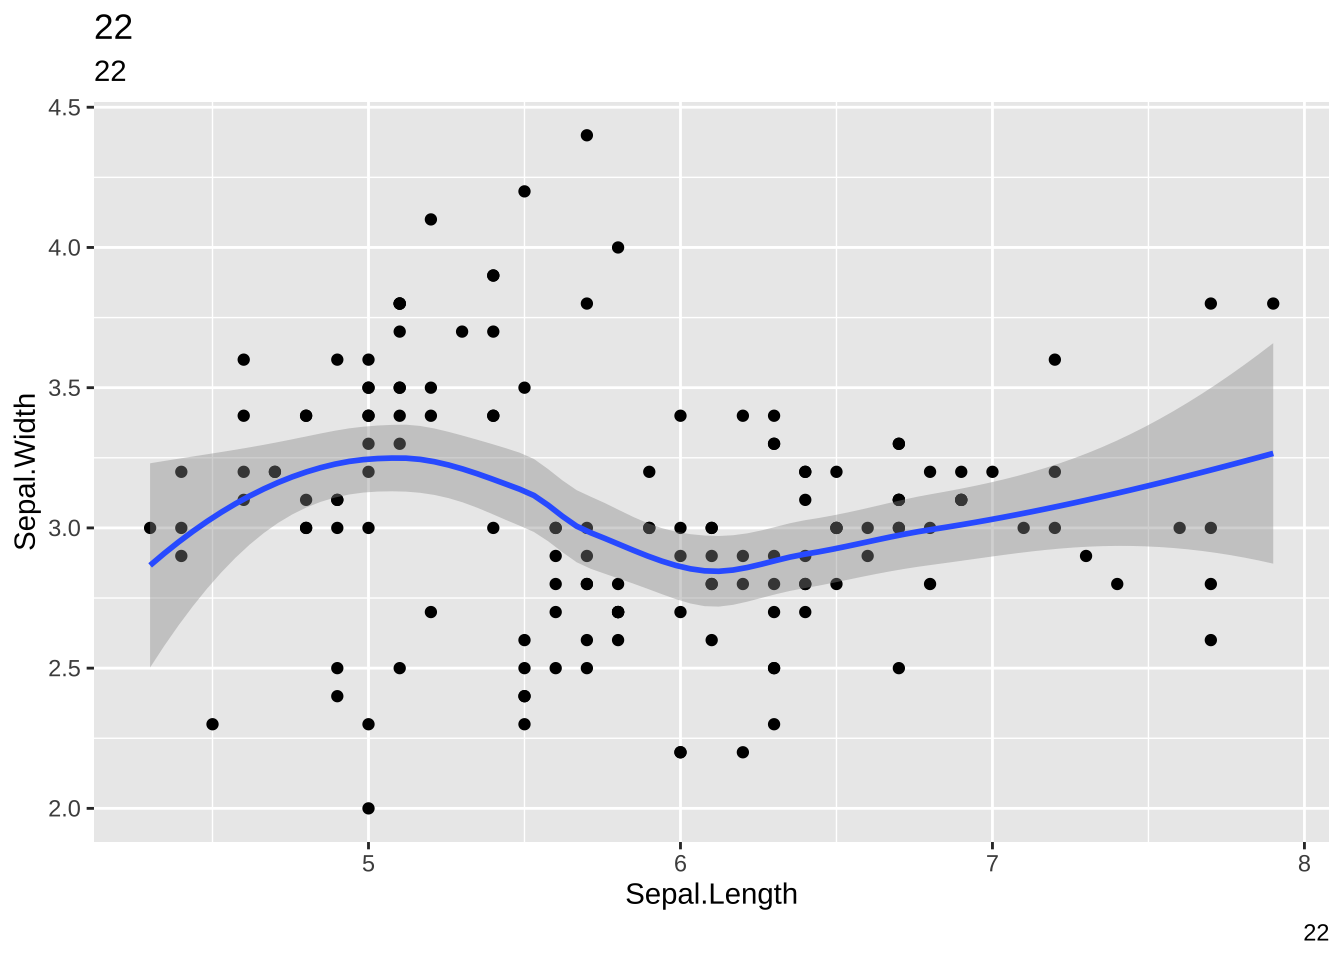
\includegraphics{1001-chapter01_files/figure-latex/unnamed-chunk-23-1} \end{center}

\begin{Shaded}
\begin{Highlighting}[]
\CommentTok{\# Species为因子型数据,setosa versicolor virginica分别对应数字1,2,3,}
\CommentTok{\# 即等价于col = rep(1:3, each = 50)}
\end{Highlighting}
\end{Shaded}

\hypertarget{ux6e10ux53d8ux8272ux751fux6210ux51fdux6570}{%
\subsubsection{渐变色生成函数}\label{ux6e10ux53d8ux8272ux751fux6210ux51fdux6570}}

除了固定颜色选择函数外,R还提供了一系列渐变颜色生成函数,这些函数用来控制颜色值\textbf{逐步变化}。

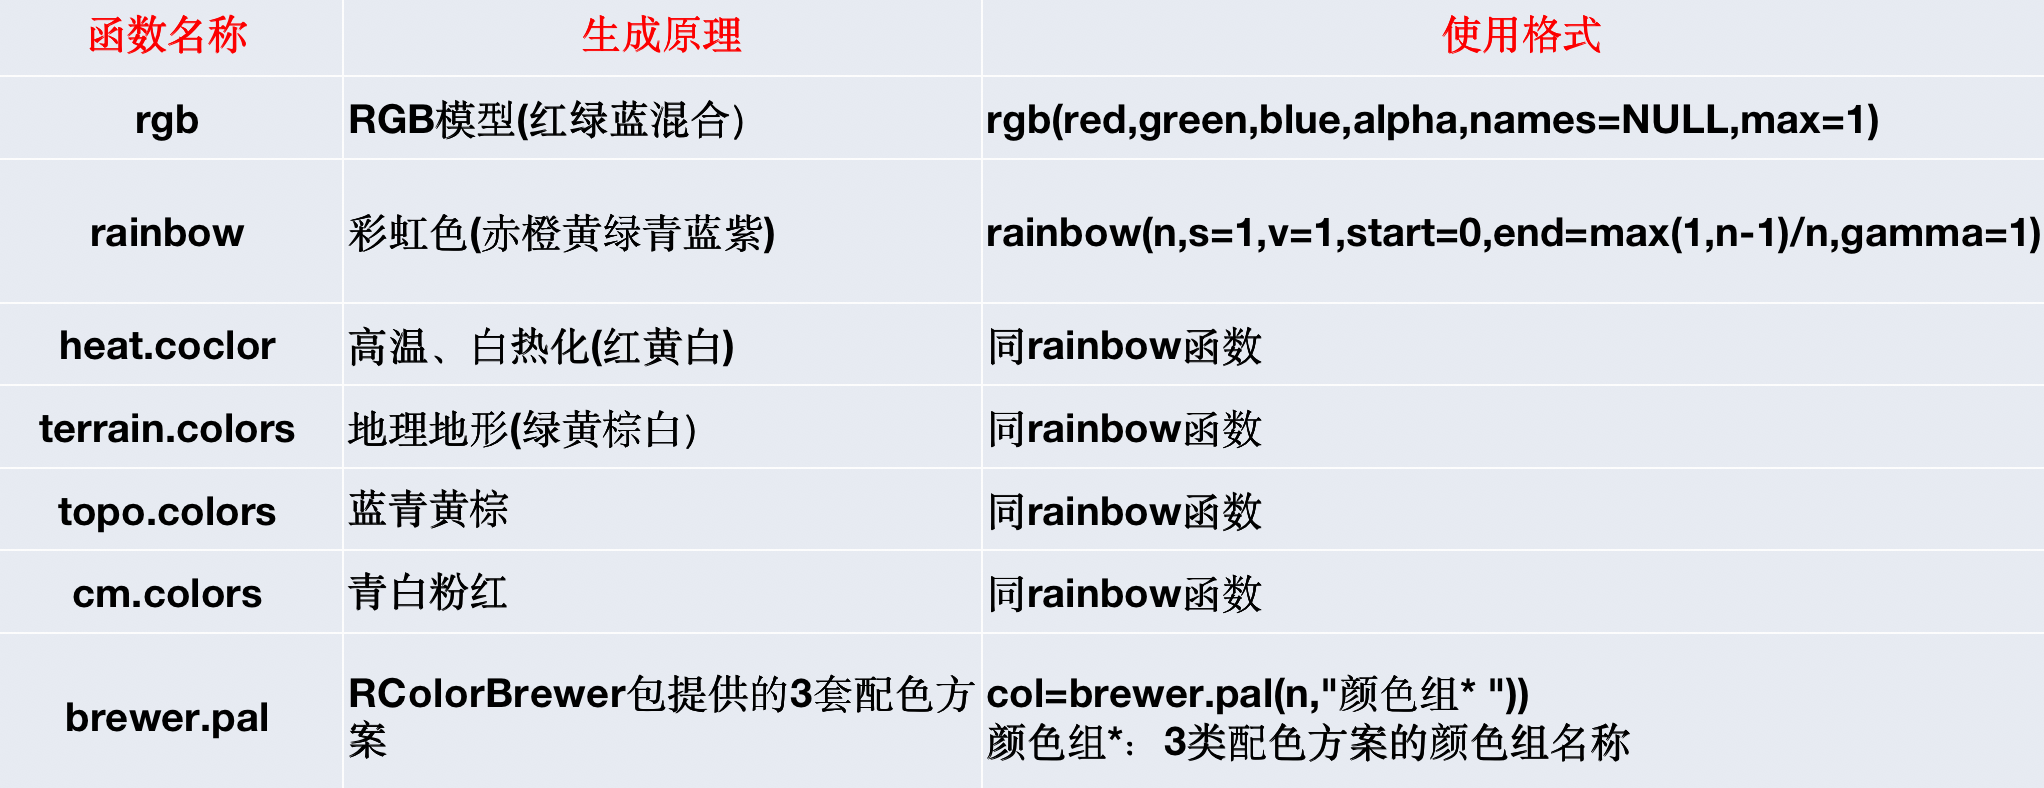
\includegraphics{figure/14.png}

rgb函数把RGB颜色转化为十六进制数值,使用格式前四个参数都取值于区间{[}0, max{]},names参数用来指定生成颜色向量的名称。red,green,blue参数的值越大就说明该颜色的成分越高。alpha指的是颜色的透明度,取0表示完全透明,取最大值表示完全不透明(默认完全不透明)。

\texttt{rainbow}函数、\texttt{heat.coclor}函数、\texttt{terrain.colors}函数、\texttt{topo.colors}函数、\texttt{cm.colors}函数是主题配色函数,使用格式中n设定产生颜色的数目,start和end设定彩虹颜色的一个子集,生成的颜色将从这个子集中选取。

\begin{center}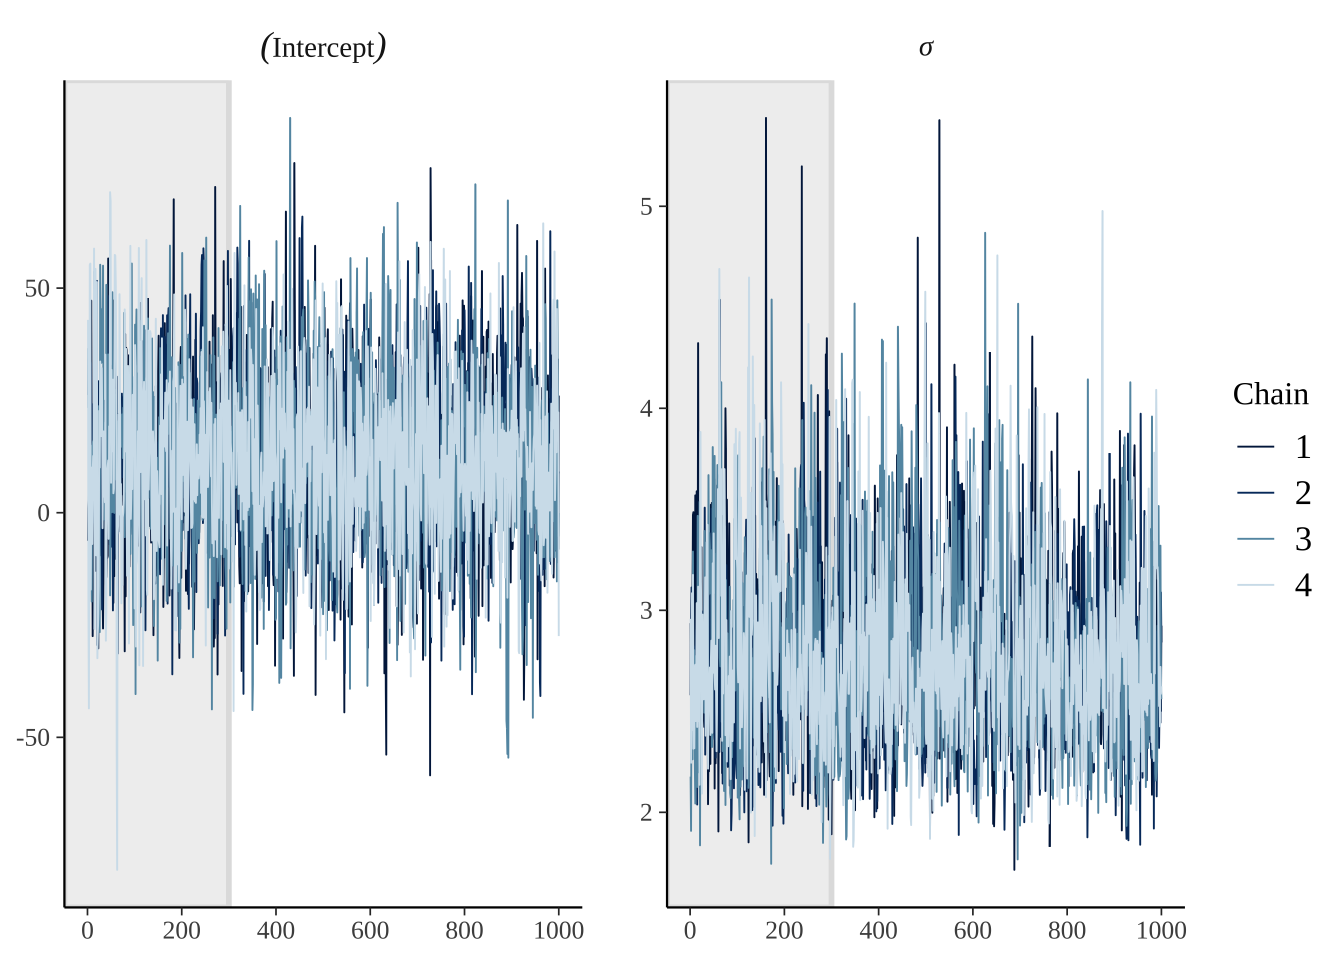
\includegraphics{1001-chapter01_files/figure-latex/unnamed-chunk-24-1} \end{center}

\hypertarget{rcolorbrewerux5305}{%
\subsubsection{RColorBrewer包}\label{rcolorbrewerux5305}}

RColorBrewer包提供了3套配色方案,分别为\textbf{连续型,极端型以及离散型}。

\begin{itemize}
\item
  \textbf{连续型}(Sequential)指生成一系列连续渐变的颜色,通常用来标记连续型数值的大小。共18组颜色,每组分为9个渐变颜色展示。
\item
  \textbf{极端型}(Diverging)指生成用深色强调两端、浅色标示中部的系列颜色、可用来标记数据中的离群点。共9组颜色,每组分为11个渐变颜色展示。
\item
  \textbf{离散型}(Qualitative)指生成一系列彼此差异比较明显的颜色,通常用来标记分类数据。共8组颜色,每组渐变颜色数不同。
\end{itemize}

\begin{Shaded}
\begin{Highlighting}[]
\FunctionTok{par}\NormalTok{(}\AttributeTok{mfrow =} \FunctionTok{c}\NormalTok{(}\DecValTok{1}\NormalTok{, }\DecValTok{3}\NormalTok{))}
\FunctionTok{library}\NormalTok{(RColorBrewer)}
\FunctionTok{par}\NormalTok{(}\AttributeTok{mar =} \FunctionTok{c}\NormalTok{(}\FloatTok{0.1}\NormalTok{, }\DecValTok{3}\NormalTok{, }\FloatTok{0.1}\NormalTok{, }\FloatTok{0.1}\NormalTok{))}
\FunctionTok{display.brewer.all}\NormalTok{(}\AttributeTok{type =} \StringTok{"seq"}\NormalTok{)}
\FunctionTok{display.brewer.all}\NormalTok{(}\AttributeTok{type =} \StringTok{"div"}\NormalTok{)}
\FunctionTok{display.brewer.all}\NormalTok{(}\AttributeTok{type =} \StringTok{"qual"}\NormalTok{)}
\end{Highlighting}
\end{Shaded}

\begin{center}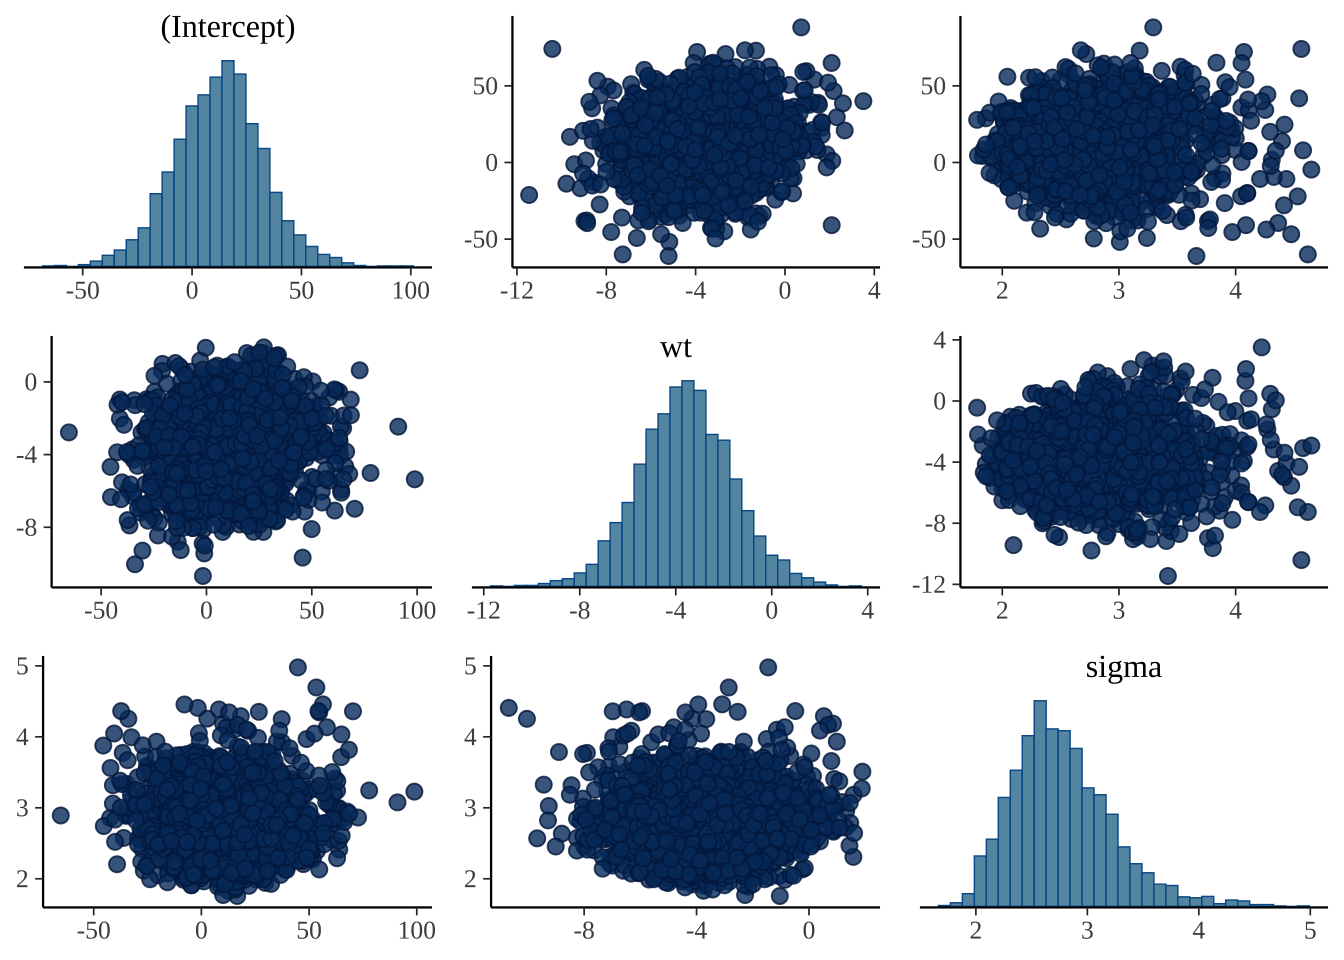
\includegraphics{1001-chapter01_files/figure-latex/unnamed-chunk-25-1} \end{center}

\begin{Shaded}
\begin{Highlighting}[]
\FunctionTok{library}\NormalTok{(RColorBrewer)}
\NormalTok{my\_col }\OtherTok{\textless{}{-}} \FunctionTok{brewer.pal}\NormalTok{(}\DecValTok{3}\NormalTok{, }\StringTok{"RdYlGn"}\NormalTok{)}
\CommentTok{\# brewer.pal(n,name),其中n为颜色的数量,name表示颜色组的名称}
\FunctionTok{plot}\NormalTok{(iris}\SpecialCharTok{$}\NormalTok{Sepal.Length, iris}\SpecialCharTok{$}\NormalTok{Sepal.Width, }\AttributeTok{col =} \FunctionTok{rep}\NormalTok{(my\_col, }\AttributeTok{each =} \DecValTok{50}\NormalTok{))}
\end{Highlighting}
\end{Shaded}

\begin{center}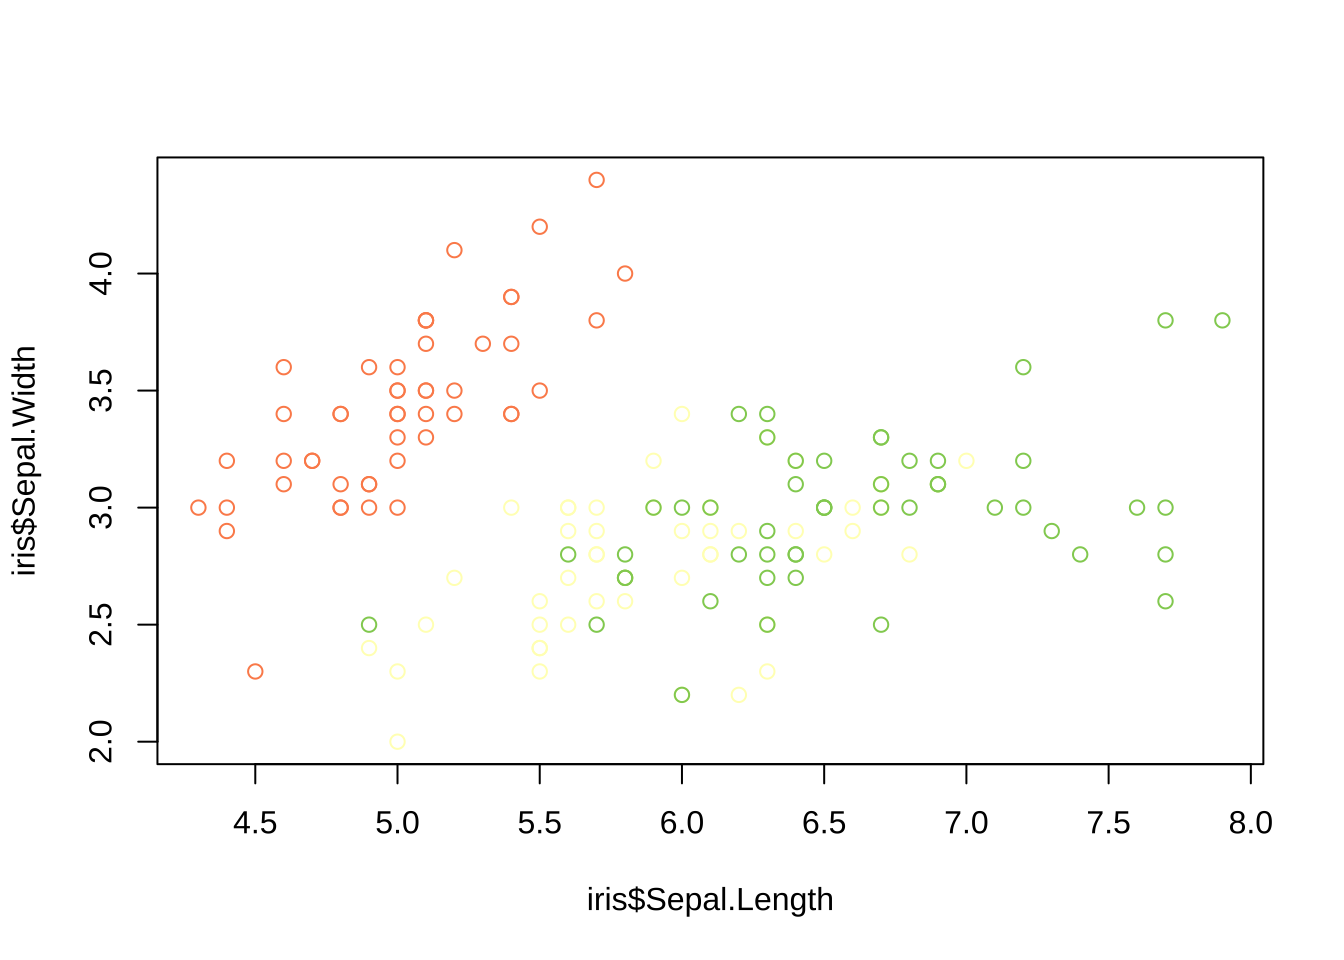
\includegraphics{1001-chapter01_files/figure-latex/unnamed-chunk-26-1} \end{center}

\begin{Shaded}
\begin{Highlighting}[]
\FunctionTok{plot}\NormalTok{(iris}\SpecialCharTok{$}\NormalTok{Sepal.Length, iris}\SpecialCharTok{$}\NormalTok{Sepal.Width, }\AttributeTok{col =} \FunctionTok{rep}\NormalTok{(}\FunctionTok{rainbow}\NormalTok{(}\DecValTok{3}\NormalTok{), }\AttributeTok{each =} \DecValTok{50}\NormalTok{))}
\end{Highlighting}
\end{Shaded}

\begin{center}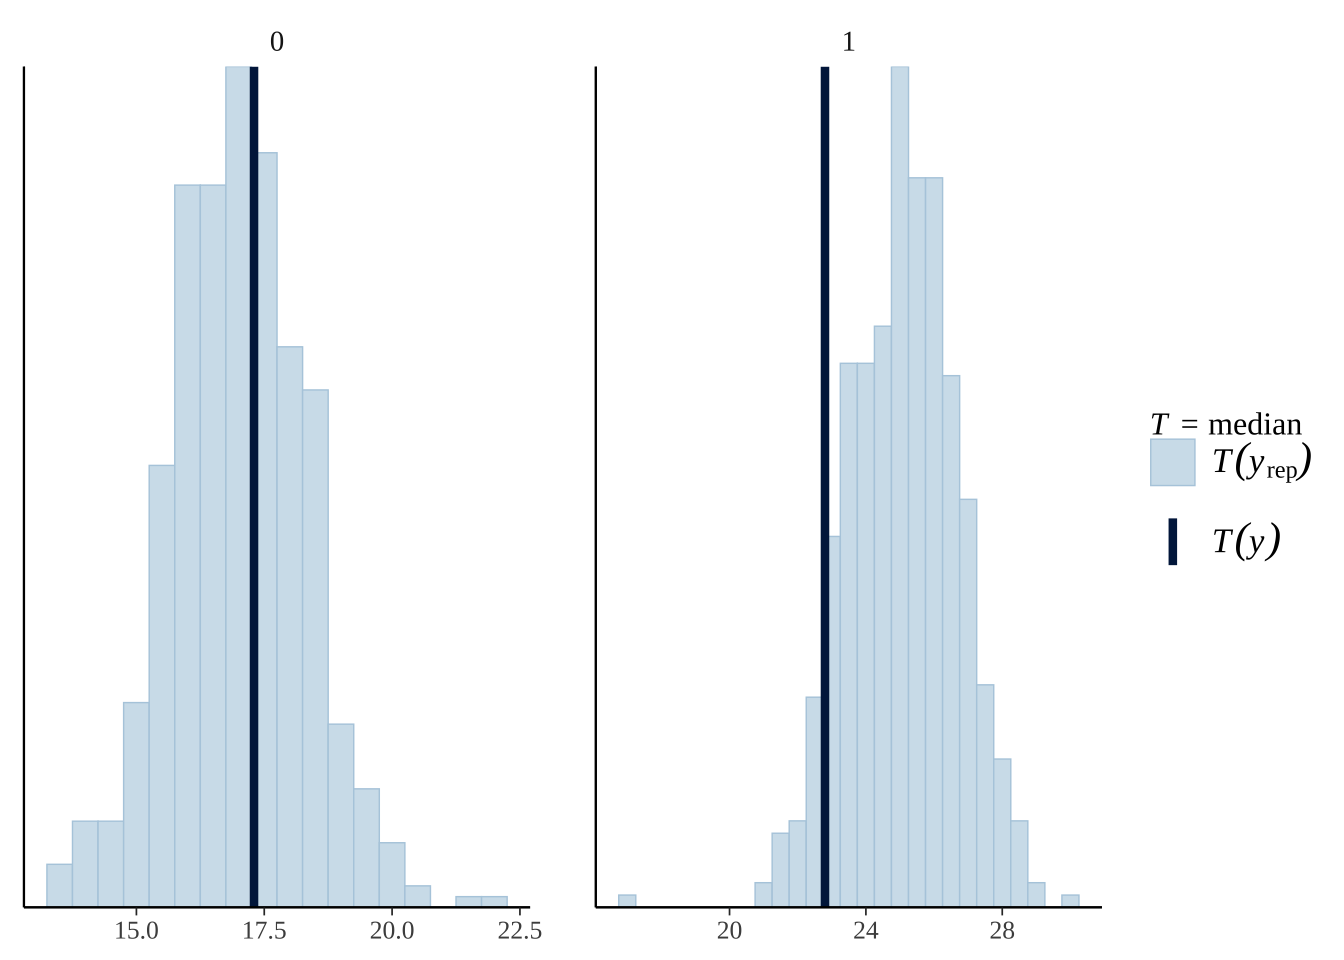
\includegraphics{1001-chapter01_files/figure-latex/unnamed-chunk-26-2} \end{center}

\hypertarget{ux4feeux6539ux70b9ux7b26ux53f7ux4e0eux7ebfux6761}{%
\subsection{修改点符号与线条}\label{ux4feeux6539ux70b9ux7b26ux53f7ux4e0eux7ebfux6761}}

\hypertarget{ux70b9ux6837ux5f0f}{%
\subsubsection{点样式}\label{ux70b9ux6837ux5f0f}}

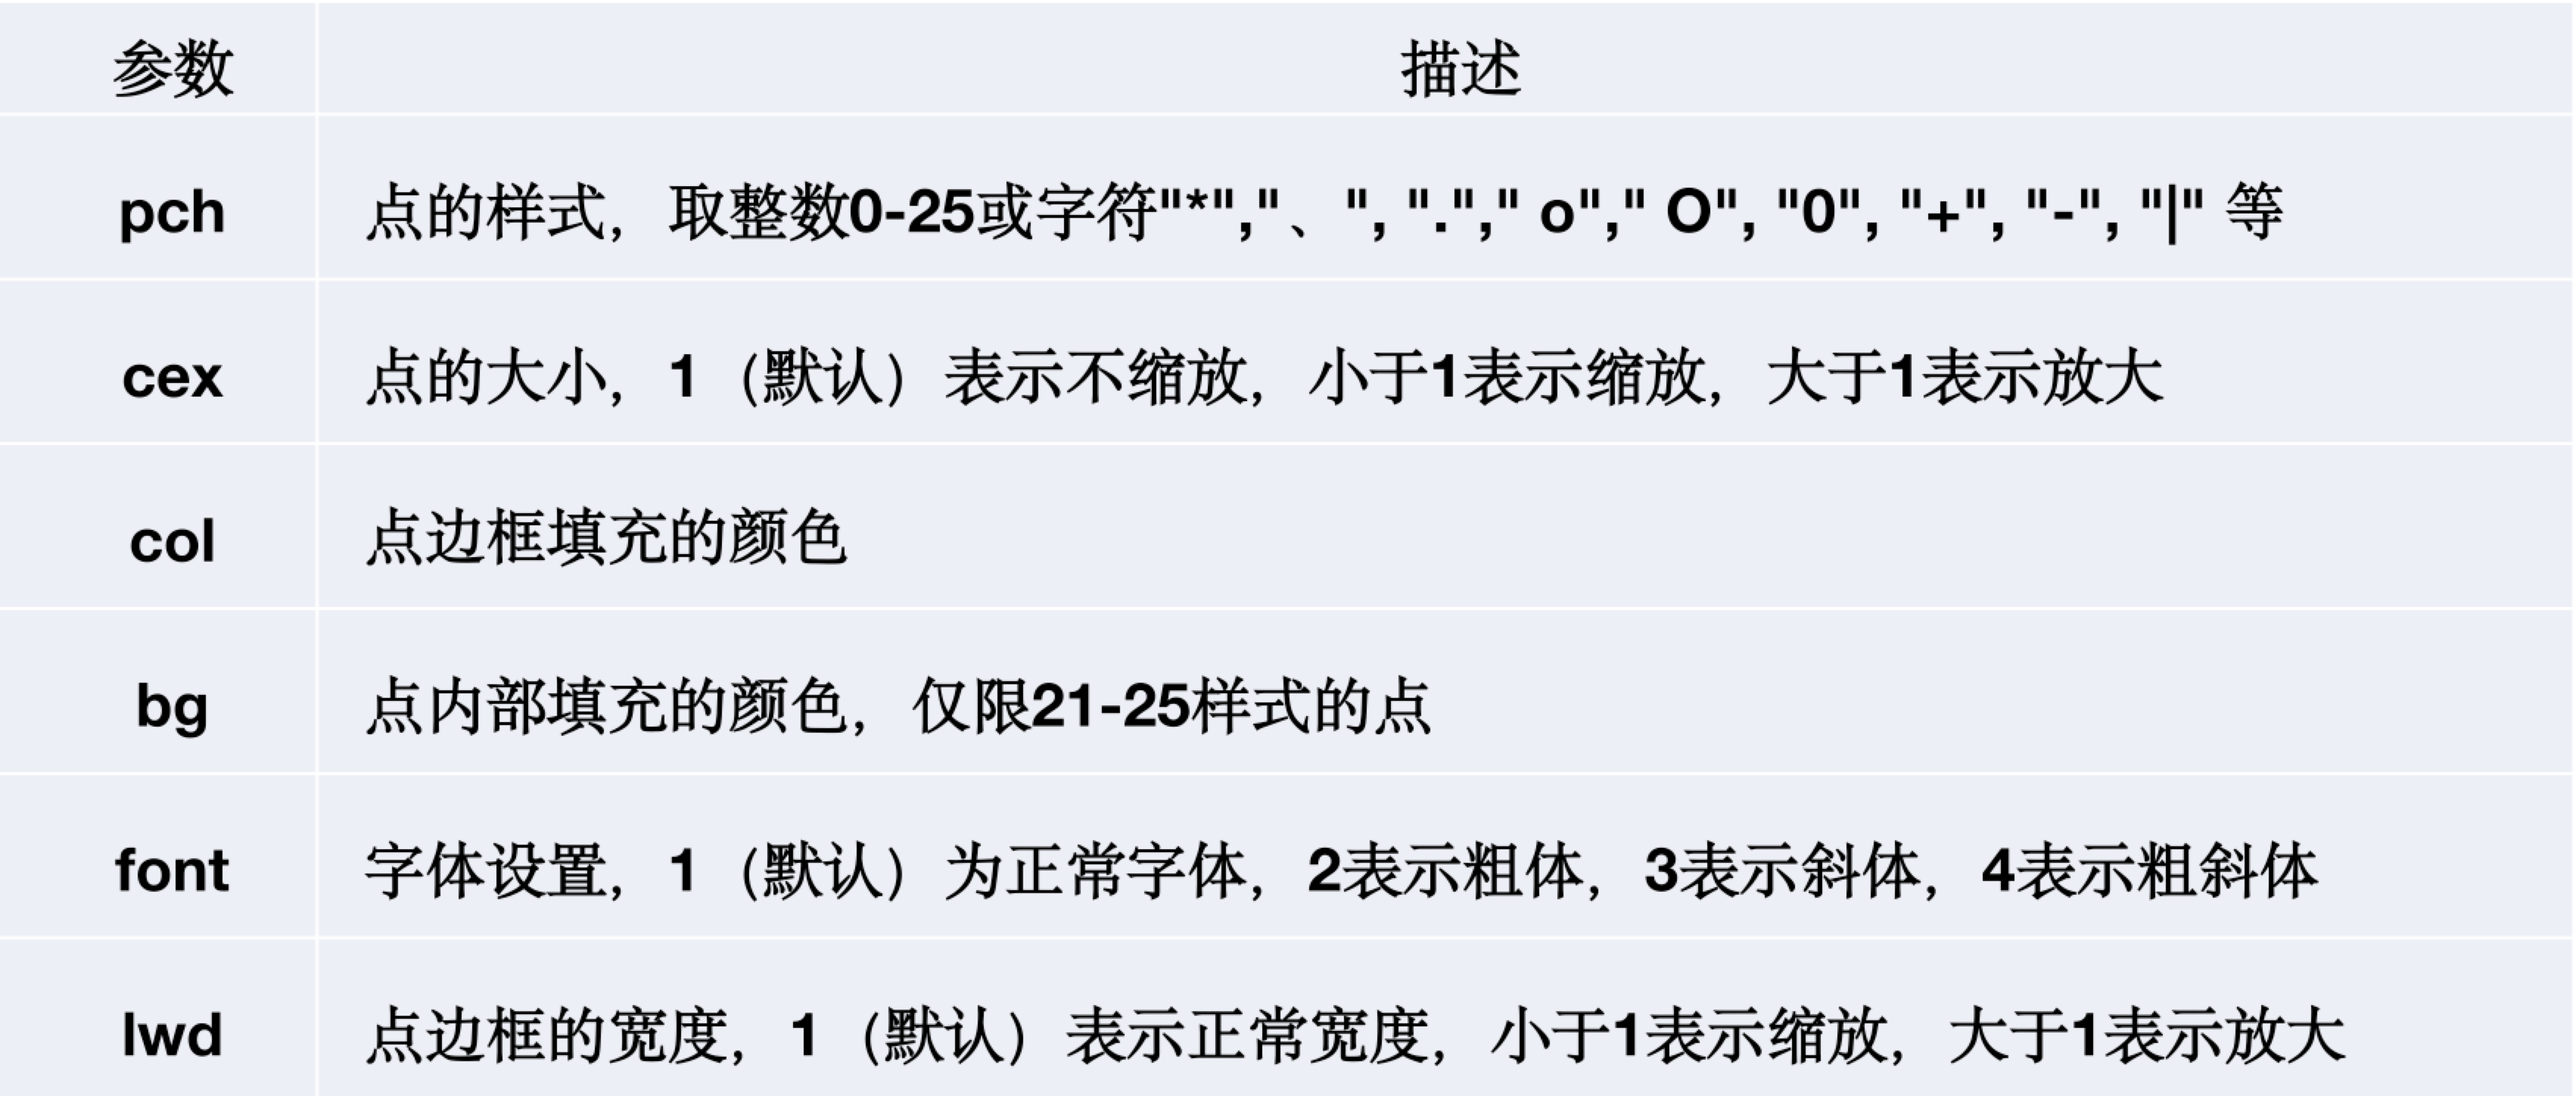
\includegraphics{figure/5.jpg}

\begin{center}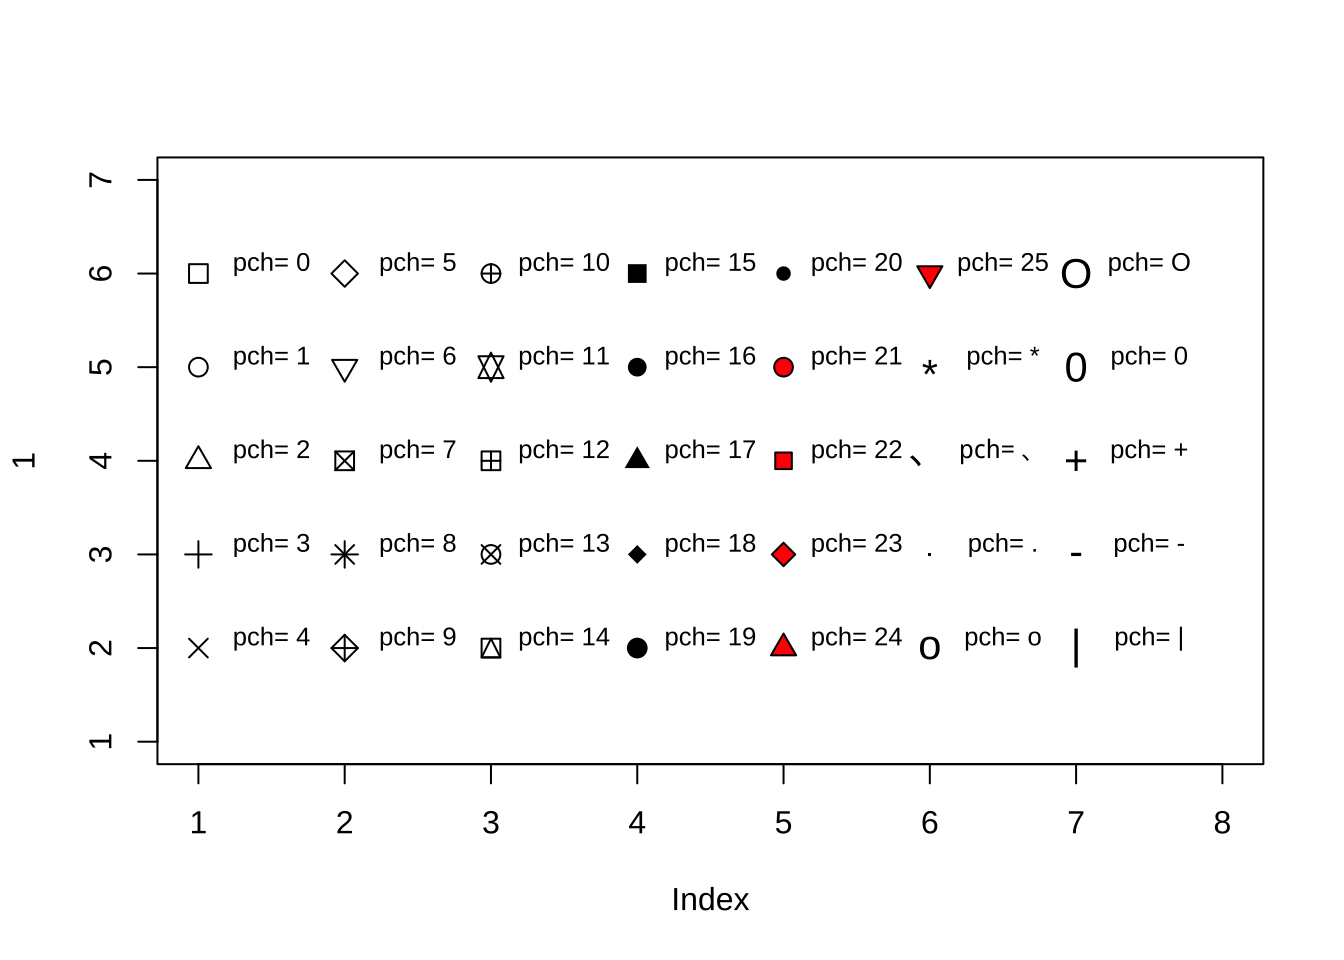
\includegraphics{1001-chapter01_files/figure-latex/unnamed-chunk-27-1} \end{center}

\begin{Shaded}
\begin{Highlighting}[]
\FunctionTok{plot}\NormalTok{(iris}\SpecialCharTok{$}\NormalTok{Sepal.Length, iris}\SpecialCharTok{$}\NormalTok{Sepal.Width, }\AttributeTok{pch =} \FunctionTok{rep}\NormalTok{(}\DecValTok{1}\SpecialCharTok{:}\DecValTok{3}\NormalTok{, }\AttributeTok{each =} \DecValTok{50}\NormalTok{))}
\end{Highlighting}
\end{Shaded}

\begin{center}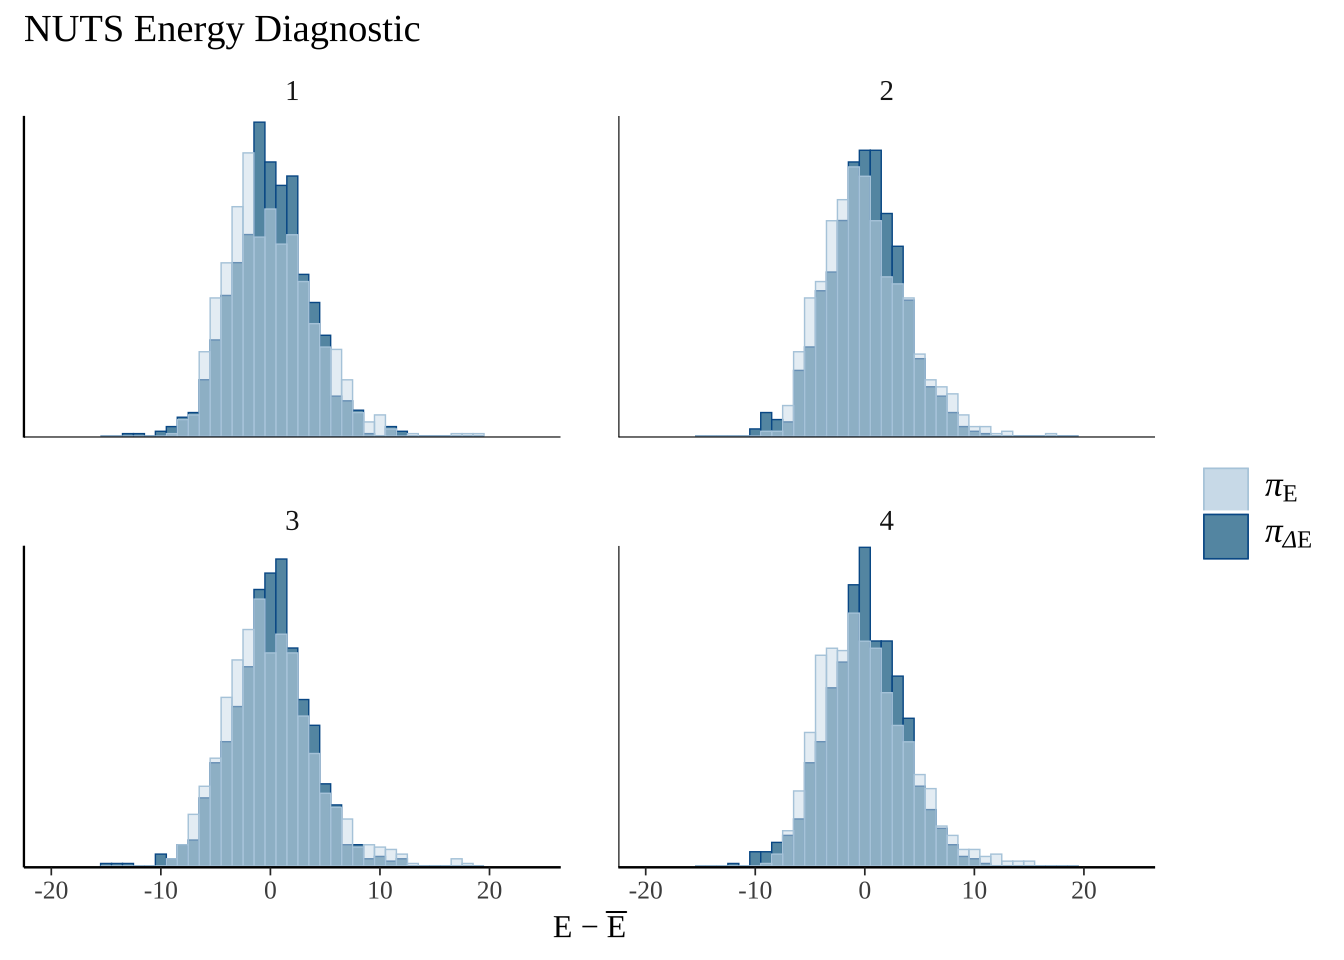
\includegraphics{1001-chapter01_files/figure-latex/unnamed-chunk-28-1} \end{center}

\begin{Shaded}
\begin{Highlighting}[]
\CommentTok{\# plot(1:10,pch=21,cex=1.5,col=\textquotesingle{}red\textquotesingle{},bg = \textquotesingle{}blue\textquotesingle{},lwd=5)}
\end{Highlighting}
\end{Shaded}

\hypertarget{ux7ebfux6761ux6837ux5f0f}{%
\subsubsection{线条样式}\label{ux7ebfux6761ux6837ux5f0f}}

R语言提供了绘制不同类别的线条的多种函数,主要有

\begin{itemize}
\tightlist
\item
  lines:绘制曲线
\item
  abline:绘制直线
\item
  segments:绘制线段
\item
  arrows:在线段加上箭头
\item
  grid:绘制网格线
\end{itemize}

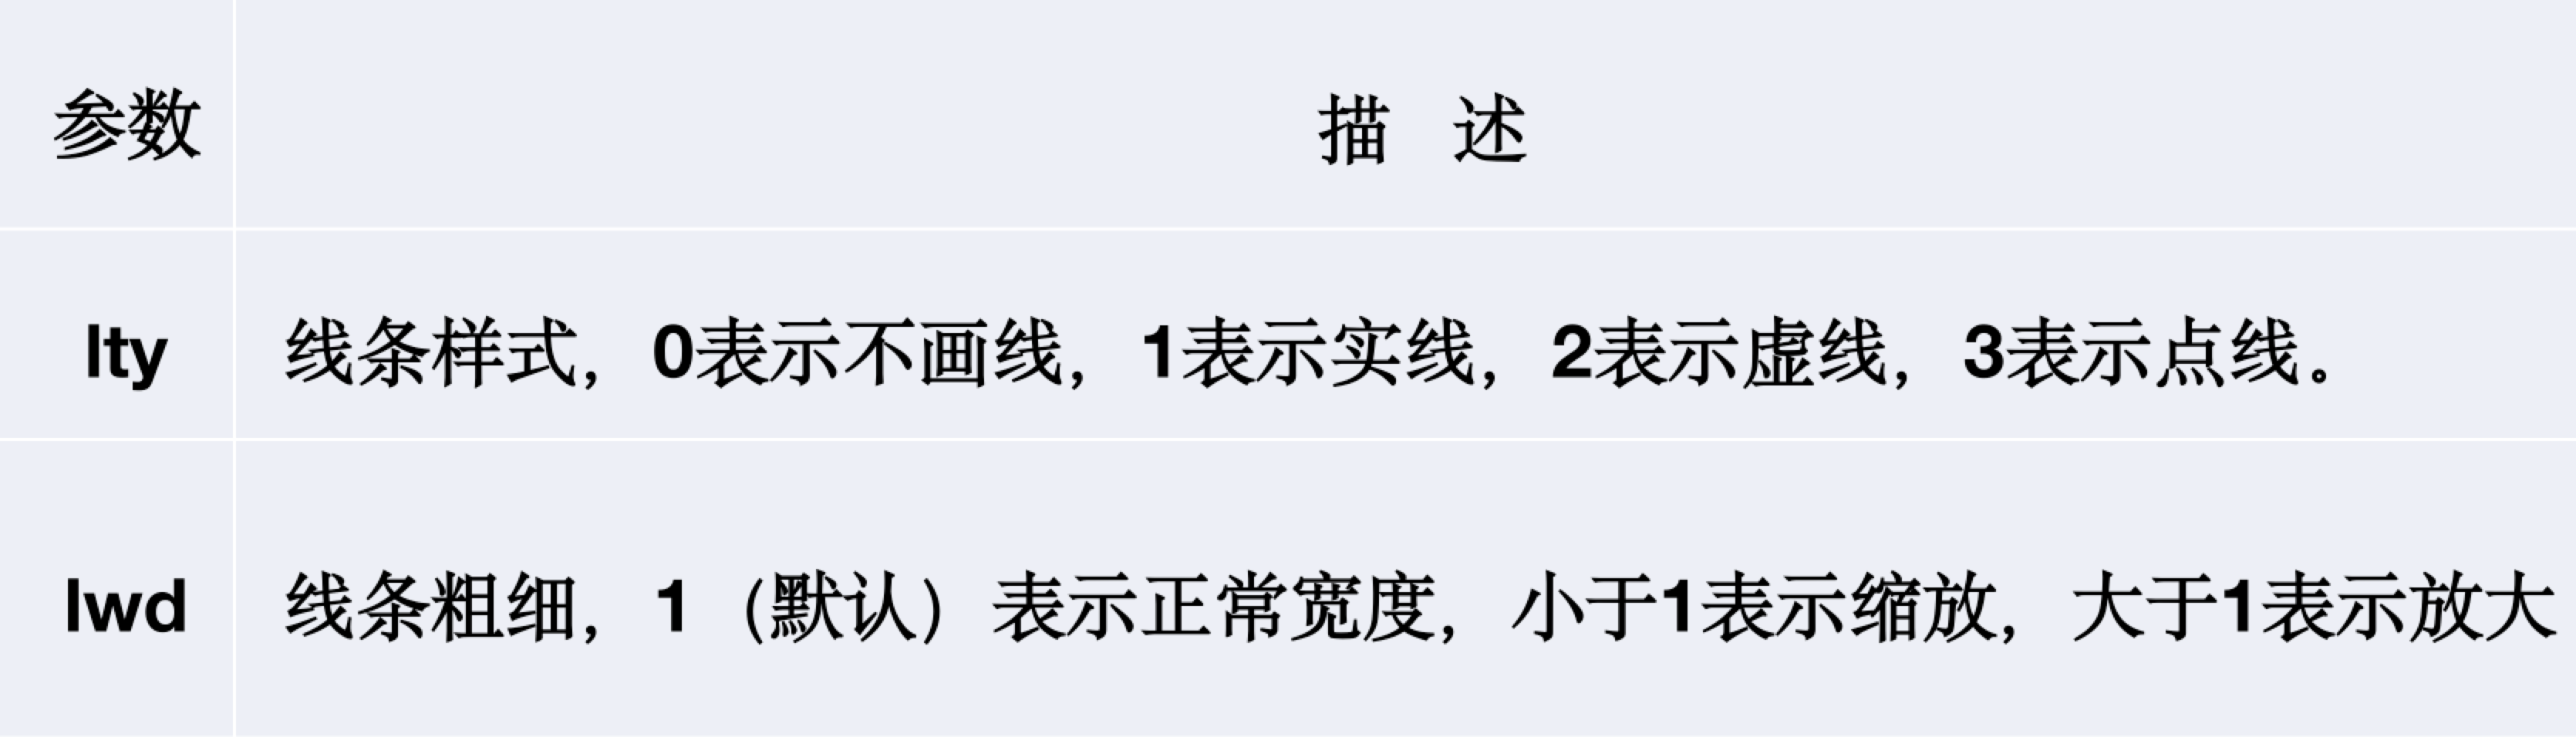
\includegraphics{figure/6.jpg}

以mtcars数据集为例来展示实际绘图过程中线条的应用。

\begin{Shaded}
\begin{Highlighting}[]
\FunctionTok{attach}\NormalTok{(mtcars)}
\NormalTok{smpg }\OtherTok{=}\NormalTok{ (mpg }\SpecialCharTok{{-}} \FunctionTok{min}\NormalTok{(mpg))}\SpecialCharTok{/}\NormalTok{(}\FunctionTok{max}\NormalTok{(mpg) }\SpecialCharTok{{-}} \FunctionTok{min}\NormalTok{(mpg))}
\FunctionTok{plot}\NormalTok{(wt, smpg, }\AttributeTok{ylab =} \StringTok{"standardized mpg"}\NormalTok{)}
\CommentTok{\# 添加核密度曲线图}
\FunctionTok{lines}\NormalTok{(}\FunctionTok{density}\NormalTok{(wt), }\AttributeTok{col =} \StringTok{"red"}\NormalTok{)}
\CommentTok{\# 指向密度曲线的箭头}
\FunctionTok{arrows}\NormalTok{(}\FloatTok{1.8}\NormalTok{, }\FloatTok{0.05}\NormalTok{, }\FloatTok{1.5}\NormalTok{, }\FloatTok{0.1}\NormalTok{)}
\FunctionTok{text}\NormalTok{(}\DecValTok{2}\NormalTok{, }\FloatTok{0.05}\NormalTok{, }\StringTok{"density curve"}\NormalTok{, }\AttributeTok{cex =} \FloatTok{0.6}\NormalTok{)}
\CommentTok{\# 添加回归线}
\FunctionTok{abline}\NormalTok{(}\FunctionTok{lm}\NormalTok{(smpg }\SpecialCharTok{\textasciitilde{}}\NormalTok{ wt), }\AttributeTok{lty =} \DecValTok{2}\NormalTok{, }\AttributeTok{col =} \StringTok{"green"}\NormalTok{)}
\CommentTok{\# 指向回归直线的箭头}
\FunctionTok{arrows}\NormalTok{(}\DecValTok{2}\NormalTok{, }\FloatTok{0.5}\NormalTok{, }\DecValTok{2}\NormalTok{, }\FloatTok{0.7}\NormalTok{, }\AttributeTok{angle =} \DecValTok{10}\NormalTok{, }\AttributeTok{cex =} \FloatTok{0.5}\NormalTok{)}
\FunctionTok{text}\NormalTok{(}\DecValTok{2}\NormalTok{, }\FloatTok{0.45}\NormalTok{, }\StringTok{"regression line"}\NormalTok{, }\AttributeTok{cex =} \FloatTok{0.6}\NormalTok{)}
\CommentTok{\# wt与mpg反向线性相关,添加最大最小值线段表现这种关系}
\FunctionTok{segments}\NormalTok{(}\FunctionTok{min}\NormalTok{(wt), }\FunctionTok{max}\NormalTok{(smpg), }\FunctionTok{max}\NormalTok{(wt), }\FunctionTok{min}\NormalTok{(smpg), }\AttributeTok{lty =} \DecValTok{3}\NormalTok{, }\AttributeTok{col =} \StringTok{"blue"}\NormalTok{)}
\CommentTok{\# 指向最大最小值线段的箭头}
\FunctionTok{arrows}\NormalTok{(}\DecValTok{3}\NormalTok{, }\FloatTok{0.8}\NormalTok{, }\FloatTok{2.5}\NormalTok{, }\FloatTok{0.76}\NormalTok{, }\AttributeTok{angle =} \DecValTok{10}\NormalTok{, }\AttributeTok{cex =} \FloatTok{0.5}\NormalTok{)}
\FunctionTok{text}\NormalTok{(}\FloatTok{3.3}\NormalTok{, }\FloatTok{0.8}\NormalTok{, }\StringTok{"line segments"}\NormalTok{, }\AttributeTok{cex =} \FloatTok{0.6}\NormalTok{)}
\CommentTok{\# 添加网格线作为背景}
\FunctionTok{grid}\NormalTok{(}\AttributeTok{nx =} \DecValTok{4}\NormalTok{, }\AttributeTok{ny =} \DecValTok{5}\NormalTok{, }\AttributeTok{lty =} \DecValTok{2}\NormalTok{, }\AttributeTok{col =} \StringTok{"grey"}\NormalTok{)}
\end{Highlighting}
\end{Shaded}

\begin{center}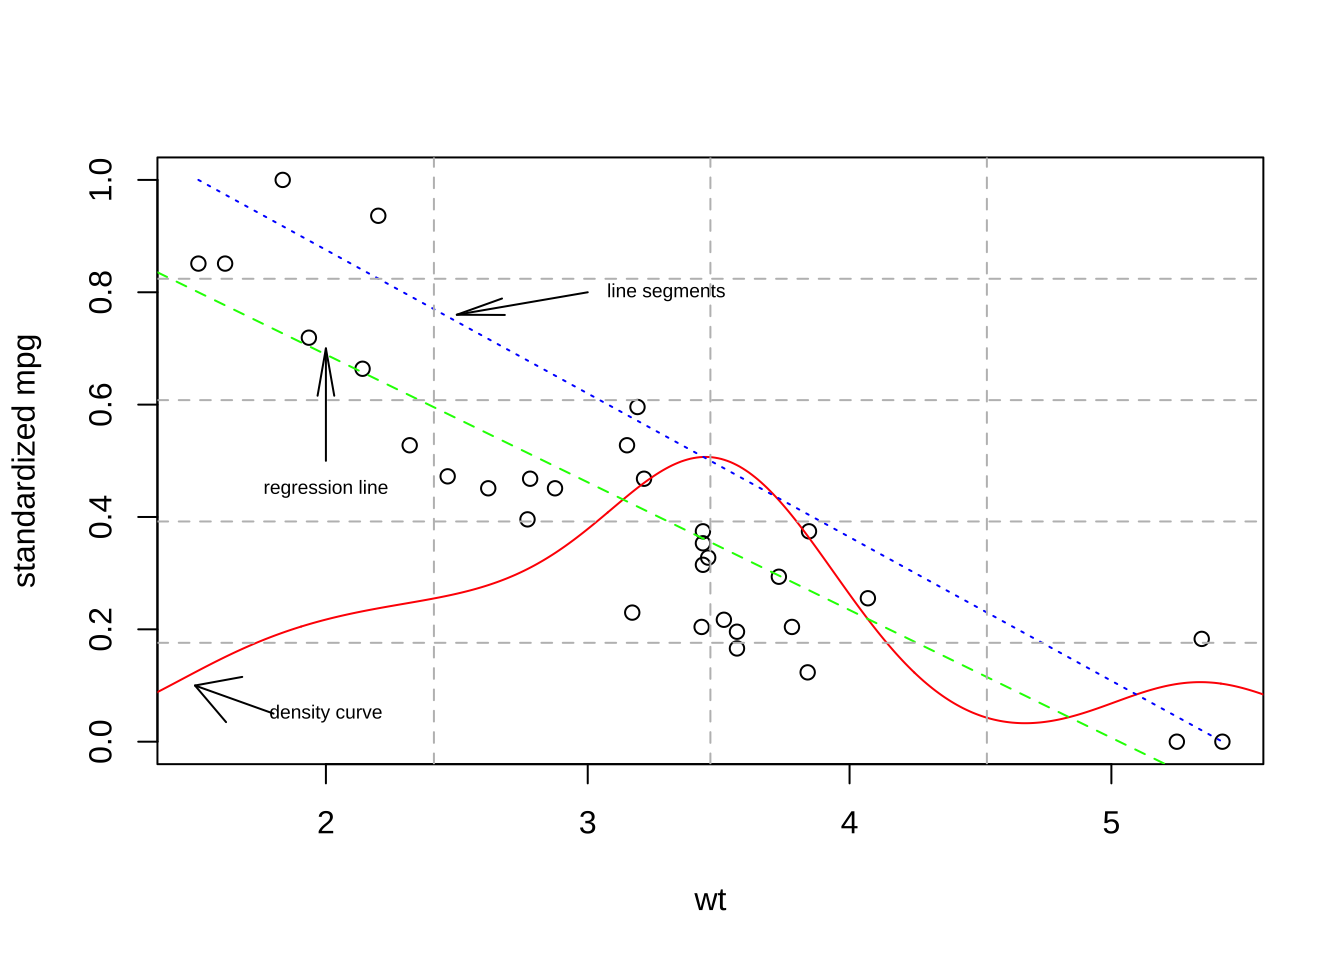
\includegraphics{1001-chapter01_files/figure-latex/unnamed-chunk-29-1} \end{center}

\hypertarget{ux4feeux6539ux6587ux672cux53c2ux6570}{%
\subsubsection{修改文本参数}\label{ux4feeux6539ux6587ux672cux53c2ux6570}}

title、text和mtext函数可以在打开的画布上添加文字元素。

\begin{itemize}
\tightlist
\item
  title可以添加标题元素;
\item
  text可以任意位置添加文本;
\item
  mtext函数则是在四条边上添加文本。
\end{itemize}

\begin{Shaded}
\begin{Highlighting}[]
\FunctionTok{par}\NormalTok{(}\AttributeTok{mfrow =} \FunctionTok{c}\NormalTok{(}\DecValTok{2}\NormalTok{, }\DecValTok{2}\NormalTok{))}
\CommentTok{\# 图一:图形添加标题}
\FunctionTok{plot}\NormalTok{(}\FunctionTok{c}\NormalTok{(}\DecValTok{0}\SpecialCharTok{:}\DecValTok{5}\NormalTok{), }\AttributeTok{col =} \StringTok{"red"}\NormalTok{, }\AttributeTok{xlab =} \StringTok{""}\NormalTok{, }\AttributeTok{ylab =} \StringTok{""}\NormalTok{)}
\FunctionTok{title}\NormalTok{(}\AttributeTok{main =} \FunctionTok{list}\NormalTok{(}\StringTok{"主标题"}\NormalTok{, }\AttributeTok{cex =} \FloatTok{1.5}\NormalTok{), }\AttributeTok{sub =} \FunctionTok{list}\NormalTok{(}\StringTok{"副标题"}\NormalTok{, }\AttributeTok{cex =} \FloatTok{1.2}\NormalTok{), }\AttributeTok{xlab =} \StringTok{"x轴标题"}\NormalTok{, }
    \AttributeTok{ylab =} \StringTok{"y轴标题"}\NormalTok{)}
\CommentTok{\# 图二:图形周边添加文本}
\FunctionTok{plot}\NormalTok{(}\FunctionTok{c}\NormalTok{(}\DecValTok{0}\SpecialCharTok{:}\DecValTok{5}\NormalTok{), }\AttributeTok{col =} \StringTok{"white"}\NormalTok{)}
\FunctionTok{mtext}\NormalTok{(}\StringTok{"side=1:下边"}\NormalTok{, }\AttributeTok{side =} \DecValTok{1}\NormalTok{, }\AttributeTok{line =} \DecValTok{2}\NormalTok{)}
\FunctionTok{mtext}\NormalTok{(}\StringTok{"side=2:左边"}\NormalTok{, }\AttributeTok{side =} \DecValTok{2}\NormalTok{, }\AttributeTok{line =} \DecValTok{2}\NormalTok{)}
\FunctionTok{mtext}\NormalTok{(}\StringTok{"side=3:上边"}\NormalTok{, }\AttributeTok{side =} \DecValTok{3}\NormalTok{)}
\FunctionTok{mtext}\NormalTok{(}\StringTok{"side=4:右边"}\NormalTok{, }\AttributeTok{side =} \DecValTok{4}\NormalTok{)}
\CommentTok{\# 图三:字体展示}
\FunctionTok{plot}\NormalTok{(}\FunctionTok{c}\NormalTok{(}\DecValTok{0}\SpecialCharTok{:}\DecValTok{5}\NormalTok{), }\AttributeTok{col =} \StringTok{"white"}\NormalTok{)}
\FunctionTok{text}\NormalTok{(}\DecValTok{2}\NormalTok{, }\DecValTok{4}\NormalTok{, }\AttributeTok{labels =} \StringTok{"font=1:正常字体(默认)"}\NormalTok{, }\AttributeTok{font =} \DecValTok{1}\NormalTok{)}
\FunctionTok{text}\NormalTok{(}\DecValTok{3}\NormalTok{, }\DecValTok{3}\NormalTok{, }\AttributeTok{labels =} \StringTok{"font=2:粗体字体"}\NormalTok{, }\AttributeTok{font =} \DecValTok{2}\NormalTok{)}
\FunctionTok{text}\NormalTok{(}\DecValTok{4}\NormalTok{, }\DecValTok{2}\NormalTok{, }\AttributeTok{labels =} \StringTok{"font=3:斜体字体"}\NormalTok{, }\AttributeTok{font =} \DecValTok{3}\NormalTok{)}
\FunctionTok{text}\NormalTok{(}\DecValTok{5}\NormalTok{, }\DecValTok{1}\NormalTok{, }\AttributeTok{labels =} \StringTok{"font=4:粗斜体字体"}\NormalTok{, }\AttributeTok{font =} \DecValTok{4}\NormalTok{)}
\CommentTok{\# 图四:字体大小展示}
\FunctionTok{plot}\NormalTok{(}\FunctionTok{c}\NormalTok{(}\DecValTok{0}\SpecialCharTok{:}\DecValTok{6}\NormalTok{), }\AttributeTok{col =} \StringTok{"white"}\NormalTok{, }\AttributeTok{xlim =} \FunctionTok{c}\NormalTok{(}\DecValTok{1}\NormalTok{, }\DecValTok{8}\NormalTok{))}
\FunctionTok{text}\NormalTok{(}\DecValTok{2}\NormalTok{, }\DecValTok{5}\NormalTok{, }\AttributeTok{labels =} \StringTok{"cex=0.5:放大0.5倍"}\NormalTok{, }\AttributeTok{cex =} \FloatTok{0.5}\NormalTok{)}
\FunctionTok{text}\NormalTok{(}\DecValTok{3}\NormalTok{, }\DecValTok{4}\NormalTok{, }\AttributeTok{labels =} \StringTok{"cex=0.8:放大0.8倍"}\NormalTok{, }\AttributeTok{cex =} \FloatTok{0.8}\NormalTok{)}
\FunctionTok{text}\NormalTok{(}\DecValTok{4}\NormalTok{, }\DecValTok{3}\NormalTok{, }\AttributeTok{labels =} \StringTok{"cex=1(默认):正常大小"}\NormalTok{, }\AttributeTok{cex =} \DecValTok{1}\NormalTok{)}
\FunctionTok{text}\NormalTok{(}\DecValTok{5}\NormalTok{, }\DecValTok{2}\NormalTok{, }\AttributeTok{labels =} \StringTok{"cex=1.2:放大1.2倍"}\NormalTok{, }\AttributeTok{cex =} \FloatTok{1.2}\NormalTok{)}
\FunctionTok{text}\NormalTok{(}\DecValTok{6}\NormalTok{, }\DecValTok{1}\NormalTok{, }\AttributeTok{labels =} \StringTok{"cex=1.5:放大1.5倍"}\NormalTok{, }\AttributeTok{cex =} \FloatTok{1.5}\NormalTok{)}
\end{Highlighting}
\end{Shaded}

\begin{center}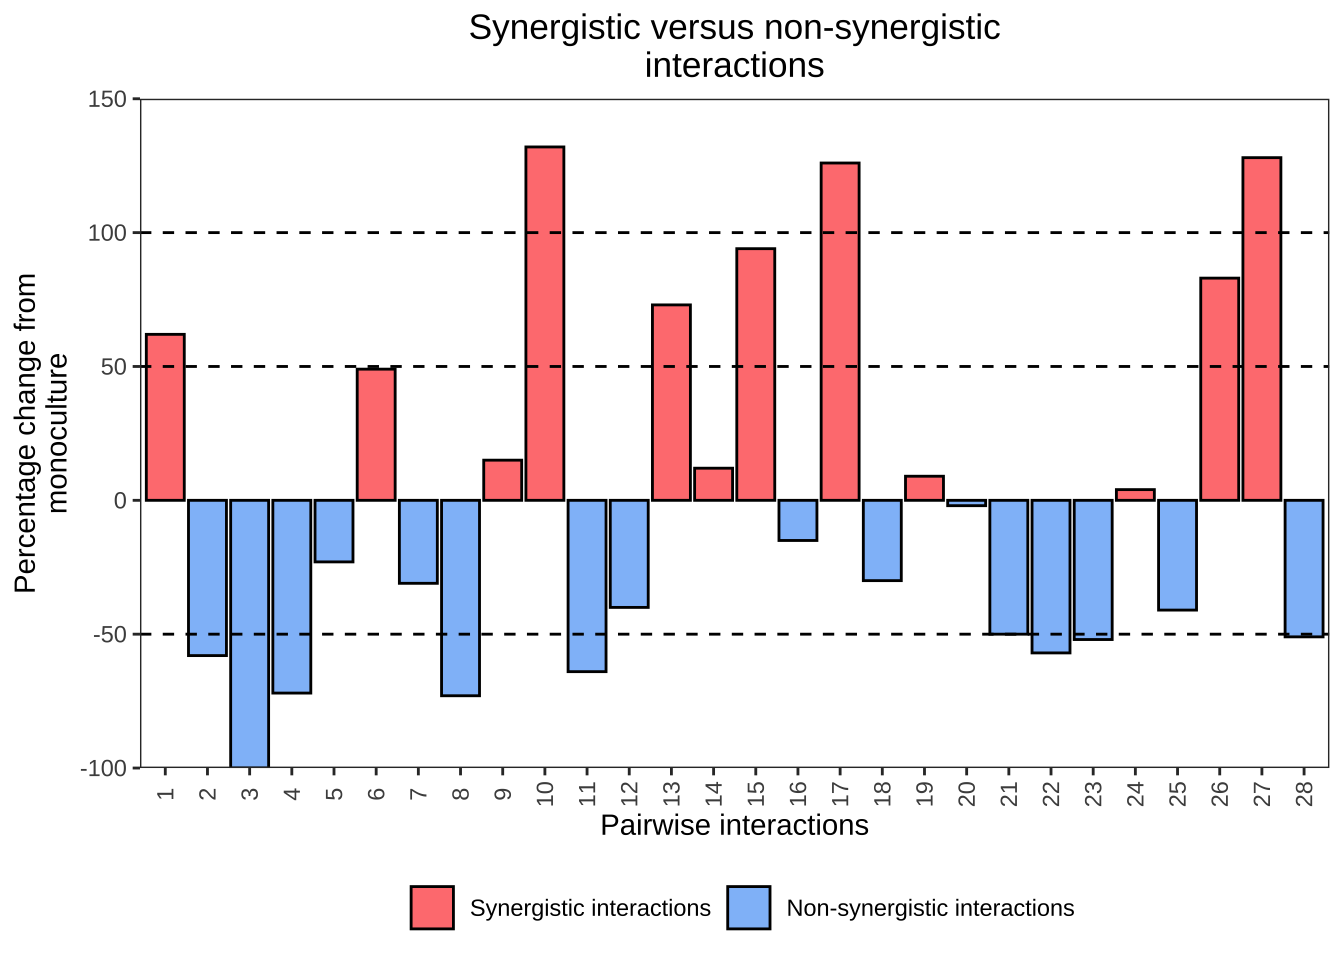
\includegraphics{1001-chapter01_files/figure-latex/unnamed-chunk-30-1} \end{center}

\textbf{例子}:

\begin{Shaded}
\begin{Highlighting}[]
\FunctionTok{attach}\NormalTok{(mtcars)}
\FunctionTok{plot}\NormalTok{(wt, mpg, }\AttributeTok{xlab =} \StringTok{"Weight (1000 lbs)"}\NormalTok{, }\AttributeTok{ylab =} \StringTok{"Miles/(US) gallon"}\NormalTok{)  }\CommentTok{\#绘图,并修改x,y轴的标题}
\FunctionTok{title}\NormalTok{(}\AttributeTok{main =} \FunctionTok{list}\NormalTok{(}\StringTok{"mtcars wt V.S. mpg"}\NormalTok{, }\AttributeTok{cex =} \FloatTok{1.5}\NormalTok{))  }\CommentTok{\# 添加标题}
\FunctionTok{text}\NormalTok{(}\FloatTok{4.5}\NormalTok{, }\DecValTok{34}\NormalTok{, }\AttributeTok{labels =} \StringTok{"extracted from the 1974"}\NormalTok{, }\AttributeTok{cex =} \FloatTok{1.5}\NormalTok{)  }\CommentTok{\# 说明数据来源}
\FunctionTok{text}\NormalTok{(}\FloatTok{4.5}\NormalTok{, }\DecValTok{32}\NormalTok{, }\AttributeTok{labels =} \StringTok{"Motor Trend US"}\NormalTok{, }\AttributeTok{font =} \DecValTok{3}\NormalTok{)  }\CommentTok{\# 杂志名称}
\end{Highlighting}
\end{Shaded}

\begin{center}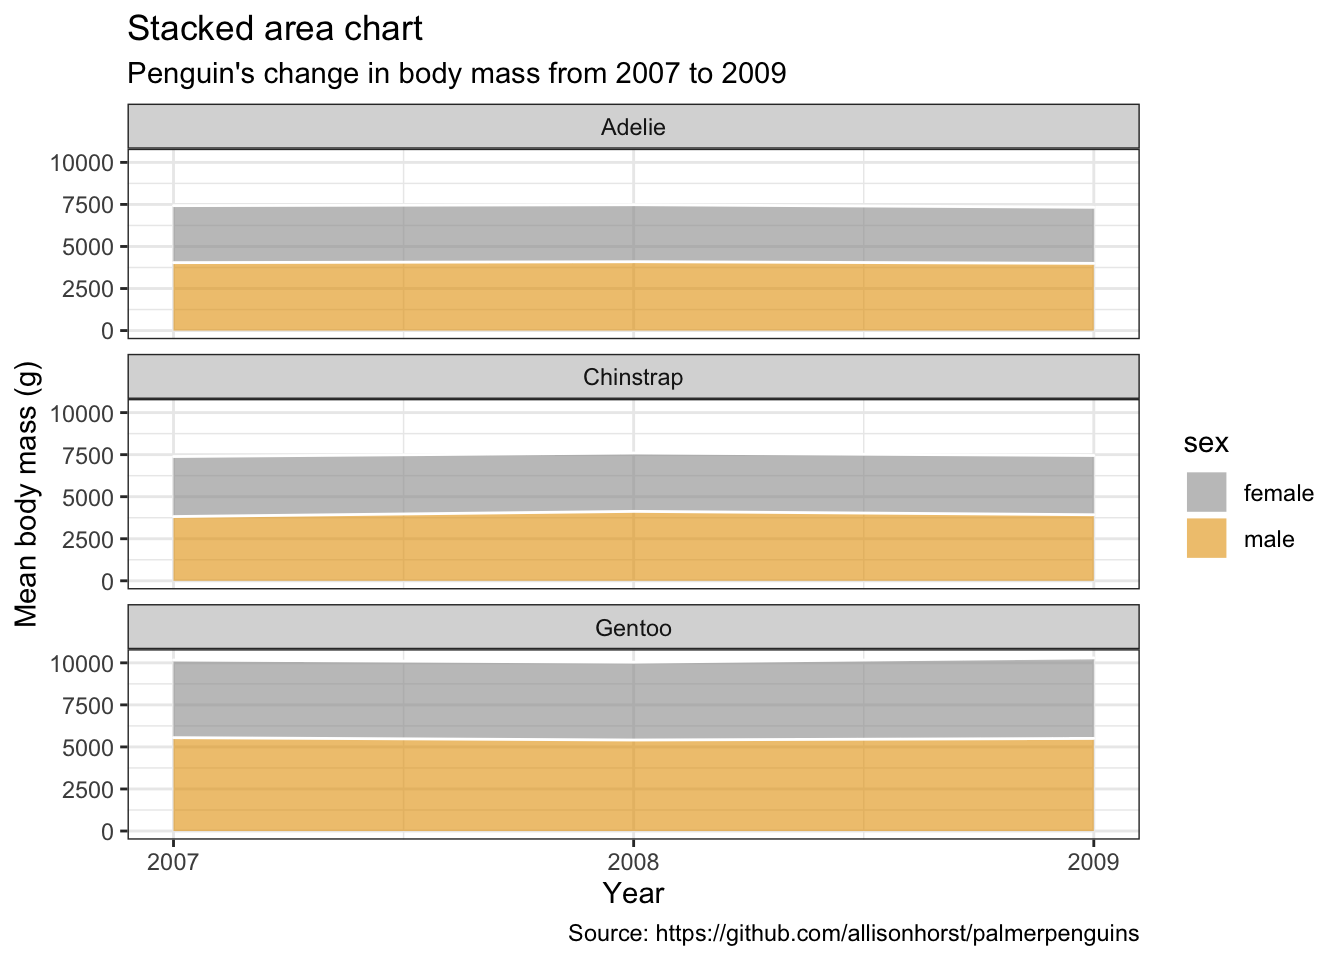
\includegraphics{1001-chapter01_files/figure-latex/unnamed-chunk-31-1} \end{center}

\hypertarget{ux8bbeux7f6eux5750ux6807ux8f74}{%
\subsubsection{设置坐标轴}\label{ux8bbeux7f6eux5750ux6807ux8f74}}

使用\texttt{axis()}进行设置坐标轴。


\includegraphics{figure/7.jpg}

\begin{Shaded}
\begin{Highlighting}[]
\FunctionTok{plot}\NormalTok{(}\FunctionTok{c}\NormalTok{(}\DecValTok{1}\SpecialCharTok{:}\DecValTok{12}\NormalTok{), }\AttributeTok{col =} \StringTok{"white"}\NormalTok{, }\AttributeTok{xaxt =} \StringTok{"n"}\NormalTok{, }\AttributeTok{yaxt =} \StringTok{"n"}\NormalTok{, }\AttributeTok{ann =} \ConstantTok{FALSE}\NormalTok{)}
\FunctionTok{axis}\NormalTok{(}\DecValTok{1}\NormalTok{, }\AttributeTok{at =} \DecValTok{1}\SpecialCharTok{:}\DecValTok{12}\NormalTok{, }\AttributeTok{col.axis =} \StringTok{"red"}\NormalTok{, }\AttributeTok{labels =}\NormalTok{ month.abb)}
\FunctionTok{axis}\NormalTok{(}\DecValTok{2}\NormalTok{, }\AttributeTok{at =} \FunctionTok{seq}\NormalTok{(}\DecValTok{1}\NormalTok{, }\DecValTok{12}\NormalTok{, }\AttributeTok{length =} \DecValTok{10}\NormalTok{), }\AttributeTok{col.axis =} \StringTok{"red"}\NormalTok{, }\AttributeTok{labels =} \DecValTok{1}\SpecialCharTok{:}\DecValTok{10}\NormalTok{, }\AttributeTok{las =} \DecValTok{2}\NormalTok{)}
\FunctionTok{axis}\NormalTok{(}\DecValTok{3}\NormalTok{, }\AttributeTok{at =} \FunctionTok{seq}\NormalTok{(}\DecValTok{1}\NormalTok{, }\DecValTok{12}\NormalTok{, }\AttributeTok{length =} \DecValTok{7}\NormalTok{), }\AttributeTok{col.axis =} \StringTok{"blue"}\NormalTok{, }\AttributeTok{cex.axis =} \FloatTok{0.7}\NormalTok{, }\AttributeTok{tck =} \SpecialCharTok{{-}}\FloatTok{0.01}\NormalTok{, }
    \AttributeTok{labels =} \FunctionTok{c}\NormalTok{(}\StringTok{"Mon"}\NormalTok{, }\StringTok{"Tues"}\NormalTok{, }\StringTok{"Wed"}\NormalTok{, }\StringTok{"Thu"}\NormalTok{, }\StringTok{"Fri"}\NormalTok{, }\StringTok{"Sat"}\NormalTok{, }\StringTok{"Sun"}\NormalTok{))}
\FunctionTok{axis}\NormalTok{(}\DecValTok{4}\NormalTok{, }\AttributeTok{at =} \FunctionTok{seq}\NormalTok{(}\DecValTok{1}\NormalTok{, }\DecValTok{12}\NormalTok{, }\AttributeTok{length =} \DecValTok{11}\NormalTok{), }\AttributeTok{col.axis =} \StringTok{"blue"}\NormalTok{, }\AttributeTok{cex.axis =} \FloatTok{0.7}\NormalTok{, }\AttributeTok{tck =} \SpecialCharTok{{-}}\FloatTok{0.01}\NormalTok{, }
    \AttributeTok{labels =} \FunctionTok{seq}\NormalTok{(}\DecValTok{0}\NormalTok{, }\DecValTok{1}\NormalTok{, }\FloatTok{0.1}\NormalTok{), }\AttributeTok{las =} \DecValTok{2}\NormalTok{)}
\end{Highlighting}
\end{Shaded}

\begin{center}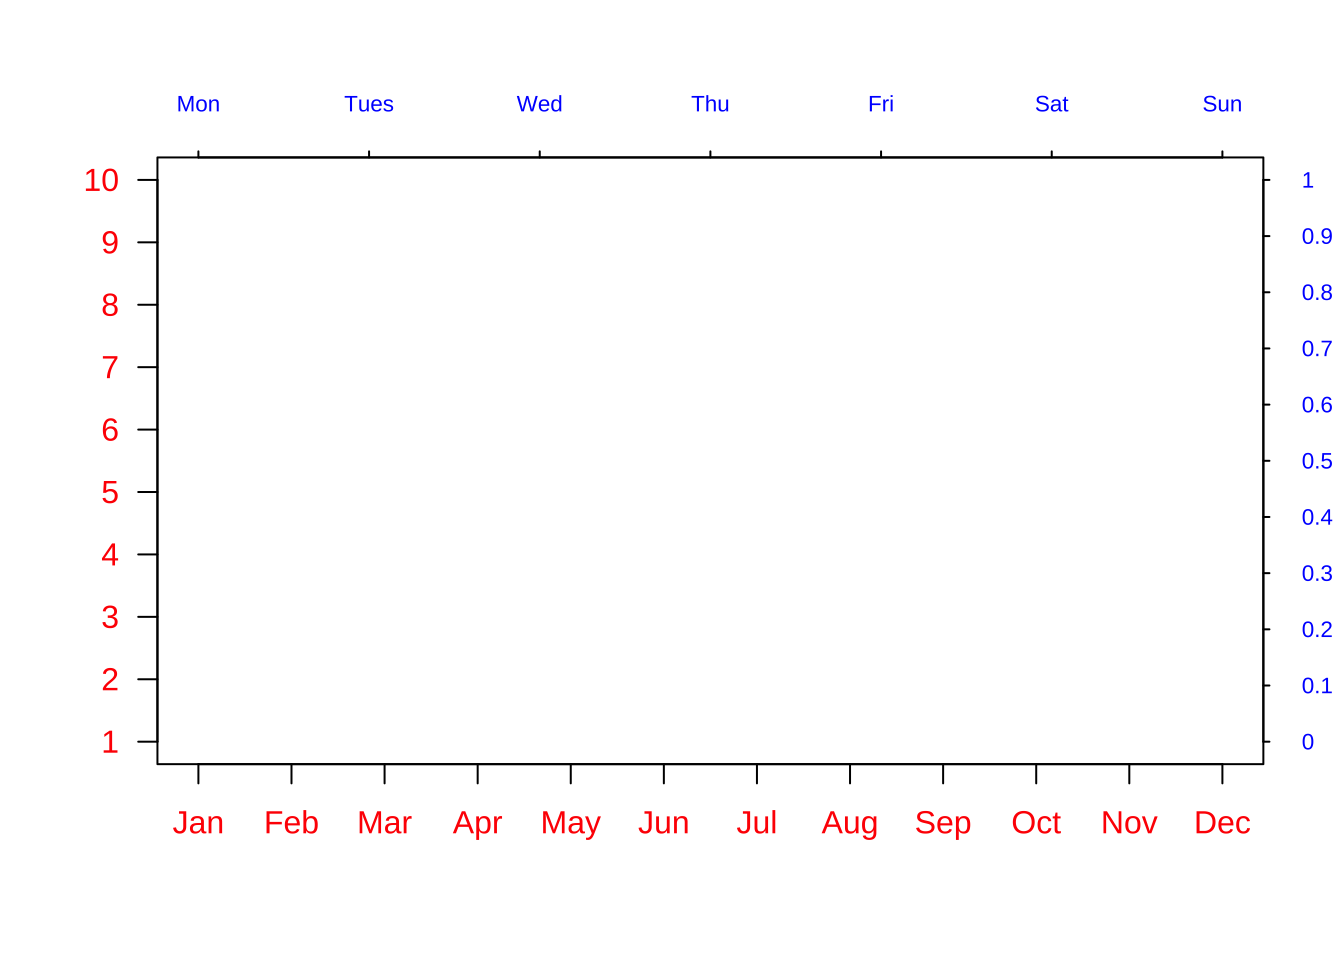
\includegraphics{1001-chapter01_files/figure-latex/unnamed-chunk-32-1} \end{center}

\hypertarget{ux6dfbux52a0ux56feux4f8b}{%
\subsubsection{添加图例}\label{ux6dfbux52a0ux56feux4f8b}}

legend函数的绘制图例的位置效果

\begin{Shaded}
\begin{Highlighting}[]
\NormalTok{local }\OtherTok{=} \FunctionTok{c}\NormalTok{(}\StringTok{"bottomright"}\NormalTok{, }\StringTok{"bottom"}\NormalTok{, }\StringTok{"bottomleft"}\NormalTok{, }\StringTok{"left"}\NormalTok{, }\StringTok{"topleft"}\NormalTok{, }\StringTok{"top"}\NormalTok{, }\StringTok{"topright"}\NormalTok{, }
    \StringTok{"right"}\NormalTok{, }\StringTok{"center"}\NormalTok{)}
\FunctionTok{par}\NormalTok{(}\AttributeTok{mar =} \FunctionTok{c}\NormalTok{(}\DecValTok{4}\NormalTok{, }\DecValTok{2}\NormalTok{, }\DecValTok{4}\NormalTok{, }\DecValTok{2}\NormalTok{), }\AttributeTok{pty =} \StringTok{"m"}\NormalTok{)}
\FunctionTok{plot}\NormalTok{(}\FunctionTok{c}\NormalTok{(}\DecValTok{0}\SpecialCharTok{:}\DecValTok{10}\NormalTok{), }\AttributeTok{col =} \StringTok{"white"}\NormalTok{)}
\FunctionTok{legend}\NormalTok{(}\DecValTok{3}\NormalTok{, }\DecValTok{8}\NormalTok{, }\StringTok{"图例在(3,8)"}\NormalTok{)}
\ControlFlowTok{for}\NormalTok{ (i }\ControlFlowTok{in} \DecValTok{1}\SpecialCharTok{:}\DecValTok{9}\NormalTok{) \{}
    \FunctionTok{legend}\NormalTok{(local[i], }\FunctionTok{paste}\NormalTok{(}\StringTok{"图例在"}\NormalTok{, local[i]))}
\NormalTok{\}}
\end{Highlighting}
\end{Shaded}

\begin{center}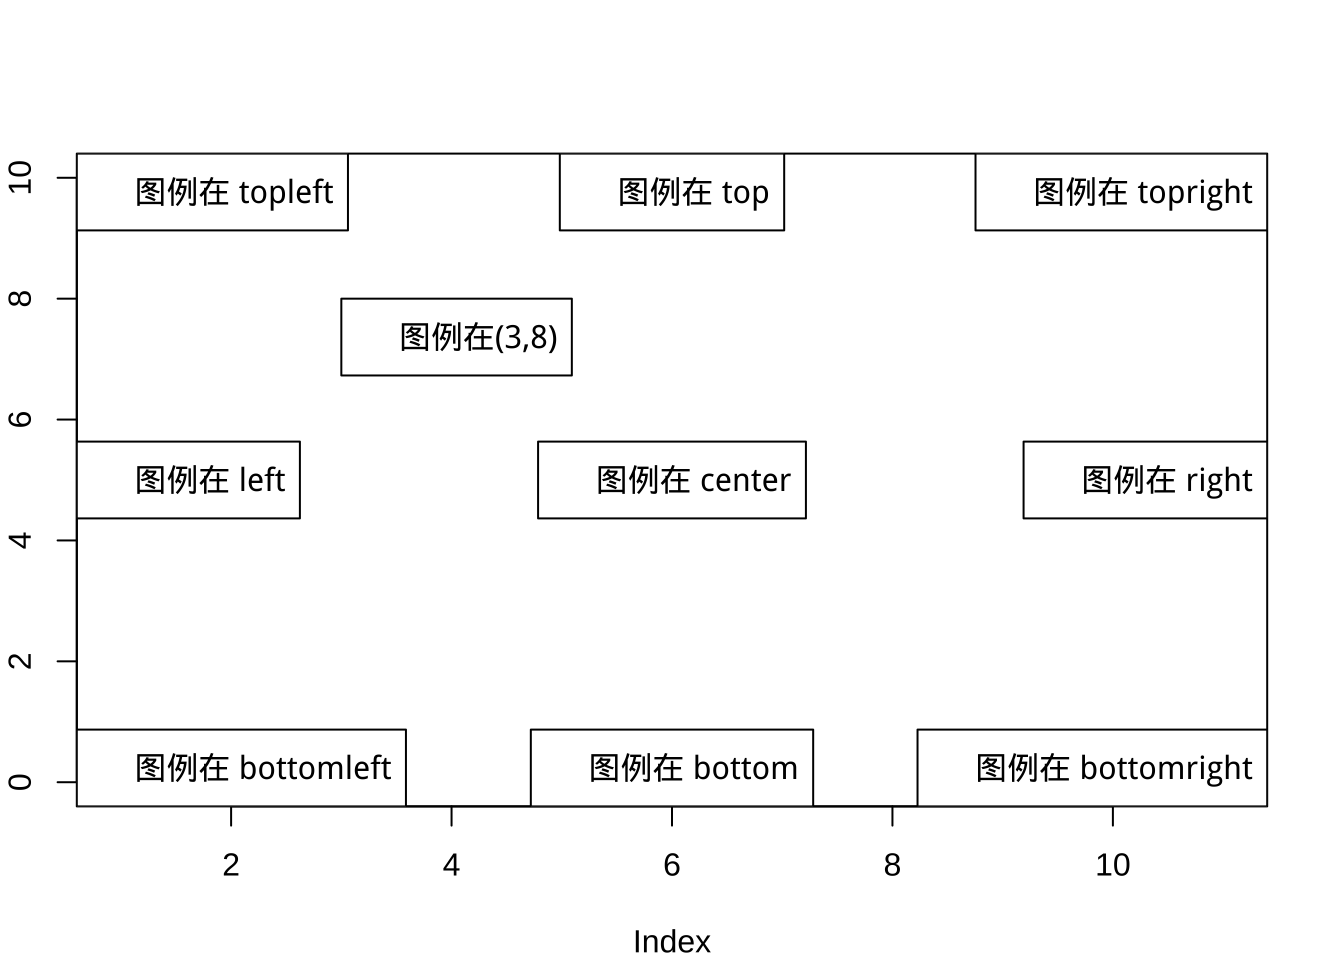
\includegraphics{1001-chapter01_files/figure-latex/unnamed-chunk-33-1} \end{center}

\textbf{综合测试}:

\begin{Shaded}
\begin{Highlighting}[]
\FunctionTok{plot}\NormalTok{(iris}\SpecialCharTok{$}\NormalTok{Sepal.Length, iris}\SpecialCharTok{$}\NormalTok{Sepal.Width, }\AttributeTok{col =}\NormalTok{ iris}\SpecialCharTok{$}\NormalTok{Species, }\AttributeTok{main =} \FunctionTok{list}\NormalTok{(}\StringTok{"鸢尾花的花萼长与宽的散点图"}\NormalTok{, }
    \AttributeTok{cex =} \FloatTok{1.5}\NormalTok{), }\AttributeTok{xlab =} \StringTok{"花萼长度"}\NormalTok{, }\AttributeTok{ylab =} \StringTok{"花萼宽度"}\NormalTok{, }\AttributeTok{pch =} \DecValTok{19}\NormalTok{)}
\FunctionTok{grid}\NormalTok{(}\AttributeTok{nx =} \DecValTok{5}\NormalTok{, }\AttributeTok{ny =} \DecValTok{5}\NormalTok{, }\AttributeTok{lty =} \DecValTok{2}\NormalTok{, }\AttributeTok{col =} \StringTok{"grey"}\NormalTok{)  }\CommentTok{\# 添加网格线}
\FunctionTok{legend}\NormalTok{(}\DecValTok{7}\NormalTok{, }\FloatTok{4.5}\NormalTok{, }\FunctionTok{c}\NormalTok{(}\StringTok{"setosa"}\NormalTok{, }\StringTok{"versicolor"}\NormalTok{, }\StringTok{"virginica"}\NormalTok{), }\AttributeTok{pch =} \DecValTok{19}\NormalTok{, }\AttributeTok{col =} \DecValTok{1}\SpecialCharTok{:}\DecValTok{3}\NormalTok{)  }\CommentTok{\# 添加图例}
\FunctionTok{lines}\NormalTok{(}\FunctionTok{c}\NormalTok{(}\FloatTok{4.3}\NormalTok{, }\FloatTok{6.5}\NormalTok{), }\FunctionTok{c}\NormalTok{(}\DecValTok{2}\NormalTok{, }\FloatTok{4.5}\NormalTok{), }\AttributeTok{col =} \StringTok{"blue"}\NormalTok{)  }\CommentTok{\# 添加直线}
\FunctionTok{arrows}\NormalTok{(}\DecValTok{6}\NormalTok{, }\DecValTok{4}\NormalTok{, }\FloatTok{6.5}\NormalTok{, }\DecValTok{4}\NormalTok{, }\AttributeTok{angle =} \DecValTok{10}\NormalTok{, }\AttributeTok{cex =} \FloatTok{0.5}\NormalTok{)  }\CommentTok{\# 添加箭头}
\FunctionTok{text}\NormalTok{(}\FloatTok{6.9}\NormalTok{, }\DecValTok{4}\NormalTok{, }\StringTok{"左上角全是setosa"}\NormalTok{, }\AttributeTok{cex =} \FloatTok{0.8}\NormalTok{)  }\CommentTok{\# 添加文字说明}
\end{Highlighting}
\end{Shaded}

\begin{center}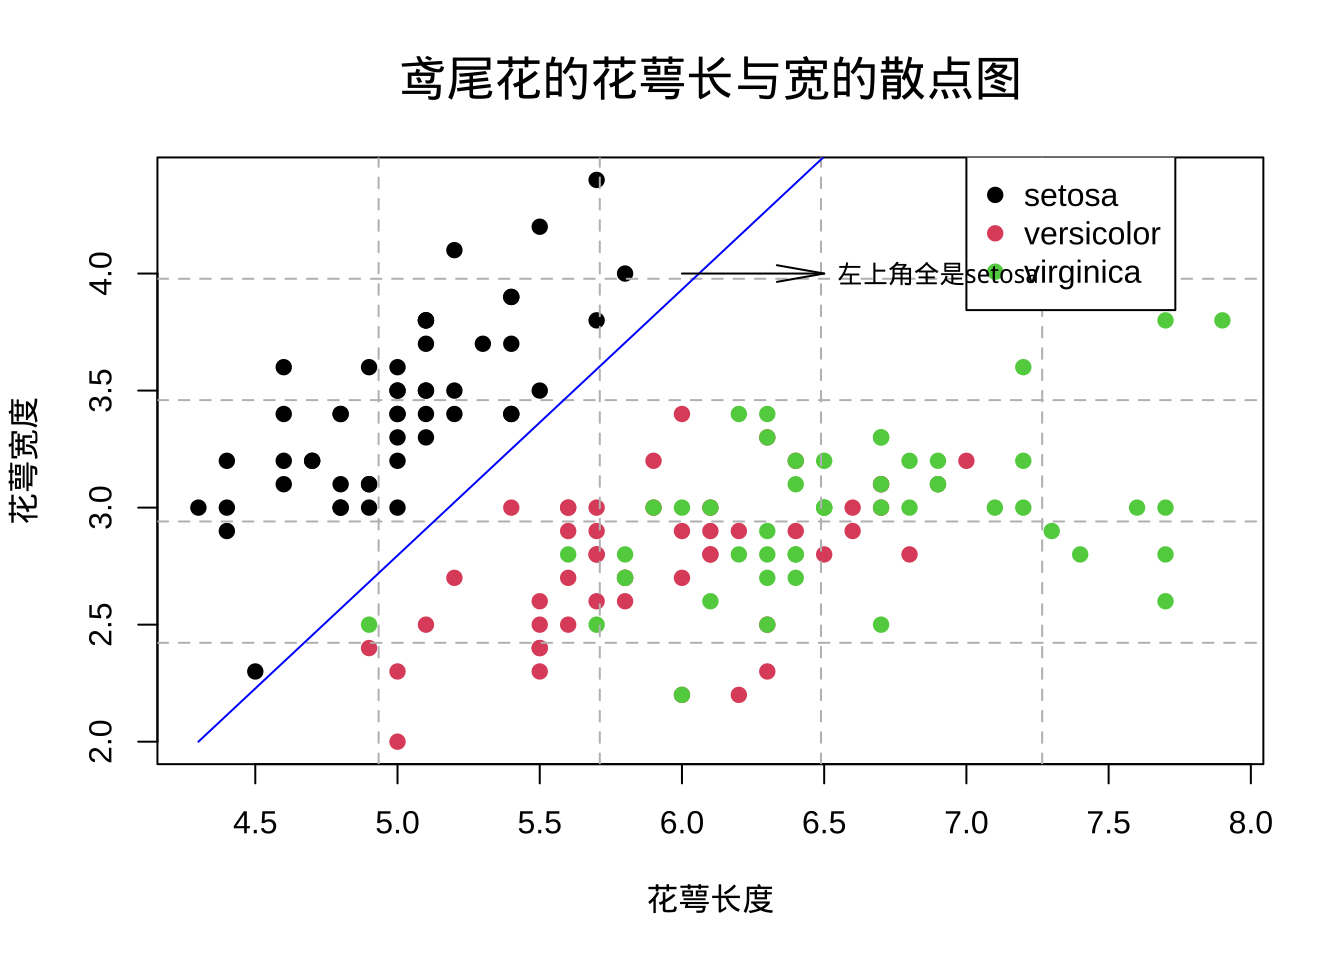
\includegraphics{1001-chapter01_files/figure-latex/unnamed-chunk-34-1} \end{center}

\hypertarget{ux7ed8ux5236ux7ec4ux5408ux56feux5f62}{%
\section{绘制组合图形}\label{ux7ed8ux5236ux7ec4ux5408ux56feux5f62}}

\hypertarget{par}{%
\subsection{par()}\label{par}}

一页多图用mfrow参数或mfcol参数规定。

\begin{Shaded}
\begin{Highlighting}[]
\NormalTok{mfrow1 }\OtherTok{=} \FunctionTok{par}\NormalTok{(}\AttributeTok{mfrow =} \FunctionTok{c}\NormalTok{(}\DecValTok{2}\NormalTok{, }\DecValTok{3}\NormalTok{))  }\CommentTok{\#mar=c(2,2,2,2)}
\ControlFlowTok{for}\NormalTok{ (i }\ControlFlowTok{in} \DecValTok{1}\SpecialCharTok{:}\DecValTok{6}\NormalTok{) \{}
    \FunctionTok{plot}\NormalTok{(}\FunctionTok{c}\NormalTok{(}\DecValTok{1}\SpecialCharTok{:}\NormalTok{i), }\AttributeTok{main =} \FunctionTok{paste}\NormalTok{(}\StringTok{"I\textquotesingle{}m image:"}\NormalTok{, i))}
\NormalTok{\}}
\end{Highlighting}
\end{Shaded}

\begin{center}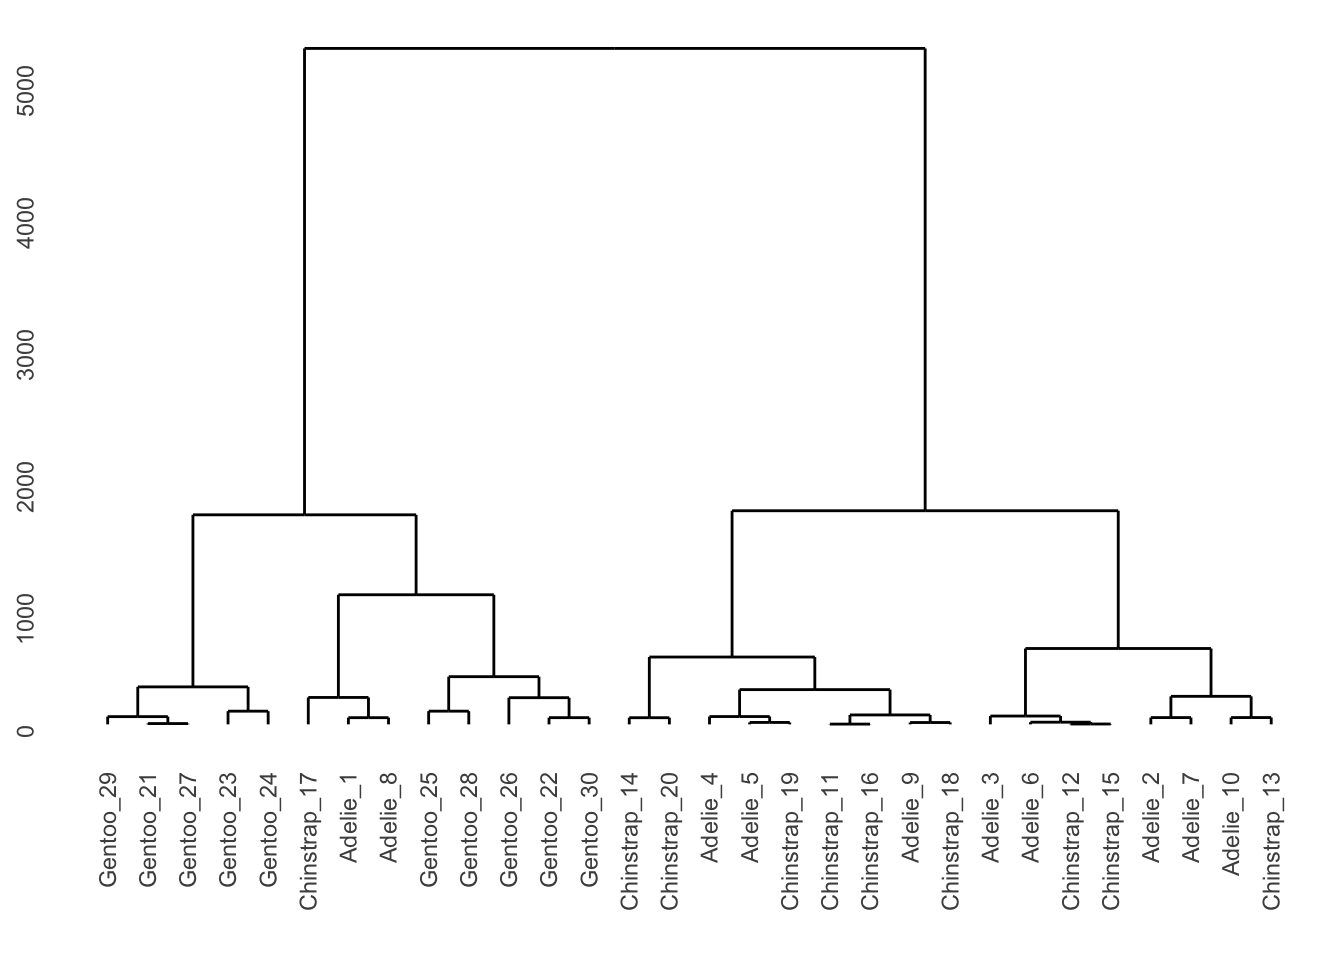
\includegraphics{1001-chapter01_files/figure-latex/unnamed-chunk-35-1} \end{center}

\begin{Shaded}
\begin{Highlighting}[]
\FunctionTok{par}\NormalTok{(mfrow1)}

\NormalTok{op }\OtherTok{=} \FunctionTok{par}\NormalTok{(}\AttributeTok{mfrow =} \FunctionTok{c}\NormalTok{(}\DecValTok{2}\NormalTok{, }\DecValTok{2}\NormalTok{))}
\FunctionTok{plot}\NormalTok{(}\DecValTok{1}\SpecialCharTok{:}\DecValTok{10}\NormalTok{, }\AttributeTok{pch =} \DecValTok{12}\NormalTok{)}
\FunctionTok{hist}\NormalTok{(}\DecValTok{1}\SpecialCharTok{:}\DecValTok{10}\NormalTok{)}
\FunctionTok{boxplot}\NormalTok{(}\DecValTok{1}\SpecialCharTok{:}\DecValTok{10}\NormalTok{)}
\FunctionTok{pie}\NormalTok{(}\DecValTok{1}\SpecialCharTok{:}\DecValTok{10}\NormalTok{)}
\end{Highlighting}
\end{Shaded}

\begin{center}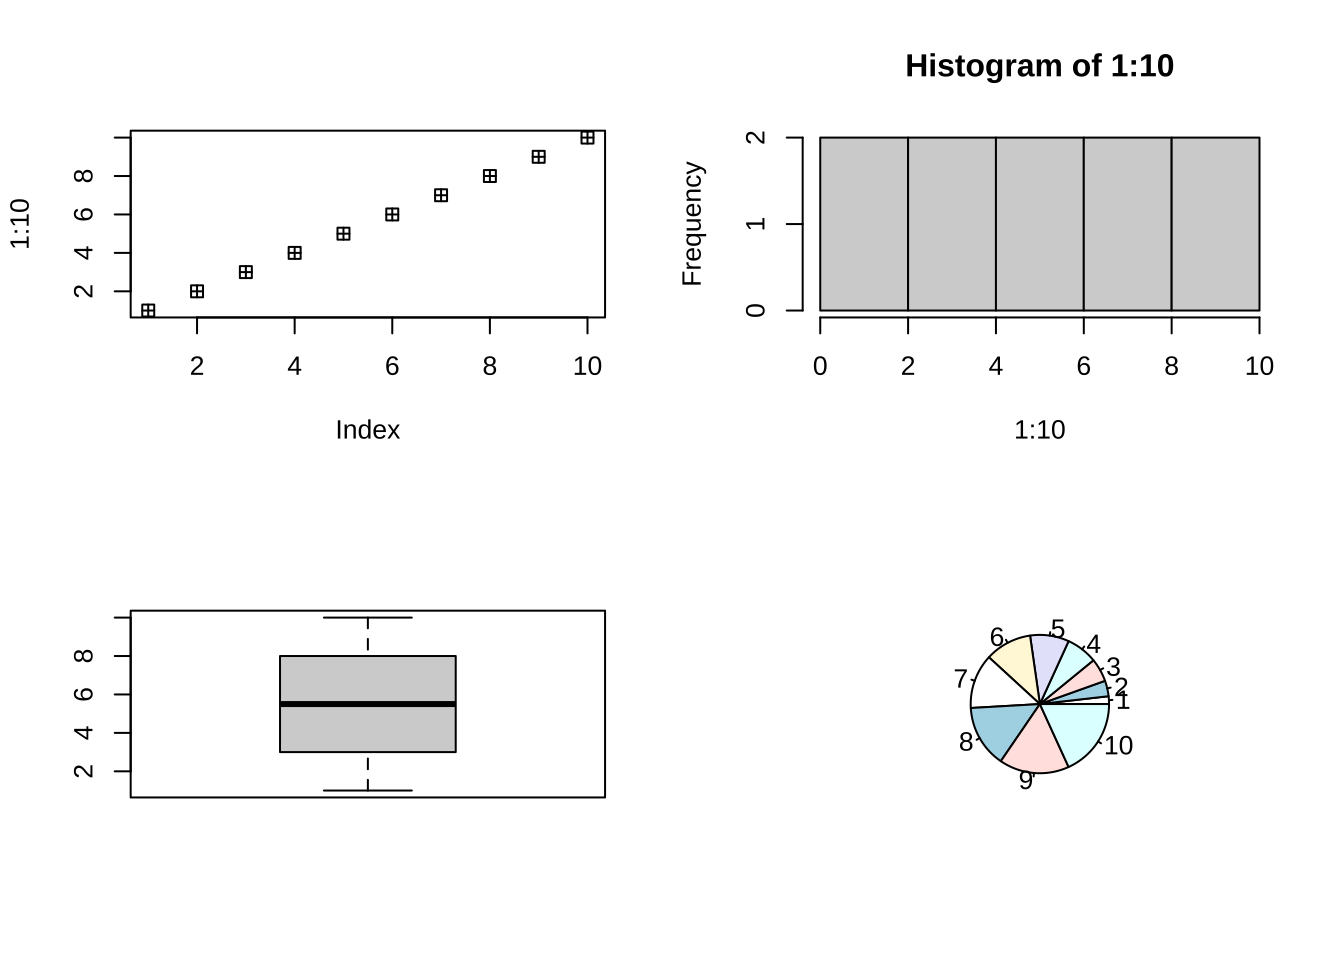
\includegraphics{1001-chapter01_files/figure-latex/unnamed-chunk-35-2} \end{center}

\begin{Shaded}
\begin{Highlighting}[]
\FunctionTok{par}\NormalTok{(op)}
\end{Highlighting}
\end{Shaded}

\hypertarget{layout}{%
\subsection{layout}\label{layout}}

与par函数均分画布不同,layout函数可以不均等的分隔页面

\begin{Shaded}
\begin{Highlighting}[]
\NormalTok{mat }\OtherTok{\textless{}{-}} \FunctionTok{matrix}\NormalTok{(}\FunctionTok{c}\NormalTok{(}\DecValTok{1}\NormalTok{, }\DecValTok{1}\NormalTok{, }\DecValTok{1}\NormalTok{, }\DecValTok{2}\NormalTok{, }\DecValTok{3}\NormalTok{, }\DecValTok{3}\NormalTok{, }\DecValTok{4}\NormalTok{, }\DecValTok{4}\NormalTok{, }\DecValTok{5}\NormalTok{, }\DecValTok{5}\NormalTok{, }\DecValTok{5}\NormalTok{, }\DecValTok{6}\NormalTok{), }\AttributeTok{nrow =} \DecValTok{2}\NormalTok{, }\AttributeTok{byrow =} \ConstantTok{TRUE}\NormalTok{)}
\FunctionTok{layout}\NormalTok{(mat)}
\ControlFlowTok{for}\NormalTok{ (i }\ControlFlowTok{in} \DecValTok{1}\SpecialCharTok{:}\DecValTok{6}\NormalTok{) \{}
    \FunctionTok{plot}\NormalTok{(}\FunctionTok{c}\NormalTok{(}\DecValTok{1}\SpecialCharTok{:}\NormalTok{i), }\AttributeTok{main =} \FunctionTok{paste}\NormalTok{(}\StringTok{"I\textquotesingle{}m image:"}\NormalTok{, i))}
\NormalTok{\}}
\end{Highlighting}
\end{Shaded}

\begin{center}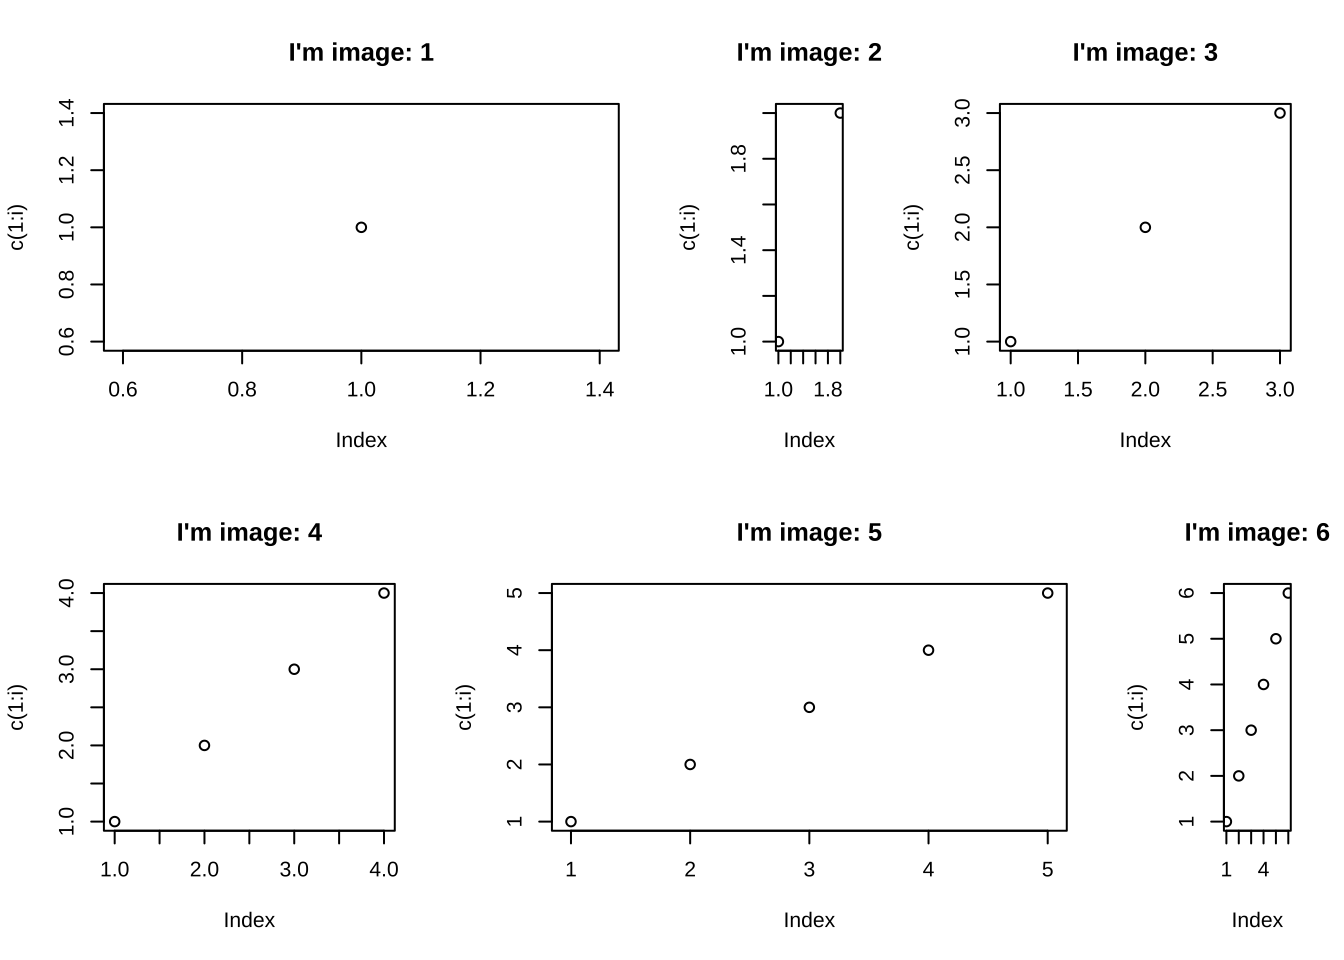
\includegraphics{1001-chapter01_files/figure-latex/unnamed-chunk-36-1} \end{center}

\hypertarget{ux4fddux5b58ux56feux5f62}{%
\section{保存图形}\label{ux4fddux5b58ux56feux5f62}}

\hypertarget{ux4f7fux7528ux4ee3ux7801}{%
\subsection{使用代码}\label{ux4f7fux7528ux4ee3ux7801}}

对于其他格式输出类似pdf的输出。

\begin{Shaded}
\begin{Highlighting}[]
\FunctionTok{pdf}\NormalTok{(}\StringTok{"test/2.pdf"}\NormalTok{)  }\CommentTok{\# 保存到当前工作目录下}
\FunctionTok{plot}\NormalTok{(}\DecValTok{1}\SpecialCharTok{:}\DecValTok{10}\NormalTok{)}
\FunctionTok{dev.off}\NormalTok{()}
\end{Highlighting}
\end{Shaded}

\begin{verbatim}
## pdf 
##   2
\end{verbatim}

\hypertarget{ux5728-rstudio-ux7a97ux53e3ux70b9ux51fbux6309ux94aeux4fddux5b58}{%
\subsection{在 Rstudio 窗口点击按钮保存}\label{ux5728-rstudio-ux7a97ux53e3ux70b9ux51fbux6309ux94aeux4fddux5b58}}

\begin{figure}
\centering
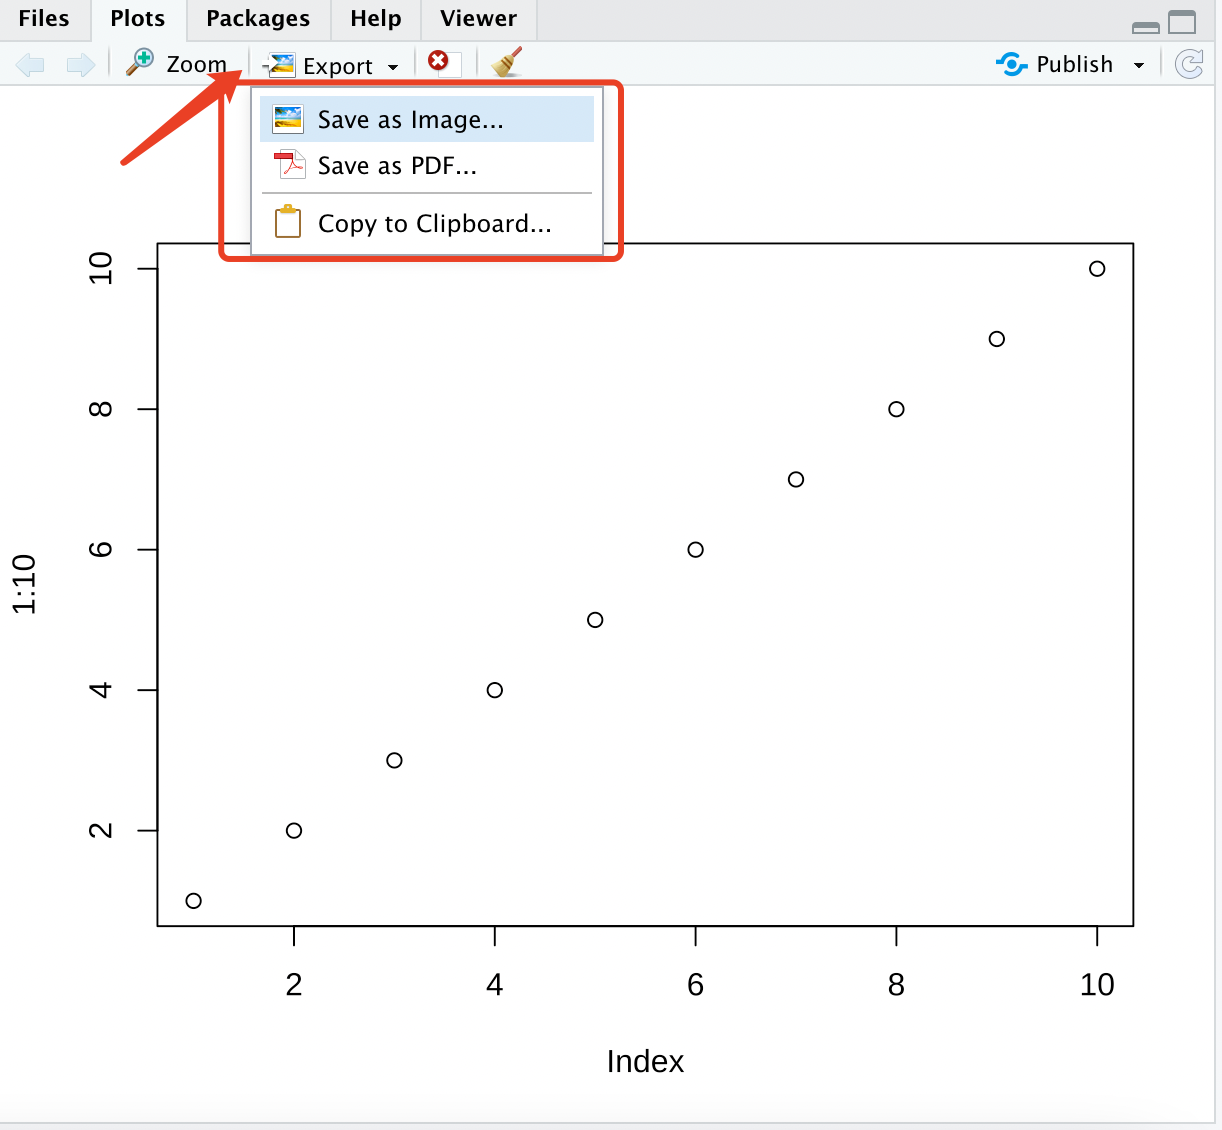
\includegraphics{figure/12.png}
\caption{Rstudio界面右下角}
\end{figure}

\begin{figure}
\centering
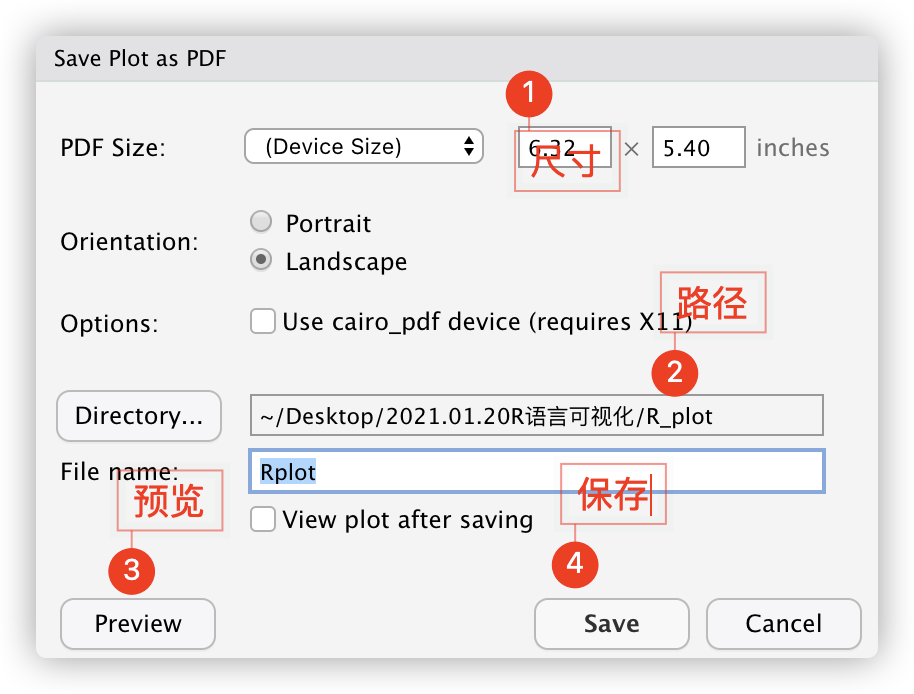
\includegraphics{figure/13.png}
\caption{自定义设置}
\end{figure}

\hypertarget{ggplot2-plot}{%
\chapter{使用 ggplot2 包绘图}\label{ggplot2-plot}}

\hypertarget{ux7b80ux4ecb-1}{%
\section{简介}\label{ux7b80ux4ecb-1}}

ggplot2 包是 Harley
Wickham 在 2005 年创建的,是包含了一套全面而连贯的语法的绘图系统。

\begin{figure}
\centering

\includegraphics{figure/15.png}
\caption{Harley Wickham}
\end{figure}

弥补了R中创建图形缺乏一致性的缺点,且不会局限于一些已经定义好的统计图形,可以根据需要创造出任何有助于解决所遇到问题的图形。

\textbf{核心理念}:将绘图与数据分离,数据相关的绘图与数据无关的绘图分离,\textbf{按图层作图}。

\hypertarget{qplot}{%
\section{qplot}\label{qplot}}

\texttt{ggplot2}包的绘图语言与常用的绘图函数的使用方法不同,为了让读者快速使用\texttt{ggplot2}包,包的作者Harley
Wickham提供了\texttt{qplot}函数(quick
plot),让人在了解\texttt{ggplot2}的语言逻辑之前,就能迅速实现数据的可视化。

鸢尾花数据集\texttt{iris}

\begin{Shaded}
\begin{Highlighting}[]
\FunctionTok{head}\NormalTok{(iris, }\DecValTok{10}\NormalTok{)}
\end{Highlighting}
\end{Shaded}

\begin{verbatim}
##    Sepal.Length Sepal.Width Petal.Length Petal.Width Species
## 1           5.1         3.5          1.4         0.2  setosa
## 2           4.9         3.0          1.4         0.2  setosa
## 3           4.7         3.2          1.3         0.2  setosa
## 4           4.6         3.1          1.5         0.2  setosa
## 5           5.0         3.6          1.4         0.2  setosa
## 6           5.4         3.9          1.7         0.4  setosa
## 7           4.6         3.4          1.4         0.3  setosa
## 8           5.0         3.4          1.5         0.2  setosa
## 9           4.4         2.9          1.4         0.2  setosa
## 10          4.9         3.1          1.5         0.1  setosa
\end{verbatim}

\begin{Shaded}
\begin{Highlighting}[]
\FunctionTok{str}\NormalTok{(iris)}
\end{Highlighting}
\end{Shaded}

\begin{verbatim}
## 'data.frame':    150 obs. of  5 variables:
##  $ Sepal.Length: num  5.1 4.9 4.7 4.6 5 5.4 4.6 5 4.4 4.9 ...
##  $ Sepal.Width : num  3.5 3 3.2 3.1 3.6 3.9 3.4 3.4 2.9 3.1 ...
##  $ Petal.Length: num  1.4 1.4 1.3 1.5 1.4 1.7 1.4 1.5 1.4 1.5 ...
##  $ Petal.Width : num  0.2 0.2 0.2 0.2 0.2 0.4 0.3 0.2 0.2 0.1 ...
##  $ Species     : Factor w/ 3 levels "setosa","versicolor",..: 1 1 1 1 1 1 1 1 1 1 ...
\end{verbatim}

\begin{itemize}
\tightlist
\item
  \textbf{例子一:}
\end{itemize}

创建一个以物种种类为分组的花萼长度的箱线图,箱线图的颜色依据不同的物种种类而变化。

\begin{Shaded}
\begin{Highlighting}[]
\FunctionTok{library}\NormalTok{(ggplot2)}
\FunctionTok{qplot}\NormalTok{(Species, Sepal.Length, }\AttributeTok{data =}\NormalTok{ iris, }\AttributeTok{geom =} \StringTok{"boxplot"}\NormalTok{, }\AttributeTok{fill =}\NormalTok{ Species, }\AttributeTok{main =} \StringTok{"依据种类分组的花萼长度箱线图"}\NormalTok{)}
\end{Highlighting}
\end{Shaded}

\begin{center}\includegraphics{2001-chapter02_files/figure-latex/unnamed-chunk-3-1} \end{center}

\begin{Shaded}
\begin{Highlighting}[]
\FunctionTok{boxplot}\NormalTok{(Sepal.Length }\SpecialCharTok{\textasciitilde{}}\NormalTok{ Species, }\AttributeTok{data =}\NormalTok{ iris, }\AttributeTok{main =} \StringTok{"依据种类分组的花萼长度箱线图"}\NormalTok{)}
\end{Highlighting}
\end{Shaded}

\begin{center}\includegraphics{2001-chapter02_files/figure-latex/unnamed-chunk-3-2} \end{center}

\begin{itemize}
\tightlist
\item
  \textbf{例子二:}
\end{itemize}

利用\texttt{qplot}函数画出小提琴图,只需要将\texttt{geom}设置为\texttt{“violon”}即可,并添加扰动以减少数据重叠。

\begin{Shaded}
\begin{Highlighting}[]
\FunctionTok{qplot}\NormalTok{(Species, Sepal.Length, }\AttributeTok{data =}\NormalTok{ iris, }\AttributeTok{geom =} \FunctionTok{c}\NormalTok{(}\StringTok{"violin"}\NormalTok{, }\StringTok{"jitter"}\NormalTok{), }\AttributeTok{fill =}\NormalTok{ Species, }
    \AttributeTok{main =} \StringTok{"依据种类分组的花萼长度小提琴图"}\NormalTok{)}
\end{Highlighting}
\end{Shaded}

\begin{center}\includegraphics{2001-chapter02_files/figure-latex/unnamed-chunk-4-1} \end{center}

\begin{itemize}
\tightlist
\item
  \textbf{例子三:}
\end{itemize}

建一个以花萼长度和花萼宽度的散点图,并利用颜色和符号形状区分物种种类。

\begin{Shaded}
\begin{Highlighting}[]
\FunctionTok{qplot}\NormalTok{(Sepal.Length, Sepal.Width, }\AttributeTok{geom =} \StringTok{"point"}\NormalTok{, }\AttributeTok{data =}\NormalTok{ iris, }\AttributeTok{colour =}\NormalTok{ Species, }\AttributeTok{shape =}\NormalTok{ Species, }
    \AttributeTok{main =} \StringTok{"绘制花萼长度和花萼宽度的散点图"}\NormalTok{)}
\end{Highlighting}
\end{Shaded}

\begin{center}\includegraphics{2001-chapter02_files/figure-latex/unnamed-chunk-5-1} \end{center}

\begin{itemize}
\tightlist
\item
  \textbf{例子四:}
\end{itemize}

利用facets参数绘制分面板散点图,并增加光滑曲线。

\begin{Shaded}
\begin{Highlighting}[]
\FunctionTok{qplot}\NormalTok{(Sepal.Length, Sepal.Width, }\AttributeTok{data =}\NormalTok{ iris, }\AttributeTok{geom =} \FunctionTok{c}\NormalTok{(}\StringTok{"point"}\NormalTok{, }\StringTok{"smooth"}\NormalTok{), }\AttributeTok{facets =} \SpecialCharTok{\textasciitilde{}}\NormalTok{Species, }
    \AttributeTok{main =} \StringTok{"绘制分面板的散点图"}\NormalTok{)}
\end{Highlighting}
\end{Shaded}

\begin{center}\includegraphics{2001-chapter02_files/figure-latex/unnamed-chunk-6-1} \end{center}

\hypertarget{ggplot2ux5305ux56feux5f62ux8bedux6cd5}{%
\section{ggplot2包图形语法}\label{ggplot2ux5305ux56feux5f62ux8bedux6cd5}}

\textbf{推荐书籍}:

ggplot2: Elegant Graphics for Data Analysis \url{https://ggplot2-book.org/}

Fundamentals of Data Visualization \url{https://clauswilke.com/dataviz/}

\hypertarget{ux5bf9ux6bd4ux4e0dux540cux753bux56feux8bedux6cd5}{%
\subsection{对比不同画图语法}\label{ux5bf9ux6bd4ux4e0dux540cux753bux56feux8bedux6cd5}}

以绘制iris数据集中Sepal.Length与Sepal.Width的散点图为例,分别采用内置的plot函数与ggplot2包的ggplot函数绘制散点图,对比理解ggplot2包的语言逻辑。

代码(三种类型):

\begin{Shaded}
\begin{Highlighting}[]
\CommentTok{\# 基础包}
\FunctionTok{plot}\NormalTok{(iris}\SpecialCharTok{$}\NormalTok{Sepal.Length, iris}\SpecialCharTok{$}\NormalTok{Sepal.Width)}
\end{Highlighting}
\end{Shaded}

\begin{center}\includegraphics{2001-chapter02_files/figure-latex/unnamed-chunk-8-1} \end{center}

\begin{Shaded}
\begin{Highlighting}[]
\CommentTok{\# qplot()}
\FunctionTok{qplot}\NormalTok{(}\AttributeTok{x =}\NormalTok{ Sepal.Length, }\AttributeTok{y =}\NormalTok{ Sepal.Width,}\AttributeTok{data =}\NormalTok{ iris,}\AttributeTok{geom =} \StringTok{"point"}\NormalTok{)}
\end{Highlighting}
\end{Shaded}

\begin{center}\includegraphics{2001-chapter02_files/figure-latex/unnamed-chunk-8-2} \end{center}

\begin{Shaded}
\begin{Highlighting}[]
\CommentTok{\# ggplot()}
\FunctionTok{ggplot}\NormalTok{(}\AttributeTok{data=}\NormalTok{ iris, }\FunctionTok{aes}\NormalTok{(}\AttributeTok{x =}\NormalTok{ Sepal.Length, }\AttributeTok{y =}\NormalTok{ Sepal.Width)) }\SpecialCharTok{+}  \CommentTok{\#绘制底层画布}
\FunctionTok{geom\_point}\NormalTok{()  }\CommentTok{\#在画布上添加点}
\end{Highlighting}
\end{Shaded}

\begin{center}\includegraphics{2001-chapter02_files/figure-latex/unnamed-chunk-8-3} \end{center}

\hypertarget{ux601dux60f3ux4ecbux7ecd}{%
\subsection{思想介绍}\label{ux601dux60f3ux4ecbux7ecd}}

\textbf{注:}该部分主要参考\href{https://bookdown.org/wangminjie/R4DS/intro-R.html\#\%E5\%AE\%89\%E8\%A3\%85-rstudio}{数据科学中的R语言------王敏杰}。

ggplot的绘图有以下几个特点。

\begin{enumerate}
\def\labelenumi{\arabic{enumi}.}
\item
  有明确的起始(以ggplot函数开始)与终止(一句语句一幅图)。
\item
  ggplot2语句可以理解为一句语句绘制一幅图,然后进行图层叠加,而叠加是通过''+``号把绘图语句拼接实现的。
\end{enumerate}

ggplot函数包括9个部件:

\begin{itemize}
\tightlist
\item
  数据 (data) ( 数据框)
\item
  映射 (mapping)
\item
  几何对象 (geom\_point() , geom\_boxplot())
\item
  统计变换 (stats)
\item
  标度 (scale)
\item
  坐标系 (coord)
\item
  分面 (facet)
\item
  主题 (theme)
\item
  存储和输出 (output)
\end{itemize}

其中前三个是必需的。

Hadley
Wickham将这套可视化语法诠释为:一张统计图形就是从\textbf{数据}到\textbf{几何对象}(geometric
object,缩写geom)的\textbf{图形属性}(aesthetic
attribute,缩写aes)的一个映射。

\includegraphics{figure/10.png}

此外,图形中还可能包含数据的\textbf{统计变换}(statistical
transformation,缩写stats),最后绘制在某个特定的\textbf{坐标系}(coordinate
system,缩写coord)中,而\textbf{分面}(facet)则可以用来生成数据不同子集的图形。

\begin{figure}
\centering
\includegraphics{figure/11.png}
\caption{语法模板}
\end{figure}

\begin{figure}
\centering
\includegraphics{figure/22.png}
\caption{把这看懂其实差不多了}
\end{figure}

\textbf{例子(带你入门)}

\begin{Shaded}
\begin{Highlighting}[]
\FunctionTok{ggplot}\NormalTok{(}\AttributeTok{data =}\NormalTok{ iris, }\AttributeTok{mapping =} \FunctionTok{aes}\NormalTok{(Petal.Length, Petal.Width)) }\SpecialCharTok{+} \FunctionTok{geom\_point}\NormalTok{(}\AttributeTok{size =} \DecValTok{2}\NormalTok{, }
    \AttributeTok{alpha =} \FloatTok{0.5}\NormalTok{, }\AttributeTok{col =} \StringTok{"red"}\NormalTok{) }\SpecialCharTok{+} \FunctionTok{geom\_smooth}\NormalTok{(}\AttributeTok{method =} \StringTok{"lm"}\NormalTok{, }\AttributeTok{se =}\NormalTok{ F)}
\end{Highlighting}
\end{Shaded}

\begin{center}\includegraphics{2001-chapter02_files/figure-latex/unnamed-chunk-9-1} \end{center}

\hypertarget{ux5168ux5c40ux53d8ux91cf-vs.-ux5c40ux90e8ux53d8ux91cf}{%
\subsection{全局变量 vs.~局部变量}\label{ux5168ux5c40ux53d8ux91cf-vs.-ux5c40ux90e8ux53d8ux91cf}}

\begin{Shaded}
\begin{Highlighting}[]
\FunctionTok{ggplot}\NormalTok{(}\AttributeTok{data =}\NormalTok{ iris, }\AttributeTok{mapping =} \FunctionTok{aes}\NormalTok{(}\AttributeTok{x =}\NormalTok{ Petal.Length, }\AttributeTok{y =}\NormalTok{ Petal.Width, }\AttributeTok{col =}\NormalTok{ Species)) }\SpecialCharTok{+} 
    \FunctionTok{geom\_point}\NormalTok{()}
\end{Highlighting}
\end{Shaded}

\begin{center}\includegraphics{2001-chapter02_files/figure-latex/unnamed-chunk-10-1} \end{center}

\begin{Shaded}
\begin{Highlighting}[]
\FunctionTok{ggplot}\NormalTok{(}\AttributeTok{data =}\NormalTok{ iris) }\SpecialCharTok{+} \FunctionTok{geom\_point}\NormalTok{(}\AttributeTok{mapping =} \FunctionTok{aes}\NormalTok{(}\AttributeTok{x =}\NormalTok{ Petal.Length, }\AttributeTok{y =}\NormalTok{ Petal.Width, }
    \AttributeTok{col =}\NormalTok{ Species))}
\end{Highlighting}
\end{Shaded}

\begin{center}\includegraphics{2001-chapter02_files/figure-latex/unnamed-chunk-10-2} \end{center}

大家可以看到,以上两段代码出来的图是一样。但背后的含义却不同。

\textbf{例子(观察两者之间的区别)}

\begin{Shaded}
\begin{Highlighting}[]
\CommentTok{\# 版本一}
\FunctionTok{ggplot}\NormalTok{(}\AttributeTok{data =}\NormalTok{ iris, }\AttributeTok{mapping =} \FunctionTok{aes}\NormalTok{(}\AttributeTok{x =}\NormalTok{ Petal.Length, }\AttributeTok{y =}\NormalTok{ Petal.Width, }\AttributeTok{col =}\NormalTok{ Species)) }\SpecialCharTok{+} 
    \FunctionTok{geom\_point}\NormalTok{() }\SpecialCharTok{+} \FunctionTok{geom\_smooth}\NormalTok{()}
\end{Highlighting}
\end{Shaded}

\begin{center}\includegraphics{2001-chapter02_files/figure-latex/unnamed-chunk-11-1} \end{center}

\begin{Shaded}
\begin{Highlighting}[]
\CommentTok{\# 版本二}
\FunctionTok{ggplot}\NormalTok{(}\AttributeTok{data =}\NormalTok{ iris, }\AttributeTok{mapping =} \FunctionTok{aes}\NormalTok{(}\AttributeTok{x =}\NormalTok{ Petal.Length, }\AttributeTok{y =}\NormalTok{ Petal.Width)) }\SpecialCharTok{+} \FunctionTok{geom\_point}\NormalTok{(}\AttributeTok{mapping =} \FunctionTok{aes}\NormalTok{(}\AttributeTok{col =}\NormalTok{ Species)) }\SpecialCharTok{+} 
    \FunctionTok{geom\_smooth}\NormalTok{()}
\end{Highlighting}
\end{Shaded}

\begin{center}\includegraphics{2001-chapter02_files/figure-latex/unnamed-chunk-11-2} \end{center}

\hypertarget{ux51e0ux4f55ux5bf9ux8c61}{%
\section{几何对象}\label{ux51e0ux4f55ux5bf9ux8c61}}

\texttt{geom\_xxx()}提供了各种基本图形。 列表如下:

\begin{itemize}
\item
  基础图形:

  \begin{itemize}
  \tightlist
  \item
    \texttt{geom\_blank()}不画图,可以按映射的变量设定坐标范围;
  \item
    \texttt{geom\_point()}每个观测为一个散点;
  \item
    \texttt{geom\_hline()}, \texttt{geom\_vline()}, \texttt{geom\_abline()}画线;
  \item
    \texttt{geom\_path()}每个观测提供坐标,在相邻观测之间连线;
  \item
    \texttt{geom\_ribbon()}需要x和ymin,
    ymax维,在从小到大排序后的相邻观测之间连接阴影区域;
  \item
    \texttt{geom\_segment()}需要x, y和xend, yend,为每个观测画一条线段;
  \item
    \texttt{geom\_rect()}需要xmin, xmax, ymin,
    ymax,为每个观测画一个长方形,可有填充色;
  \item
    \texttt{geom\_polygon()}需要x,
    y,将相邻观测连续并连接成一个闭合的多边形,中间填充颜色;
  \item
    \texttt{geom\_text()}需要x, y和lable,每个观测画一条文字标签。
  \end{itemize}
\item
  单变量图层:

  \begin{itemize}
  \tightlist
  \item
    \texttt{geom\_bar()}, \texttt{geom\_col()}作条形图;
  \item
    \texttt{geom\_histogram()}对连续变量x作直方图;
  \item
    \texttt{geom\_density()}对连续变量x作一元密度估计曲线;
  \item
    \texttt{geom\_dotplot()}用原点作直方图;
  \item
    \texttt{geom\_freqpoly()}用折线作直方图。
  \end{itemize}
\item
  两变量图形:

  \begin{itemize}
  \item
    两个连续变量x, y:

    \begin{itemize}
    \tightlist
    \item
      \texttt{geom\_point()}散点图;
    \item
      \texttt{geom\_quantile()}拟合分位数回归曲线;
    \item
      \texttt{geom\_rug()}在坐标轴处画数值对应的短须线;
    \item
      \texttt{geom\_smooth()}画各种拟合曲线;
    \item
      \texttt{geom\_text()}在指定的x, y位置画label给出的文字标签;
    \end{itemize}
  \item
    显示二元分布:

    \begin{itemize}
    \tightlist
    \item
      \texttt{geom\_bin2d()}作长方形分块的二维直方图;
    \item
      \texttt{geom\_density2d()}作二元密度估计等值线图;
    \item
      \texttt{geom\_hex()}作正六边形分块的二维直方图。
    \end{itemize}
  \item
    两个变量中有分类变量时:

    \begin{itemize}
    \tightlist
    \item
      \texttt{geom\_count()}:重叠点越多画点越大;
    \item
      \texttt{geom\_jitter()}:
      随机扰动散点位置避免重叠,数值变量有重叠时也可以用;
    \end{itemize}
  \item
    一个连续变量和一个分类变量:

    \begin{itemize}
    \tightlist
    \item
      \texttt{geom\_col()}作条形图,对分类变量的每个值画一个条形,长度与连续变量值成比例;
    \item
      \texttt{geom\_boxplot()}对每个类做一个盒形图;
    \item
      \texttt{geom\_violin()}对每个类做一个小提琴图。
    \end{itemize}
  \item
    一个时间变量和一个连续变量:

    \begin{itemize}
    \tightlist
    \item
      \texttt{geom\_area()}作阴影曲线图,曲线下方填充阴影色;
    \item
      \texttt{geom\_line()}作折线图,在相邻两个时间之间连接线段;
    \item
      \texttt{geom\_step()}作阶梯函数图,在相邻两个时间之间连接阶梯函数线。
    \end{itemize}
  \item
    不确定性:

    \begin{itemize}
    \tightlist
    \item
      \texttt{geom\_crossbar()}对每个观测输入的x, y, ymin,
      ymax画中间有线的纵向条形;
    \item
      \texttt{geom\_errbar()}对每个观测输入的x, ymin, ymax画纵向误差条;
    \item
      \texttt{geom\_linerange()}对每个观测输入的x, ymin, ymax画一条竖线;
    \item
      \texttt{geom\_pointrnage()}对每个观测输入的x, y, ymin,
      ymax画一条中间有点的竖线。
    \end{itemize}
  \end{itemize}
\item
  地图:

  \begin{itemize}
  \tightlist
  \item
    \texttt{geom\_map()}: 用区域边界坐标数据画边界线地图。
  \end{itemize}
\item
  三个变量:

  \begin{itemize}
  \item
    \texttt{geom\_contour()}: 用输入的x, y, z数据画等值线图。
  \item
    \texttt{geom\_tile()}用输入的x, y位置, width,
    height大小和指定的fill维画长方形色块填充图。
  \item
    \texttt{geom\_raster()}是\texttt{geom\_tile()}的长方形大小相同时的快速版本。
  \end{itemize}
\end{itemize}

\hypertarget{ux53c2ux8003ux4e66ux7c4d}{%
\subsection{参考书籍}\label{ux53c2ux8003ux4e66ux7c4d}}

由于这部分内容非常的多,短短两小时不可能讲完,这里给了一些参考资料,各个都是满满的干货。

\begin{itemize}
\item
  \href{https://bookdown.org/wangminjie/R4DS/ggplot2-geom.html\#\%E5\%9F\%BA\%E6\%9C\%AC\%E7\%BB\%98\%E5\%9B\%BE}{数据科学中的R-第14章ggplot之集合对象}
\item
  \href{https://www.math.pku.edu.cn/teachers/lidf/docs/Rbook/html/_Rbook/ggplotvis.html}{R语言教程第30节-ggplot各种图形}
\item
  \href{http://r-statistics.co/Top50-Ggplot2-Visualizations-MasterList-R-Code.html}{Top 50 ggplot2
  Visualizations}
\item
  \href{http://r4ds.had.co.nz/data-visualisation.html}{Chapter 3: Data
  Visualisation} of \emph{R
  for Data Science}
\item
  \href{http://r4ds.had.co.nz/graphics-for-communication.html}{Chapter 28: Graphics for
  communication}
  of \emph{R for Data Science}
\item
  \href{https://r-graphics.org/}{Graphs} in \emph{R Graphics Cookbook}
\end{itemize}

\hypertarget{ux7edfux8ba1ux53d8ux6362}{%
\section{统计变换}\label{ux7edfux8ba1ux53d8ux6362}}

\textbf{概念}:对数据所应用的统计类型/方法。

ggplot2为每一种几何类型指定了一种默认的统计类型,如果仅指定geom或stat中的一个,另外一个会自动获取。其中,stat\_identity则表示不做任何的统计变换。

\textbf{示例}:只需指定geom或stat中的一个,具体细小细节可以参考这
\url{https://bookdown.org/wangminjie/R4DS/ggplot2-stat-layer.html}

\begin{Shaded}
\begin{Highlighting}[]
\FunctionTok{ggplot}\NormalTok{(iris) }\SpecialCharTok{+} \FunctionTok{geom\_bar}\NormalTok{(}\FunctionTok{aes}\NormalTok{(}\AttributeTok{x =}\NormalTok{ Sepal.Length), }\AttributeTok{stat =} \StringTok{"bin"}\NormalTok{, }\AttributeTok{binwidth =} \FloatTok{0.5}\NormalTok{)}
\end{Highlighting}
\end{Shaded}

\begin{center}\includegraphics{2001-chapter02_files/figure-latex/unnamed-chunk-12-1} \end{center}

\begin{Shaded}
\begin{Highlighting}[]
\FunctionTok{ggplot}\NormalTok{(iris) }\SpecialCharTok{+} \FunctionTok{stat\_bin}\NormalTok{(}\FunctionTok{aes}\NormalTok{(}\AttributeTok{x =}\NormalTok{ Sepal.Length), }\AttributeTok{geom =} \StringTok{"bar"}\NormalTok{, }\AttributeTok{binwidth =} \FloatTok{0.5}\NormalTok{)}
\end{Highlighting}
\end{Shaded}

\begin{center}\includegraphics{2001-chapter02_files/figure-latex/unnamed-chunk-12-2} \end{center}

\hypertarget{ux523bux5ea6scale}{%
\section{刻度scale}\label{ux523bux5ea6scale}}

这一节我们一起学习ggplot2中的scales语法,推荐大家阅读Hadley
Wickham最新版的\href{https://ggplot2-book.org/}{《ggplot2: Elegant Graphics for Data
Analysis》},但如果需要详细了解\textbf{标度}参数体系,还是要看\href{https://cran.r-project.org/web/packages/ggplot2/index.html}{ggplot2官方文档}

在\texttt{ggplot()}的mapping参数中指定x维、y维、color维等,实际上每一维度都有一个\textbf{对应的默认刻度}(scale),即,将\textbf{数据值映射到图形中的映射方法}。

如果需要修改刻度对应的变换或者标度方法,可以调用相应的scale\_xxx()函数。

\textbf{画图都没用到scale啊!}

能画个很漂亮的图,那是因为ggplot2默认缺省条件下,已经很美观了。(据说Hadley
Wickham很后悔使用了这么漂亮的缺省值,因为很漂亮了大家都不认真学画图了。马云好像也说后悔创立了阿里巴巴?)

\begin{Shaded}
\begin{Highlighting}[]
\CommentTok{\# 解释}
\FunctionTok{ggplot}\NormalTok{(}\AttributeTok{data =}\NormalTok{ iris, }\AttributeTok{mapping =} \FunctionTok{aes}\NormalTok{(}\AttributeTok{x =}\NormalTok{ Petal.Length, }\AttributeTok{y =}\NormalTok{ Petal.Width, }\AttributeTok{col =}\NormalTok{ Species)) }\SpecialCharTok{+} 
    \FunctionTok{geom\_point}\NormalTok{() }\SpecialCharTok{+} \FunctionTok{geom\_smooth}\NormalTok{()}
\end{Highlighting}
\end{Shaded}

\begin{center}\includegraphics{2001-chapter02_files/figure-latex/unnamed-chunk-13-1} \end{center}

\hypertarget{ux4e30ux5bccux7684ux523bux5ea6ux4f53ux7cfb}{%
\subsection{丰富的刻度体系}\label{ux4e30ux5bccux7684ux523bux5ea6ux4f53ux7cfb}}

\textbf{注意:}标度函数是由''\_``分割的三个部分构成的 - scale - 视觉属性名
(e.g., colour, shape or x) - 标度名 (e.g., continuous, discrete,
brewer).

\begin{itemize}
\tightlist
\item
  将数据变量映射到具体的位置、颜色、填充色、大小、符号等。
\end{itemize}

\includegraphics{figure/23.jpg}

每个标度函数内部都有丰富的参数系统

\begin{verbatim}
scale_colour_manual(
  palette = function(), 
  limits = NULL,
  name = waiver(),
  labels = waiver(),
  breaks = waiver(),
  minor_breaks = waiver(),
  values = waiver(),
  ...
)
\end{verbatim}

\begin{itemize}
\item
  参数\texttt{name},坐标和图例的名字,如果不想要图例的名字,就可以
  \texttt{name\ =\ NULL}
\item
  参数\texttt{limits},
  坐标或图例的范围区间。连续性\texttt{c(n,\ m)},离散型\texttt{c("a",\ "b",\ "c")}
\item
  参数\texttt{breaks}, 控制显示在坐标轴或者图例上的值(元素)
\item
  参数\texttt{labels}, 坐标和图例的间隔标签

  \begin{itemize}
  \tightlist
  \item
    一般情况下,内置函数会自动完成
  \item
    也可人工指定一个字符型向量,与\texttt{breaks}提供的字符型向量一一对应
  \item
    也可以是函数,把\texttt{breaks}提供的字符型向量当做函数的输入
  \item
    \texttt{NULL},就是去掉标签
  \end{itemize}
\item
  参数\texttt{values} 指的是(颜色、形状等)视觉属性值,

  \begin{itemize}
  \tightlist
  \item
    要么,与数值的顺序一致;
  \item
    要么,与\texttt{breaks}提供的字符型向量长度一致
  \item
    要么,用命名向量\texttt{c("数据标签"\ =\ "视觉属性")}提供
  \end{itemize}
\item
  参数\texttt{expand}, 控制参数溢出量
\item
  参数\texttt{range}, 设置尺寸大小范围,比如针对点的相对大小
\end{itemize}

下面,我们通过具体的案例讲解如何使用参数,把图形变成我们想要的模样。

\textbf{例子}:随机从iris数据集的150个样本中抽取100个样本,并绘制条形图反映100个样本中各个鸢尾花种类的数量情况。然后通过修改标尺参数做前后对比图,进而理解标尺在ggplot2包中的作用。

\begin{Shaded}
\begin{Highlighting}[]
\FunctionTok{set.seed}\NormalTok{(}\DecValTok{1}\NormalTok{)  }\CommentTok{\# 设置随机种子}
\NormalTok{my\_iris }\OtherTok{\textless{}{-}}\NormalTok{ iris[}\FunctionTok{sample}\NormalTok{(}\DecValTok{1}\SpecialCharTok{:}\DecValTok{150}\NormalTok{, }\DecValTok{100}\NormalTok{, }\AttributeTok{replace =} \ConstantTok{FALSE}\NormalTok{),]  }\CommentTok{\# 随机抽样}

\NormalTok{p }\OtherTok{\textless{}{-}} \FunctionTok{ggplot}\NormalTok{(my\_iris) }\SpecialCharTok{+} 
  \FunctionTok{geom\_bar}\NormalTok{(}\FunctionTok{aes}\NormalTok{(}\AttributeTok{x =}\NormalTok{ Species, }\AttributeTok{fill =}\NormalTok{ Species))}
\NormalTok{p}
\end{Highlighting}
\end{Shaded}

\begin{center}\includegraphics{2001-chapter02_files/figure-latex/unnamed-chunk-14-1} \end{center}

\begin{Shaded}
\begin{Highlighting}[]
\NormalTok{p }\SpecialCharTok{+} \FunctionTok{scale\_fill\_manual}\NormalTok{(}
    \AttributeTok{values =} \FunctionTok{c}\NormalTok{(}\StringTok{"orange"}\NormalTok{, }\StringTok{"red"}\NormalTok{, }\StringTok{"lightyellow3"}\NormalTok{),  }\CommentTok{\# 颜色设置}
    \AttributeTok{name =} \ConstantTok{NULL}\NormalTok{,  }\CommentTok{\# 图例和轴使用的名称}
    \AttributeTok{labels =} \FunctionTok{c}\NormalTok{(}\StringTok{"set"}\NormalTok{, }\StringTok{"ver"}\NormalTok{, }\StringTok{"vir"}\NormalTok{)  }\CommentTok{\# 图例使用的标签}
\NormalTok{)  }\SpecialCharTok{+} 
  \FunctionTok{scale\_x\_discrete}\NormalTok{(}\AttributeTok{labels =} \FunctionTok{c}\NormalTok{(}\StringTok{"set"}\NormalTok{, }\StringTok{"ver"}\NormalTok{, }\StringTok{"vir"}\NormalTok{),}\AttributeTok{name =} \StringTok{"A"}\NormalTok{) }\SpecialCharTok{+}
  \FunctionTok{scale\_y\_continuous}\NormalTok{(}\AttributeTok{name =} \StringTok{"B"}\NormalTok{,}\AttributeTok{breaks =} \FunctionTok{c}\NormalTok{(}\DecValTok{20}\NormalTok{,}\DecValTok{40}\NormalTok{)) }\SpecialCharTok{+}
  \FunctionTok{theme\_bw}\NormalTok{()}
\end{Highlighting}
\end{Shaded}

\begin{center}\includegraphics{2001-chapter02_files/figure-latex/unnamed-chunk-14-2} \end{center}

使用\texttt{scale\_color\_manual}或\texttt{scale\_color\_brewer}函数修改图形的颜色。在对iris数据集中的Sepal.Length与Sepal.Width的散点图分别使用以上两种方法修改散点颜色

\begin{Shaded}
\begin{Highlighting}[]
\CommentTok{\# 图一:使用scale\_color\_manual函数}
\FunctionTok{ggplot}\NormalTok{(iris, }\FunctionTok{aes}\NormalTok{(}\AttributeTok{x =}\NormalTok{ Sepal.Length, }\AttributeTok{y =}\NormalTok{ Sepal.Width, }\AttributeTok{colour =}\NormalTok{ Species)) }\SpecialCharTok{+} \FunctionTok{geom\_point}\NormalTok{(}\AttributeTok{size =} \DecValTok{2}\NormalTok{) }\SpecialCharTok{+} 
    \FunctionTok{scale\_color\_manual}\NormalTok{(}\AttributeTok{values =} \FunctionTok{c}\NormalTok{(}\StringTok{"orange"}\NormalTok{, }\StringTok{"olivedrab"}\NormalTok{, }\StringTok{"navy"}\NormalTok{), }\AttributeTok{name =} \ConstantTok{NULL}\NormalTok{)}
\end{Highlighting}
\end{Shaded}

\begin{center}\includegraphics{2001-chapter02_files/figure-latex/unnamed-chunk-16-1} \end{center}

\begin{Shaded}
\begin{Highlighting}[]
\CommentTok{\# 图二:使用scale\_color\_brewer函数}
\FunctionTok{ggplot}\NormalTok{(iris, }\FunctionTok{aes}\NormalTok{(}\AttributeTok{x =}\NormalTok{ Sepal.Length, }\AttributeTok{y =}\NormalTok{ Sepal.Width, }\AttributeTok{colour =}\NormalTok{ Species)) }\SpecialCharTok{+} \FunctionTok{scale\_color\_grey}\NormalTok{() }\SpecialCharTok{+} 
    \FunctionTok{geom\_point}\NormalTok{(}\AttributeTok{size =} \DecValTok{2}\NormalTok{)}
\end{Highlighting}
\end{Shaded}

\begin{center}\includegraphics{2001-chapter02_files/figure-latex/unnamed-chunk-16-2} \end{center}

\begin{Shaded}
\begin{Highlighting}[]
\CommentTok{\# library(RColorBrewer) brewer.pal(3, \textquotesingle{}Set1\textquotesingle{}) display.brewer.all()}
\end{Highlighting}
\end{Shaded}

\hypertarget{ux5750ux6807ux7cfb}{%
\section{坐标系}\label{ux5750ux6807ux7cfb}}

ggplot2默认的坐标系是笛卡尔坐标系,可以用如下方法指定取值范围:\texttt{coord\_cartesian(xlim\ =\ c(0,5),\ ylim\ =\ c(0,\ 3))}。

\texttt{coord\_flip}:x轴和y轴换位置。

\texttt{coord\_polar(theta\ =\ "x",direction=1)}是角度坐标系,theta指定角度对应的变量,start指定起点离12点钟方向的偏离值,direction若为1表示顺时针方向,若为-1表示逆时针方向。

\begin{Shaded}
\begin{Highlighting}[]
\CommentTok{\# 饼图 = 堆叠长条图 + polar\_coordinates}
\NormalTok{pie }\OtherTok{\textless{}{-}} \FunctionTok{ggplot}\NormalTok{(my\_iris, }\FunctionTok{aes}\NormalTok{(}\AttributeTok{x =} \FunctionTok{factor}\NormalTok{(}\DecValTok{1}\NormalTok{), }\AttributeTok{fill =}\NormalTok{ Species)) }\SpecialCharTok{+} \FunctionTok{geom\_bar}\NormalTok{(}\AttributeTok{width =} \DecValTok{1}\NormalTok{)}
\NormalTok{pie }\SpecialCharTok{+} \FunctionTok{coord\_polar}\NormalTok{(}\AttributeTok{theta =} \StringTok{"y"}\NormalTok{, }\AttributeTok{direction =} \SpecialCharTok{{-}}\DecValTok{1}\NormalTok{, }\AttributeTok{start =} \DecValTok{30}\NormalTok{)}
\end{Highlighting}
\end{Shaded}

\begin{center}\includegraphics{2001-chapter02_files/figure-latex/unnamed-chunk-17-1} \end{center}

\begin{Shaded}
\begin{Highlighting}[]
\CommentTok{\# 靶心图 = 饼图 + polar\_coordinates}
\NormalTok{pie }\SpecialCharTok{+} \FunctionTok{coord\_polar}\NormalTok{()}
\end{Highlighting}
\end{Shaded}

\begin{center}\includegraphics{2001-chapter02_files/figure-latex/unnamed-chunk-17-2} \end{center}

\begin{Shaded}
\begin{Highlighting}[]
\CommentTok{\# 锯齿图 = 柱状图 + polar\_coordinates}
\NormalTok{cxc }\OtherTok{\textless{}{-}} \FunctionTok{ggplot}\NormalTok{(my\_iris, }\FunctionTok{aes}\NormalTok{(}\AttributeTok{x =}\NormalTok{ Species)) }\SpecialCharTok{+} \FunctionTok{geom\_bar}\NormalTok{(}\AttributeTok{width =} \DecValTok{1}\NormalTok{, }\AttributeTok{colour =} \StringTok{"black"}\NormalTok{)}
\NormalTok{cxc }\SpecialCharTok{+} \FunctionTok{coord\_polar}\NormalTok{()}
\end{Highlighting}
\end{Shaded}

\begin{center}\includegraphics{2001-chapter02_files/figure-latex/unnamed-chunk-17-3} \end{center}

\hypertarget{ux5206ux9762}{%
\section{分面}\label{ux5206ux9762}}

分面,就是分组绘图,根据定义的规则,将数据分为多个子集,每个子集按照统一的规则单独制图,排布在一个页面上。

ggplot2提供两种分面方法:\texttt{facet\_grid}函数和\texttt{facet\_wrap}函数。

\textbf{1. facet\_grid函数}

注意\texttt{facet\_grid}函数是一个二维的矩形布局,每个子集的位置由行位置变量\textasciitilde 列位置变量的决定

\begin{Shaded}
\begin{Highlighting}[]
\FunctionTok{library}\NormalTok{(ggplot2)}
\FunctionTok{library}\NormalTok{(tidyr)}
\FunctionTok{library}\NormalTok{(dplyr)}
\NormalTok{my\_iris1 }\OtherTok{\textless{}{-}}\NormalTok{ iris }\SpecialCharTok{\%\textgreater{}\%} \FunctionTok{gather}\NormalTok{(feature\_name, feature\_value, }\FunctionTok{one\_of}\NormalTok{(}\FunctionTok{c}\NormalTok{(}\StringTok{"Sepal.Length"}\NormalTok{, }\StringTok{"Sepal.Width"}\NormalTok{, }\StringTok{"Petal.Length"}\NormalTok{, }\StringTok{"Petal.Width"}\NormalTok{)))  }\CommentTok{\# 数据变换}
\FunctionTok{ggplot}\NormalTok{(my\_iris1) }\SpecialCharTok{+} 
  \FunctionTok{geom\_violin}\NormalTok{(}\FunctionTok{aes}\NormalTok{(}\AttributeTok{x =}\NormalTok{ Species, }\AttributeTok{y =}\NormalTok{ feature\_value)) }\SpecialCharTok{+}  \CommentTok{\# 绘制小提琴图}
  \FunctionTok{facet\_grid}\NormalTok{(feature\_name }\SpecialCharTok{\textasciitilde{}}\NormalTok{ Species, }\AttributeTok{scales =} \StringTok{"free"}\NormalTok{)  }\CommentTok{\# 分面}
\end{Highlighting}
\end{Shaded}

\begin{center}\includegraphics{2001-chapter02_files/figure-latex/unnamed-chunk-18-1} \end{center}

\begin{Shaded}
\begin{Highlighting}[]
\CommentTok{\# iris例子}
\FunctionTok{ggplot}\NormalTok{(}\AttributeTok{data =}\NormalTok{ iris, }\AttributeTok{mapping =} \FunctionTok{aes}\NormalTok{(}\AttributeTok{x =}\NormalTok{ Sepal.Length, }\AttributeTok{y =}\NormalTok{ Sepal.Width)) }\SpecialCharTok{+}  \CommentTok{\# 底层画布}
  \FunctionTok{geom\_point}\NormalTok{() }\SpecialCharTok{+}
  \FunctionTok{geom\_smooth}\NormalTok{() }\SpecialCharTok{+}
  \FunctionTok{facet\_grid}\NormalTok{(}\SpecialCharTok{\textasciitilde{}}\NormalTok{Species)}
\end{Highlighting}
\end{Shaded}

\begin{center}\includegraphics{2001-chapter02_files/figure-latex/unnamed-chunk-19-1} \end{center}

\textbf{2. facet\_wrap函数}

facet\_wrap函数生成一个动态调整的一维布局,根据''\textasciitilde 位置变量1+位置变量2+\ldots``来确定每个子集的位置,先逐行排列,放不下了移动到下一行。

\begin{Shaded}
\begin{Highlighting}[]
\FunctionTok{ggplot}\NormalTok{(my\_iris1) }\SpecialCharTok{+} \FunctionTok{geom\_violin}\NormalTok{(}\FunctionTok{aes}\NormalTok{(}\AttributeTok{x =}\NormalTok{ Species, }\AttributeTok{y =}\NormalTok{ feature\_value)) }\SpecialCharTok{+} \FunctionTok{facet\_wrap}\NormalTok{(}\SpecialCharTok{\textasciitilde{}}\NormalTok{feature\_name }\SpecialCharTok{+} 
\NormalTok{    Species, }\AttributeTok{scales =} \StringTok{"free\_y"}\NormalTok{, }\AttributeTok{nrow =} \DecValTok{3}\NormalTok{, }\AttributeTok{strip.position =} \StringTok{"bottom"}\NormalTok{)}
\end{Highlighting}
\end{Shaded}

\begin{center}\includegraphics{2001-chapter02_files/figure-latex/unnamed-chunk-20-1} \end{center}

\begin{Shaded}
\begin{Highlighting}[]
\CommentTok{\# iris例子}
\FunctionTok{ggplot}\NormalTok{(}\AttributeTok{data =}\NormalTok{ iris, }\AttributeTok{mapping =} \FunctionTok{aes}\NormalTok{(}\AttributeTok{x =}\NormalTok{ Sepal.Length, }\AttributeTok{y =}\NormalTok{ Sepal.Width)) }\SpecialCharTok{+}  \CommentTok{\# 底层画布}
  \FunctionTok{geom\_point}\NormalTok{() }\SpecialCharTok{+}
  \FunctionTok{geom\_smooth}\NormalTok{()}\SpecialCharTok{+}
  \FunctionTok{facet\_wrap}\NormalTok{(}\SpecialCharTok{\textasciitilde{}}\NormalTok{Species)}
\end{Highlighting}
\end{Shaded}

\begin{center}\includegraphics{2001-chapter02_files/figure-latex/unnamed-chunk-21-1} \end{center}

\hypertarget{ux6807ux9898ux6807ux6ce8ux6307ux5357ux62fcux63a5}{%
\section{标题、标注、指南、拼接}\label{ux6807ux9898ux6807ux6ce8ux6307ux5357ux62fcux63a5}}

除了\texttt{ggplot()}指定数据与映射,\texttt{geom\_xxx()}作图,还可以用许多辅助函数增强图形。

\begin{itemize}
\tightlist
\item
  \texttt{labs()}可以设置适当的标题和标签。
\item
  \texttt{annotate()}函数可以直接在坐标系内进行\emph{文字、符号、线段、箭头、长方形}的绘制。
\item
  \texttt{guides()}函数可以控制图例的取舍以及做法。
\item
  \texttt{theme()}函数可以控制一些整体的选项如背景色、字体类型、图例的摆放位置等。
\end{itemize}

\hypertarget{ux6807ux9898}{%
\subsection{标题}\label{ux6807ux9898}}

函数\texttt{labs()}可以用来指定图形上方的\texttt{标题(title)}、\texttt{副标题(subtitle)}、右下方的\texttt{标注(caption)}、\texttt{左上方的标签}以及\texttt{坐标轴标题}和其它维的名称。
例如:

\begin{Shaded}
\begin{Highlighting}[]
\FunctionTok{library}\NormalTok{(gapminder)}
\NormalTok{p }\OtherTok{\textless{}{-}} \FunctionTok{ggplot}\NormalTok{(}\AttributeTok{data =}\NormalTok{ gapminder, }\AttributeTok{mapping =} \FunctionTok{aes}\NormalTok{(}\AttributeTok{x =}\NormalTok{ gdpPercap, }\AttributeTok{y =}\NormalTok{ lifeExp))}
\NormalTok{p }\SpecialCharTok{+} \FunctionTok{geom\_point}\NormalTok{(}\AttributeTok{alpha =} \FloatTok{0.4}\NormalTok{) }\SpecialCharTok{+} \FunctionTok{labs}\NormalTok{(}\AttributeTok{title =} \StringTok{"各国各年度人均GDP与期望寿命的关系"}\NormalTok{, }
    \AttributeTok{subtitle =} \StringTok{"1952{-}2007"}\NormalTok{, }\AttributeTok{tag =} \StringTok{"散点图"}\NormalTok{, }\AttributeTok{caption =} \StringTok{"数据来源:gapminder"}\NormalTok{, }
    \AttributeTok{x =} \StringTok{"人均GDP(单位:美元)"}\NormalTok{, }\AttributeTok{y =} \StringTok{"期望寿命"}\NormalTok{)}
\end{Highlighting}
\end{Shaded}

\begin{center}\includegraphics{2001-chapter02_files/figure-latex/unnamed-chunk-22-1} \end{center}

\begin{Shaded}
\begin{Highlighting}[]
\CommentTok{\#iris案例}
\FunctionTok{ggplot}\NormalTok{(}\AttributeTok{data =}\NormalTok{ iris, }\AttributeTok{mapping =} \FunctionTok{aes}\NormalTok{(}\AttributeTok{x =}\NormalTok{ Sepal.Length, }\AttributeTok{y =}\NormalTok{ Sepal.Width)) }\SpecialCharTok{+}  \CommentTok{\# 底层画布}
  \FunctionTok{geom\_point}\NormalTok{() }\SpecialCharTok{+}
  \FunctionTok{geom\_smooth}\NormalTok{() }\SpecialCharTok{+}
  \FunctionTok{labs}\NormalTok{(}
    \AttributeTok{title =} \StringTok{"22"}\NormalTok{,}
    \AttributeTok{subtitle =} \StringTok{"22"}\NormalTok{,}
    \AttributeTok{caption =} \StringTok{"22"}
\NormalTok{  )}
\end{Highlighting}
\end{Shaded}

\begin{center}\includegraphics{2001-chapter02_files/figure-latex/unnamed-chunk-23-1} \end{center}

\texttt{labs()}只是提供了这些标题功能,一般并不会同时使用这些功能。
在出版图书内,图形下方一般伴随有图形说明,这时一般就不再使用标题、副标题、标签、标注,而只需写在图的伴随说明文字中,当然,坐标轴标签一般还是需要的。

\hypertarget{ux6807ux6ce8ux529fux80fd}{%
\subsection{标注功能}\label{ux6807ux6ce8ux529fux80fd}}

通过\texttt{annotate(geom\ =\ "text")}调用\texttt{geom\_text()}的功能,
可以在一个散点图中标注多行文字,多行之间用\texttt{"\textbackslash{}n"}分开:

在\texttt{annotate()}中选\texttt{geom="rect"},给出长方形的左右和上限界限,
可以将上面图形中最右侧偏低的点用长方形填充标出。
可以在\texttt{annotate()}中选\texttt{geom="line"}画线,需要给出线的起点和终点坐标,可以\texttt{arrow}选项要求画箭头,用\texttt{arrow()}函数给出箭头的大小、角度等设置,
如:

\begin{Shaded}
\begin{Highlighting}[]
\NormalTok{p }\SpecialCharTok{+} \FunctionTok{geom\_point}\NormalTok{() }\SpecialCharTok{+} \FunctionTok{geom\_smooth}\NormalTok{(}\AttributeTok{method =} \StringTok{"gam"}\NormalTok{) }\SpecialCharTok{+} \FunctionTok{scale\_x\_log10}\NormalTok{() }\SpecialCharTok{+} \FunctionTok{annotate}\NormalTok{(}\AttributeTok{geom =} \StringTok{"rect"}\NormalTok{, }
    \AttributeTok{xmin =} \DecValTok{55000}\NormalTok{, }\AttributeTok{xmax =} \DecValTok{120000}\NormalTok{, }\AttributeTok{ymin =} \DecValTok{54}\NormalTok{, }\AttributeTok{ymax =} \DecValTok{71}\NormalTok{, }\AttributeTok{col =} \StringTok{"red"}\NormalTok{, }\AttributeTok{fill =} \StringTok{"red"}\NormalTok{, }
    \AttributeTok{alpha =} \FloatTok{0.5}\NormalTok{) }\SpecialCharTok{+} \FunctionTok{annotate}\NormalTok{(}\AttributeTok{geom =} \StringTok{"line"}\NormalTok{, }\AttributeTok{x =} \FunctionTok{c}\NormalTok{(}\DecValTok{59000}\NormalTok{, }\DecValTok{31600}\NormalTok{), }\AttributeTok{y =} \FunctionTok{c}\NormalTok{(}\DecValTok{53}\NormalTok{, }\DecValTok{40}\NormalTok{), }\AttributeTok{arrow =} \FunctionTok{arrow}\NormalTok{(}\AttributeTok{angle =} \DecValTok{20}\NormalTok{, }
    \AttributeTok{length =} \FunctionTok{unit}\NormalTok{(}\DecValTok{4}\NormalTok{, }\StringTok{"mm"}\NormalTok{))) }\SpecialCharTok{+} \FunctionTok{annotate}\NormalTok{(}\AttributeTok{geom =} \StringTok{"text"}\NormalTok{, }\AttributeTok{x =} \DecValTok{31600}\NormalTok{, }\AttributeTok{y =} \DecValTok{38}\NormalTok{, }\AttributeTok{label =} \StringTok{"这些国家的期望寿命低于预期"}\NormalTok{)}
\end{Highlighting}
\end{Shaded}

\begin{center}\includegraphics{2001-chapter02_files/figure-latex/unnamed-chunk-24-1} \end{center}

\begin{Shaded}
\begin{Highlighting}[]
\CommentTok{\#iris例子 + annotate,hline,abline}
\FunctionTok{ggplot}\NormalTok{(}\AttributeTok{data =}\NormalTok{ iris, }\AttributeTok{mapping =} \FunctionTok{aes}\NormalTok{(}\AttributeTok{x =}\NormalTok{ Sepal.Length, }\AttributeTok{y =}\NormalTok{ Sepal.Width)) }\SpecialCharTok{+}  \CommentTok{\# 底层画布}
  \FunctionTok{geom\_point}\NormalTok{() }\SpecialCharTok{+}
  \FunctionTok{geom\_smooth}\NormalTok{() }
\end{Highlighting}
\end{Shaded}

\begin{center}\includegraphics{2001-chapter02_files/figure-latex/unnamed-chunk-25-1} \end{center}

可以用\texttt{geom\_hline()}、\texttt{geom\_vline()}和\texttt{geom\_abline()}画横线、竖线、斜线。
ggplot2的默认主题会自动画参考线,可以用\texttt{theme()}函数指定参考线画法。

\hypertarget{ux6307ux5357}{%
\subsection{指南}\label{ux6307ux5357}}

对于颜色、填充色等维度,
会自动生成图例。用\texttt{guides(color\ =\ FALSE)}这样的方法可以取消指定维度的图例。

\texttt{theme()}可以调整一些整体的设置,如背景色、字体、图例的摆放位置。

\textbf{例如:}用\texttt{theme()}的\texttt{legend.position}改变图例的位置,
如\texttt{theme(legend.position\ =\ "top")}可以将图例放置在上方,
默认是放置在右侧的。可取值有\texttt{"none"、"left"、"right"、"bottom"、"top"},如:

\begin{Shaded}
\begin{Highlighting}[]
\CommentTok{\#iris 例子}
\FunctionTok{ggplot}\NormalTok{(}\AttributeTok{data =}\NormalTok{ iris, }\AttributeTok{mapping =} \FunctionTok{aes}\NormalTok{(}\AttributeTok{x =}\NormalTok{ Sepal.Length, }\AttributeTok{y =}\NormalTok{ Sepal.Width,}\AttributeTok{col =}\NormalTok{ Species)) }\SpecialCharTok{+}  \CommentTok{\# 底层画布}
  \FunctionTok{geom\_point}\NormalTok{() }\SpecialCharTok{+}
  \FunctionTok{geom\_smooth}\NormalTok{() }\SpecialCharTok{+}
  \FunctionTok{theme}\NormalTok{(}\AttributeTok{legend.position =} \StringTok{\textquotesingle{}left\textquotesingle{}}\NormalTok{,}\AttributeTok{panel.background =} \FunctionTok{element\_blank}\NormalTok{()) }\SpecialCharTok{+}\FunctionTok{theme\_bw}\NormalTok{()}
\end{Highlighting}
\end{Shaded}

\begin{center}\includegraphics{2001-chapter02_files/figure-latex/unnamed-chunk-26-1} \end{center}

\hypertarget{ux4e3bux9898}{%
\subsection{主题}\label{ux4e3bux9898}}

ggplot2包作图可以实现内容与设计的分离,这里内容就是指数据、映射、统计、图形类型等方面,而设计就是指背景色、颜色表、字体、坐标轴做法、图例位置等的安排。将作图任务分解为内容与设计两个方面,可以让数据科学家不必关心设计有关的元素,而设计可以让专门的艺术设计人才来处理。这种工作分配已经在图书出版、网站、游戏开发等行业发挥了重要作用。

theme()函数用来指定设计元素,称为主题(theme),而且可以单独开发R扩展包来提供适当的主题。\textbf{ggthemes扩展包}是一个这样的包。

\texttt{theme\_set()}可以改变后续ggplot2作图的主题(配色、字体等)。如\texttt{theme\_set(theme\_bw()),theme\_set(theme\_dark())}等。
对单次绘图,可以直接用加号连接\texttt{theme\_gray()}等这些主题函数。
主题包括\texttt{theme\_gray()(默认主题)、theme\_minimal()、theme\_classic()}等。

\texttt{theme()}函数还可以直接指定颜色、字体、大小等设置。

\begin{Shaded}
\begin{Highlighting}[]
\CommentTok{\# iris 例子}
\end{Highlighting}
\end{Shaded}

\hypertarget{ux4fddux5b58ux56feux7247}{%
\section{保存图片}\label{ux4fddux5b58ux56feux7247}}

ggplot2包中提供ggsave函数进行图形保存。ggsave函数的使用格式如下所示。

\texttt{ggsave(filename,width,height,...)}

其中,filename为保存的文件名与路径,width指图像宽度,height指图像高度。

\textbf{示例:}运行下列代码将会在当前工作目录下生成一个名为mygraph的pdf图形。

\begin{Shaded}
\begin{Highlighting}[]
\FunctionTok{ggplot}\NormalTok{(iris, }\FunctionTok{aes}\NormalTok{(}\AttributeTok{x =}\NormalTok{ Sepal.Length, }\AttributeTok{y =}\NormalTok{ Sepal.Width, }\AttributeTok{colour =}\NormalTok{ Species)) }\SpecialCharTok{+} \FunctionTok{geom\_point}\NormalTok{(}\AttributeTok{size =} \DecValTok{2}\NormalTok{)}
\end{Highlighting}
\end{Shaded}

\begin{center}\includegraphics{2001-chapter02_files/figure-latex/unnamed-chunk-28-1} \end{center}

\begin{Shaded}
\begin{Highlighting}[]
\FunctionTok{ggsave}\NormalTok{(}\AttributeTok{file =} \StringTok{"mygraph1.png"}\NormalTok{, }\AttributeTok{width =} \DecValTok{6}\NormalTok{, }\AttributeTok{height =} \DecValTok{8}\NormalTok{)}
\end{Highlighting}
\end{Shaded}

或者可以使用Rstudio界面进行保存图片,具体教程课件(R语言可视化基础教程)

\hypertarget{ux4f8bux5b50}{%
\section{例子}\label{ux4f8bux5b50}}

该部分来源于:公众号{[}小明的数据分析笔记本{]}。大家可以通过以下例子对今天所学的知识进行回顾。

\hypertarget{ux67f1ux72b6ux56feux8befux5deeux9879}{%
\subsection{柱状图+误差项}\label{ux67f1ux72b6ux56feux8befux5deeux9879}}

\begin{Shaded}
\begin{Highlighting}[]
\DocumentationTok{\#\# 小明推送笔记《小明的数据分析笔记本》}
\CommentTok{\# 跟着Nature microbiology学画图\textasciitilde{}R语言ggplot2画柱形图 }
\CommentTok{\# https://mp.weixin.qq.com/s/E{-}1X\_VSq03AhvC\_0cNEgyQ}

\FunctionTok{library}\NormalTok{(ggplot2)}

\DocumentationTok{\#\#\# 柱状图+误差项}
\NormalTok{data }\OtherTok{=} \FunctionTok{data.frame}\NormalTok{(}\StringTok{"group"} \OtherTok{=} \FunctionTok{c}\NormalTok{(}\StringTok{"A"}\NormalTok{,}\StringTok{"B"}\NormalTok{),}\StringTok{"value"}\OtherTok{=}\FunctionTok{c}\NormalTok{(}\FloatTok{0.8}\NormalTok{,}\FloatTok{0.4}\NormalTok{),}\StringTok{"errorbar"}\OtherTok{=}\FunctionTok{c}\NormalTok{(.}\DecValTok{2}\NormalTok{,.}\DecValTok{1}\NormalTok{))}
\NormalTok{data}
\end{Highlighting}
\end{Shaded}

\begin{verbatim}
##   group value errorbar
## 1     A   0.8      0.2
## 2     B   0.4      0.1
\end{verbatim}

\begin{Shaded}
\begin{Highlighting}[]
\NormalTok{p1 }\OtherTok{=} \FunctionTok{ggplot}\NormalTok{(data,}\FunctionTok{aes}\NormalTok{(}\AttributeTok{x =}\NormalTok{ group, }\AttributeTok{y =}\NormalTok{ value)) }\SpecialCharTok{+}
  \FunctionTok{geom\_col}\NormalTok{(}\FunctionTok{aes}\NormalTok{(}\AttributeTok{fill=}\NormalTok{group),}\AttributeTok{color=}\StringTok{"black"}\NormalTok{) }\SpecialCharTok{+}  \CommentTok{\#柱状图}
  \FunctionTok{geom\_hline}\NormalTok{(}\AttributeTok{yintercept =} \DecValTok{1}\NormalTok{,}\AttributeTok{lty =} \DecValTok{2}\NormalTok{) }\SpecialCharTok{+} \CommentTok{\#加横线}
  \FunctionTok{geom\_hline}\NormalTok{(}\AttributeTok{yintercept =} \FloatTok{0.5}\NormalTok{,}\AttributeTok{lty =} \StringTok{"dashed"}\NormalTok{) }\SpecialCharTok{+}
  \FunctionTok{theme\_bw}\NormalTok{() }\SpecialCharTok{+} \CommentTok{\#主题设置}
  \FunctionTok{theme}\NormalTok{(}\AttributeTok{panel.grid =} \FunctionTok{element\_blank}\NormalTok{(), }\CommentTok{\#网格为空}
        \AttributeTok{legend.position =} \StringTok{"none"}\NormalTok{) }\SpecialCharTok{+} \CommentTok{\#legend位置为无,就是不加}
  \FunctionTok{scale\_y\_continuous}\NormalTok{(}\AttributeTok{expand =} \FunctionTok{c}\NormalTok{(}\DecValTok{0}\NormalTok{,}\DecValTok{0}\NormalTok{),}\AttributeTok{limits =} \FunctionTok{c}\NormalTok{(}\DecValTok{0}\NormalTok{,}\FloatTok{1.5}\NormalTok{)) }\SpecialCharTok{+}  \CommentTok{\#y为连续,设置ylim}
  \FunctionTok{scale\_x\_discrete}\NormalTok{(}\AttributeTok{label =} \FunctionTok{c}\NormalTok{(}\StringTok{"Ositive }\SpecialCharTok{\textbackslash{}n}\StringTok{ interactions"}\NormalTok{,}\StringTok{"Negative}\SpecialCharTok{\textbackslash{}n}\StringTok{interactions"}\NormalTok{)) }\SpecialCharTok{+} \CommentTok{\#x为离散}
  \FunctionTok{annotate}\NormalTok{(}\StringTok{"segment"}\NormalTok{,}\AttributeTok{x=}\DecValTok{1}\NormalTok{,}\AttributeTok{y=}\FloatTok{0.8}\NormalTok{,}\AttributeTok{xend=}\DecValTok{1}\NormalTok{,}\AttributeTok{yend=}\DecValTok{1}\NormalTok{) }\SpecialCharTok{+} \CommentTok{\#加线段segment,当然这个函数可以加很多其他的包括字}
  \FunctionTok{annotate}\NormalTok{(}\StringTok{"segment"}\NormalTok{,}\AttributeTok{x=}\DecValTok{2}\NormalTok{,}\AttributeTok{y=}\FloatTok{0.4}\NormalTok{,}\AttributeTok{xend=}\DecValTok{2}\NormalTok{,}\AttributeTok{yend=}\FloatTok{0.5}\NormalTok{) }\SpecialCharTok{+}
  \FunctionTok{labs}\NormalTok{(}\AttributeTok{x =} \ConstantTok{NULL}\NormalTok{,  }\CommentTok{\#标签,注意\textbackslash{}n可以空行}
       \AttributeTok{y =} \StringTok{\textquotesingle{}Absolute fold change}\SpecialCharTok{\textbackslash{}n}\StringTok{in growth from co{-}cultures}\SpecialCharTok{\textbackslash{}n}\StringTok{compared to monocultures\textquotesingle{}}\NormalTok{,}
       \AttributeTok{title =} \StringTok{"Average growth fold change in}\SpecialCharTok{\textbackslash{}n}\StringTok{co{-}cultures"}\NormalTok{) }\SpecialCharTok{+}
  \FunctionTok{annotate}\NormalTok{(}\StringTok{"segment"}\NormalTok{,}\AttributeTok{x=}\DecValTok{1}\NormalTok{,}\AttributeTok{y=}\DecValTok{1}\NormalTok{,}\AttributeTok{xend=}\FloatTok{1.2}\NormalTok{,}\AttributeTok{yend=}\FloatTok{1.05}\NormalTok{) }\SpecialCharTok{+}
  \FunctionTok{annotate}\NormalTok{(}\StringTok{"segment"}\NormalTok{,}\AttributeTok{x=}\DecValTok{2}\NormalTok{,}\AttributeTok{y=}\DecValTok{1}\NormalTok{,}\AttributeTok{xend=}\FloatTok{1.8}\NormalTok{,}\AttributeTok{yend=}\FloatTok{1.05}\NormalTok{) }\SpecialCharTok{+} 
  \FunctionTok{annotate}\NormalTok{(}\StringTok{"segment"}\NormalTok{,}\AttributeTok{x=}\FloatTok{1.2}\NormalTok{,}\AttributeTok{y=}\FloatTok{1.05}\NormalTok{,}\AttributeTok{xend=}\FloatTok{1.8}\NormalTok{,}\AttributeTok{yend=}\FloatTok{1.05}\NormalTok{) }\SpecialCharTok{+} 
  \FunctionTok{annotate}\NormalTok{(}\StringTok{"text"}\NormalTok{, }\AttributeTok{x =} \FloatTok{1.5}\NormalTok{, }\AttributeTok{y =} \FloatTok{1.1}\NormalTok{, }\AttributeTok{label =} \StringTok{"p=0.005"}\NormalTok{ ) }\SpecialCharTok{+} 
  \FunctionTok{scale\_fill\_manual}\NormalTok{(}\AttributeTok{values =} \FunctionTok{c}\NormalTok{(}\StringTok{"\#ff8080"}\NormalTok{,}\StringTok{"\#90bff9"}\NormalTok{)) }\CommentTok{\#填充色使用离散颜色manual,两种颜色这里。}
\NormalTok{p1}
\end{Highlighting}
\end{Shaded}

\begin{center}\includegraphics{2001-chapter02_files/figure-latex/unnamed-chunk-29-1} \end{center}

\hypertarget{ux6709ux6b63ux503cux548cux8d1fux503cux7684ux67f1ux5f62ux56fe}{%
\subsection{有正值和负值的柱形图}\label{ux6709ux6b63ux503cux548cux8d1fux503cux7684ux67f1ux5f62ux56fe}}

\begin{Shaded}
\begin{Highlighting}[]
\DocumentationTok{\#\# 有正值和负值的柱形图}

\NormalTok{x }\OtherTok{\textless{}{-}} \DecValTok{1}\SpecialCharTok{:}\DecValTok{28}
\NormalTok{y }\OtherTok{\textless{}{-}} \FunctionTok{sample}\NormalTok{(}\SpecialCharTok{{-}}\DecValTok{100}\SpecialCharTok{:}\DecValTok{150}\NormalTok{,}\DecValTok{28}\NormalTok{,}\AttributeTok{replace =}\NormalTok{ F)}
\NormalTok{df2 }\OtherTok{\textless{}{-}} \FunctionTok{data.frame}\NormalTok{(x,y)}
\NormalTok{df2}\SpecialCharTok{$}\NormalTok{x }\OtherTok{=} \FunctionTok{as.factor}\NormalTok{(df2}\SpecialCharTok{$}\NormalTok{x)}
\NormalTok{df2}\SpecialCharTok{$}\NormalTok{group }\OtherTok{\textless{}{-}} \FunctionTok{ifelse}\NormalTok{(df2}\SpecialCharTok{$}\NormalTok{y}\SpecialCharTok{\textgreater{}}\DecValTok{0}\NormalTok{,}\StringTok{"A"}\NormalTok{,}\StringTok{"B"}\NormalTok{)}
\NormalTok{df2}\SpecialCharTok{$}\NormalTok{group}\OtherTok{\textless{}{-}}\FunctionTok{factor}\NormalTok{(df2}\SpecialCharTok{$}\NormalTok{group,}
                  \AttributeTok{labels =} \FunctionTok{c}\NormalTok{(}\StringTok{"Synergistic interactions"}\NormalTok{,}
                             \StringTok{"Non{-}synergistic interactions"}\NormalTok{))}
\FunctionTok{head}\NormalTok{(df2)}
\end{Highlighting}
\end{Shaded}

\begin{verbatim}
##   x    y                        group
## 1 1   62     Synergistic interactions
## 2 2  -58 Non-synergistic interactions
## 3 3 -100 Non-synergistic interactions
## 4 4  -72 Non-synergistic interactions
## 5 5  -23 Non-synergistic interactions
## 6 6   49     Synergistic interactions
\end{verbatim}

\begin{Shaded}
\begin{Highlighting}[]
\NormalTok{p2 }\OtherTok{=} \FunctionTok{ggplot}\NormalTok{(df2,}\FunctionTok{aes}\NormalTok{(x,y)) }\SpecialCharTok{+} 
  \FunctionTok{geom\_col}\NormalTok{(}\FunctionTok{aes}\NormalTok{(}\AttributeTok{fill =}\NormalTok{ group),}\AttributeTok{col =} \StringTok{"black"}\NormalTok{) }\SpecialCharTok{+} 
  \FunctionTok{geom\_hline}\NormalTok{(}\AttributeTok{yintercept =} \DecValTok{100}\NormalTok{,}\AttributeTok{lty =} \StringTok{"dashed"}\NormalTok{) }\SpecialCharTok{+}
  \FunctionTok{geom\_hline}\NormalTok{(}\AttributeTok{yintercept =} \DecValTok{50}\NormalTok{,}\AttributeTok{lty =} \StringTok{"dashed"}\NormalTok{) }\SpecialCharTok{+}
  \FunctionTok{geom\_hline}\NormalTok{(}\AttributeTok{yintercept =} \SpecialCharTok{{-}}\DecValTok{50}\NormalTok{,}\AttributeTok{lty =} \StringTok{"dashed"}\NormalTok{) }\SpecialCharTok{+}
  \FunctionTok{theme\_bw}\NormalTok{() }\SpecialCharTok{+}
  \FunctionTok{theme}\NormalTok{(}\AttributeTok{panel.grid =} \FunctionTok{element\_blank}\NormalTok{(),}
        \AttributeTok{axis.text.x =} \FunctionTok{element\_text}\NormalTok{(}\AttributeTok{angle =} \DecValTok{90}\NormalTok{,}\AttributeTok{hjust =} \FloatTok{0.5}\NormalTok{,}
                                   \AttributeTok{vjust =} \FloatTok{0.5}\NormalTok{),}
        \AttributeTok{plot.title =} \FunctionTok{element\_text}\NormalTok{(}\AttributeTok{hjust =} \FloatTok{0.5}\NormalTok{),}
        \AttributeTok{legend.position =} \StringTok{"bottom"}\NormalTok{,}
        \AttributeTok{legend.title =} \FunctionTok{element\_blank}\NormalTok{()) }\SpecialCharTok{+} \CommentTok{\#取消标签的名称}
  \FunctionTok{scale\_y\_continuous}\NormalTok{(}\AttributeTok{expand =} \FunctionTok{c}\NormalTok{(}\DecValTok{0}\NormalTok{,}\DecValTok{0}\NormalTok{),}
                     \AttributeTok{limits =} \FunctionTok{c}\NormalTok{(}\SpecialCharTok{{-}}\DecValTok{100}\NormalTok{,}\DecValTok{150}\NormalTok{),}
                     \AttributeTok{breaks =} \FunctionTok{c}\NormalTok{(}\SpecialCharTok{{-}}\DecValTok{100}\NormalTok{,}\SpecialCharTok{{-}}\DecValTok{50}\NormalTok{,}\DecValTok{0}\NormalTok{,}\DecValTok{50}\NormalTok{,}\DecValTok{100}\NormalTok{,}\DecValTok{150}\NormalTok{)) }\SpecialCharTok{+}
  \FunctionTok{labs}\NormalTok{(}\AttributeTok{x=}\StringTok{"Pairwise interactions"}\NormalTok{,}
       \AttributeTok{y=}\StringTok{"Percentage change from}\SpecialCharTok{\textbackslash{}n}\StringTok{monoculture"}\NormalTok{,}
       \AttributeTok{title =} \StringTok{"Synergistic versus non{-}synergistic}\SpecialCharTok{\textbackslash{}n}\StringTok{interactions"}\NormalTok{) }\SpecialCharTok{+} \CommentTok{\#标签说明}
  \FunctionTok{scale\_fill\_manual}\NormalTok{(}\AttributeTok{values =} \FunctionTok{c}\NormalTok{(}\StringTok{"\#ff8080"}\NormalTok{,}\StringTok{"\#90bff9"}\NormalTok{))}
\NormalTok{p2  }
\end{Highlighting}
\end{Shaded}

\begin{center}\includegraphics{2001-chapter02_files/figure-latex/unnamed-chunk-30-1} \end{center}

\hypertarget{ux5408ux5e76ux4e24ux56fe}{%
\subsection{合并两图}\label{ux5408ux5e76ux4e24ux56fe}}

合并两图或者多图可以使用以下包:

\begin{itemize}
\tightlist
\item
  \texttt{cowplot}包的\texttt{plot\_grid()}
\item
  \texttt{pathwork}包
\item
  \texttt{gridEctra}包的\texttt{grid.arrange()}
\end{itemize}

具体可以参考我公众号的这篇推文\href{https://mp.weixin.qq.com/s/goFqnPtH85oXAwlxcacRDw}{R可视乎|合并多幅图形}

这里使用了cowplot包

\begin{Shaded}
\begin{Highlighting}[]
\DocumentationTok{\#\# 合并两图(使用cowplot包)}
\FunctionTok{library}\NormalTok{(cowplot)}
\FunctionTok{pdf}\NormalTok{(}\StringTok{"test/plot\_cow.pdf"}\NormalTok{, }\AttributeTok{width =} \DecValTok{8}\NormalTok{, }\AttributeTok{height =} \DecValTok{4}\NormalTok{)}
\FunctionTok{plot\_grid}\NormalTok{(p1, p2, }\AttributeTok{ncol =} \DecValTok{2}\NormalTok{, }\AttributeTok{nrow =} \DecValTok{1}\NormalTok{, }\AttributeTok{labels =} \FunctionTok{c}\NormalTok{(}\StringTok{"d"}\NormalTok{, }\StringTok{"e"}\NormalTok{))}
\FunctionTok{dev.off}\NormalTok{()}
\end{Highlighting}
\end{Shaded}

\begin{verbatim}
## pdf 
##   2
\end{verbatim}

\hypertarget{other-packages}{%
\chapter{其他相关拓展包}\label{other-packages}}

介绍一些ggplot2扩展可视化包以及其他实用的包。全部在这:\href{https://mp.weixin.qq.com/mp/homepage?__biz=MzI1NjUwMjQxMQ==\&hid=8\&sn=b6495a051d1dc5c81280c41d5236b100\&scene=1\&devicetype=android-29\&version=2700143f\&lang=zh_CN\&nettype=cmnet\&ascene=7\&session_us=gh_b289177c65aa\&wx_header=1}{其他相关拓展包}

\hypertarget{ggplotux5b98ux7f51-108-ux79cdux62d3ux5c55ux5305}{%
\section{ggplot官网 108 种拓展包}\label{ggplotux5b98ux7f51-108-ux79cdux62d3ux5c55ux5305}}

官网一共汇总了108种拓展的ggplot包\href{https://exts.ggplot2.tidyverse.org/gallery/}{ggplot81种拓展包}

\hypertarget{ux6211ux6574ux7406ux7684-11-ux4e2aux6269ux5c55ux5305}{%
\section{我整理的 11 个扩展包}\label{ux6211ux6574ux7406ux7684-11-ux4e2aux6269ux5c55ux5305}}

\begin{enumerate}
\def\labelenumi{\arabic{enumi}.}
\item
  \href{http://mp.weixin.qq.com/s?__biz=MzI1NjUwMjQxMQ==\&mid=2247488405\&idx=1\&sn=271fc88b523e738a6a1d92504dbce330\&chksm=ea24ec71dd5365671bb66cbb50afdb0b00762b7581b9d3e5060a4b59021485364093f1c8b963\&scene=21\#wechat_redirect}{ggvis包---数据可视化交互}
\item
  \href{http://mp.weixin.qq.com/s?__biz=MzI1NjUwMjQxMQ==\&mid=2247488248\&idx=1\&sn=6b71d7adba5ea796fdfe8f49fe232d94\&chksm=ea24ed1cdd53640a1e30271584458097fce82a732f9d63ce2084dc63fbae6fb028fd7f813bb7\&scene=21\#wechat_redirect}{ggridges包---峰峦图详细介绍}
\item
  \href{http://mp.weixin.qq.com/s?__biz=MzI1NjUwMjQxMQ==\&mid=2247488200\&idx=1\&sn=3a058480b104165118975b2d908dff72\&chksm=ea24ed2cdd53643a9deb58069cd8d0e9933fc165994a2bb7a6f7d4651c7796b839fc781ec86d\&scene=21\#wechat_redirect}{esquisse包---不写代码生成ggplot图}
\item
  \href{http://mp.weixin.qq.com/s?__biz=MzI1NjUwMjQxMQ==\&mid=2247487814\&idx=1\&sn=aa58149b66ce8b6d1c6210ded418c71a\&chksm=ea24eea2dd5367b4a24a670b9e78d377f1506399be8dd0d0a35230407e3dc131f6b07ab3d9ca\&scene=21\#wechat_redirect}{calendR包---私人定制专属日历}
\item
  \href{http://mp.weixin.qq.com/s?__biz=MzI1NjUwMjQxMQ==\&mid=2247487625\&idx=1\&sn=3102c4afb0cf97904d810579af386eb6\&chksm=ea24ef6ddd53667b887d11e7013589f796c8ff4f9e1e9b6e8df817ea7b223baadbc19dfbaaa5\&scene=21\#wechat_redirect}{corrplot包:相关性矩阵可视化}
\item
  \href{http://mp.weixin.qq.com/s?__biz=MzI1NjUwMjQxMQ==\&mid=2247486838\&idx=2\&sn=21ee1c8b683e7d27373f3e1f40901428\&chksm=ea24f292dd537b843db330a88161ce6f89227418f64515164615c3f63721df6464b6d91a2b1a\&scene=21\#wechat_redirect}{cowplot包:用R添加水印}
\item
  \href{http://mp.weixin.qq.com/s?__biz=MzI1NjUwMjQxMQ==\&mid=2247486237\&idx=1\&sn=571544510c7e3e48a280dd4d677656e5\&chksm=ea24f4f9dd537defa493c419973f75943159316765ac61093a195b83fde314dd7fffe61349cd\&scene=21\#wechat_redirect}{flexdashboard包:用于R的简单交互式仪表盘}
\item
  \href{http://mp.weixin.qq.com/s?__biz=MzI1NjUwMjQxMQ==\&mid=2247486214\&idx=1\&sn=7ff5d7375c615d20cffea6329cccff37\&chksm=ea24f4e2dd537df4a5ebe66a441b2fb0ee0599a05a700e1d199f729c497a68857e8031cd2e61\&scene=21\#wechat_redirect}{gghalves包-你五毛我五毛}
\item
  \href{http://mp.weixin.qq.com/s?__biz=MzI1NjUwMjQxMQ==\&mid=2247485615\&idx=1\&sn=47ac21f131bf2ac6c90c50fb9fb7966b\&chksm=ea24f74bdd537e5d74f60919388f683dfe779fe8a2d11999e55e290d4bdb25c64e36cc74ccc1\&scene=21\#wechat_redirect}{用ggpubr包制图}
\item
  \href{http://mp.weixin.qq.com/s?__biz=MzI1NjUwMjQxMQ==\&mid=2247484515\&idx=1\&sn=26b03b6ad26f2315cdc04049f740f1c0\&chksm=ea24fb87dd537291d5184c28a9c9f2cdda591e4c17a7e7daaff34a9a1c3949ee0e86f9b355b7\&scene=21\#wechat_redirect}{reticulate包------数据科学者的福音}
\item
  \href{http://mp.weixin.qq.com/s?__biz=MzI1NjUwMjQxMQ==\&mid=2247483780\&idx=1\&sn=46ce562ed91ec2d08d7669477160c249\&chksm=ea24fe60dd53777615de14ec0ad087c1bbc56d46d73eb51e13fdeeaa60633063b4bd415a7d01\&scene=21\#wechat_redirect}{igraph包------绘制网络图}
\item
  \href{https://github.com/jrnold/ggthemes}{ggthemes}待补充
\item
  \href{https://gganimate.com/}{gganimate}待补充
\end{enumerate}

\hypertarget{interactive-ploting}{%
\chapter{认识交互式绘图工具}\label{interactive-ploting}}

前面可视化的结果就是一个静态的图形,所有信息都一目了然地放在一张图上。

静态图形适合于分析报告等纸质媒介,而在网络时代,如果在网页上发布可视化,那么动态的、交互的图形则更有优势。

在R的环境中,动态交互图形的优势在于能和knitr,shiny等框架整合在一起,能迅速建立一套可视化原型系统。

\begin{quote}
由于pdf不支持html有关的图形输出,这里只给代码,可以自行运行,查看结果。
\end{quote}

\begin{quote}
注意:提前安装好相应的包。
\end{quote}

htmlwidgets包,这是一个专为R语言打造的可视化JS库,只需要编写几行R语言代码便可生成交互式的可视化页面。目前已经有基于htmlwidgets制作的R包可供直接调用,具体名称及对应作用见表

\includegraphics{figure/24.png}

\hypertarget{leafletux5305}{%
\section{leaflet包}\label{leafletux5305}}

\begin{Shaded}
\begin{Highlighting}[]
\FunctionTok{library}\NormalTok{(leaflet)}
\FunctionTok{leaflet}\NormalTok{()}\SpecialCharTok{\%\textgreater{}\%}
  \FunctionTok{addTiles}\NormalTok{()}\SpecialCharTok{\%\textgreater{}\%}
  \FunctionTok{addMarkers}\NormalTok{(}\AttributeTok{lng=}\FloatTok{174.768}\NormalTok{,}\AttributeTok{lat=}\SpecialCharTok{{-}}\FloatTok{36.852}\NormalTok{,}\AttributeTok{popup=}\StringTok{"ThebirthplaceofR"}\NormalTok{)}
\end{Highlighting}
\end{Shaded}

\hypertarget{dygraphsux5305}{%
\section{dygraphs包}\label{dygraphsux5305}}

\begin{Shaded}
\begin{Highlighting}[]
\FunctionTok{library}\NormalTok{(dygraphs)}
\NormalTok{lungDeaths }\OtherTok{\textless{}{-}} \FunctionTok{cbind}\NormalTok{(mdeaths, fdeaths)}
\FunctionTok{dygraph}\NormalTok{(lungDeaths)}
\end{Highlighting}
\end{Shaded}

\hypertarget{plotlyux5305}{%
\section{plotly包}\label{plotlyux5305}}

\begin{Shaded}
\begin{Highlighting}[]
\FunctionTok{library}\NormalTok{(plotly)}
\NormalTok{pal }\OtherTok{\textless{}{-}}\NormalTok{ RColorBrewer}\SpecialCharTok{::}\FunctionTok{brewer.pal}\NormalTok{(}\FunctionTok{nlevels}\NormalTok{(iris}\SpecialCharTok{$}\NormalTok{Species), }\StringTok{"Set1"}\NormalTok{)}
\FunctionTok{plot\_ly}\NormalTok{(}\AttributeTok{data =}\NormalTok{ iris, }\AttributeTok{x =} \SpecialCharTok{\textasciitilde{}}\NormalTok{Sepal.Length, }\AttributeTok{y =} \SpecialCharTok{\textasciitilde{}}\NormalTok{Petal.Length, }\AttributeTok{color =} \SpecialCharTok{\textasciitilde{}}\NormalTok{Species,}
        \AttributeTok{colors =}\NormalTok{ pal, }\AttributeTok{mode =} \StringTok{"markers"}\NormalTok{)}
\end{Highlighting}
\end{Shaded}

\begin{Shaded}
\begin{Highlighting}[]
\NormalTok{p }\OtherTok{\textless{}{-}} \FunctionTok{ggplot}\NormalTok{(iris, }\FunctionTok{aes}\NormalTok{(}\AttributeTok{x =}\NormalTok{ Sepal.Length, }\AttributeTok{y =}\NormalTok{ Petal.Length, }\AttributeTok{colour =}\NormalTok{ Species))}\SpecialCharTok{+}
  \FunctionTok{scale\_color\_brewer}\NormalTok{(}\AttributeTok{palette =} \StringTok{"Set1"}\NormalTok{)}\SpecialCharTok{+}
  \FunctionTok{geom\_point}\NormalTok{()}
\FunctionTok{ggplotly}\NormalTok{(p)}
\end{Highlighting}
\end{Shaded}

\hypertarget{dtux5305}{%
\section{DT包}\label{dtux5305}}

\begin{Shaded}
\begin{Highlighting}[]
\FunctionTok{library}\NormalTok{(DT)}
\FunctionTok{datatable}\NormalTok{(iris)}
\end{Highlighting}
\end{Shaded}

\hypertarget{networkd3ux5305}{%
\section{networkD3包}\label{networkd3ux5305}}

\begin{Shaded}
\begin{Highlighting}[]
\FunctionTok{library}\NormalTok{(networkD3)}
\NormalTok{src }\OtherTok{\textless{}{-}} \FunctionTok{c}\NormalTok{(}\StringTok{"A"}\NormalTok{,}\StringTok{"A"}\NormalTok{,}\StringTok{"A"}\NormalTok{,}\StringTok{"A"}\NormalTok{,}\StringTok{"B"}\NormalTok{,}\StringTok{"B"}\NormalTok{,}\StringTok{"C"}\NormalTok{,}\StringTok{"C"}\NormalTok{,}\StringTok{"D"}\NormalTok{)}
\NormalTok{target }\OtherTok{\textless{}{-}} \FunctionTok{c}\NormalTok{(}\StringTok{"B"}\NormalTok{,}\StringTok{"C"}\NormalTok{,}\StringTok{"D"}\NormalTok{,}\StringTok{"J"}\NormalTok{,}\StringTok{"E"}\NormalTok{,}\StringTok{"F"}\NormalTok{,}\StringTok{"G"}\NormalTok{,}\StringTok{"H"}\NormalTok{,}\StringTok{"I"}\NormalTok{)}
\NormalTok{networkData }\OtherTok{\textless{}{-}} \FunctionTok{data.frame}\NormalTok{(src, target)}
\FunctionTok{simpleNetwork}\NormalTok{(networkData, }\AttributeTok{zoom =}\NormalTok{ T)}
\end{Highlighting}
\end{Shaded}

\begin{Shaded}
\begin{Highlighting}[]
\FunctionTok{data}\NormalTok{(MisLinks)}
\FunctionTok{data}\NormalTok{(MisNodes)}
\FunctionTok{forceNetwork}\NormalTok{(}\AttributeTok{Links =}\NormalTok{ MisLinks, }\AttributeTok{Nodes =}\NormalTok{ MisNodes, }\AttributeTok{Source =} \StringTok{"source"}\NormalTok{,}
             \AttributeTok{Target =} \StringTok{"target"}\NormalTok{, }\AttributeTok{Value =} \StringTok{"value"}\NormalTok{, }\AttributeTok{NodeID =} \StringTok{"name"}\NormalTok{,}
             \AttributeTok{Group =} \StringTok{"group"}\NormalTok{, }\AttributeTok{opacity =} \FloatTok{0.8}\NormalTok{)}
\end{Highlighting}
\end{Shaded}

\hypertarget{ux5229ux7528shinyux5305ux5b9eux73b0ux53efux4ea4ux4e92ux7684webux5e94ux7528ux5f85ux8865ux5145-ux66f4ux65b0ux53efux89c1ux516cux4f17ux53f7}{%
\section{利用Shiny包实现可交互的Web应用(待补充-更新可见公众号)}\label{ux5229ux7528shinyux5305ux5b9eux73b0ux53efux4ea4ux4e92ux7684webux5e94ux7528ux5f85ux8865ux5145-ux66f4ux65b0ux53efux89c1ux516cux4f17ux53f7}}

shiny的官网包含了非常多的内容,包括详细教程,案例等。网站地址如下:

\url{https://shiny.rstudio.com/tutorial/}

\hypertarget{appendix}{%
\chapter{附录}\label{appendix}}

为了方便初学者快速入门以及文稿的完整性,这里罗列了常用问题的介绍,包括:安装R和Rstudio,使用Rstudio可能遇到的问题以及如何获取帮助。

\textbf{注:}该部分来源于\href{https://bookdown.org/wangminjie/R4DS/intro-R.html\#\%E5\%A6\%82\%E4\%BD\%95\%E8\%8E\%B7\%E5\%8F\%96\%E5\%B8\%AE\%E5\%8A\%A9}{《数据科学中的 R 语言》}。

\hypertarget{ux5b89ux88c5rux548crstudio}{%
\section*{安装R和Rstudio}\label{ux5b89ux88c5rux548crstudio}}
\addcontentsline{toc}{section}{安装R和Rstudio}

R软件是一个自由、开源软件平台,具有统计分析、可视化和编程的强大功能。你可以从这里免费下载。为了更好的使用 R 软件,我推荐大家使用RStudio这个IDE。这里有个在线教程帮助我们熟悉 R 和 RStudio。

\hypertarget{ux5b89ux88c5-r}{%
\subsection*{安装 R}\label{ux5b89ux88c5-r}}
\addcontentsline{toc}{subsection}{安装 R}

我们从官方网站http://cran.r-project.org下载, 网站界面感觉有点朴素:

\includegraphics{figure/Rinstall.png}

\hypertarget{ux5b89ux88c5rstudio}{%
\subsection*{安装RStudio}\label{ux5b89ux88c5rstudio}}
\addcontentsline{toc}{subsection}{安装RStudio}

安装完R, 还需要安装RStudio。有同学可能要问 R 与 RStudio 是什么关系呢?打个比方吧,R 就像汽车的发动机, RStudio 就是汽车的仪表盘。但我更觉得 R 是有趣的灵魂,而 Rstudio 是好看的皮囊。

\includegraphics{figure/2.png}

同样,我们从官方网站下载并安装,如果你是苹果系统的用户,选择苹果系统对应的rstudio版本即可。

\begin{itemize}
\tightlist
\item
  \url{https://www.rstudio.com/download}
\item
  选择RStudio Desktop
\end{itemize}

\includegraphics{figure/3.png}

\includegraphics{figure/4.png}

\hypertarget{ux53efux80fdux7684ux95eeux9898}{%
\section*{可能的问题}\label{ux53efux80fdux7684ux95eeux9898}}
\addcontentsline{toc}{section}{可能的问题}

\begin{itemize}
\tightlist
\item
  问题1:如果下载速度太慢,可以选择国内镜像,
\end{itemize}

\begin{figure}
\centering
\includegraphics{figure/16.png}
\caption{选择国内镜像1}
\end{figure}

\begin{figure}
\centering
\includegraphics{figure/17.png}
\caption{选择国内镜像2}
\end{figure}

然后再输入命令\texttt{install.packages("tidyverse")},或者直接指定清华大学镜像

\begin{verbatim}
install.packages("tidyverse", repos = "http://mirrors.tuna.tsinghua.edu.cn/CRAN")
\end{verbatim}

\begin{itemize}
\tightlist
\item
  问题2:如果遇到如下报错信息
\end{itemize}

\begin{verbatim}
Warning in install.packages :
  unable to access index for repository http://cran.rstudio.com/src/contrib:
  cannot open URL 'http://cran.rstudio.com/src/contrib/PACKAGES'
\end{verbatim}

输入下面命令后,再试试

\begin{verbatim}
options(download.file.method="libcurl")
\end{verbatim}

或者打开\texttt{D:\textbackslash{}R\textbackslash{}etc\textbackslash{}Rprofile.site},添加以下内容:

\begin{verbatim}
local({r <- getOption("repos")
       r["CRAN"] <- "http://mirrors.tuna.tsinghua.edu.cn/CRAN"
       options(repos=r)})

options(download.file.method="libcurl")
\end{verbatim}

\begin{itemize}
\tightlist
\item
  问题3:如果打开代码是乱码,可以试试修改如下设置
\end{itemize}

\begin{figure}
\centering
\includegraphics{figure/18.png}
\caption{代码是乱码}
\end{figure}

\begin{itemize}
\tightlist
\item
  问题4:如果每次打开Rstudio非常慢,可以在Rstudio里将这几个选项取消
\end{itemize}

\begin{figure}
\centering
\includegraphics{figure/19.png}
\caption{打开Rstudio非常慢}
\end{figure}

\begin{itemize}
\tightlist
\item
  问题5:如果 Rstudio 打开是空白
\end{itemize}

很大的可能是你的电脑用户名是中文的,修改用户名再试试

\begin{itemize}
\tightlist
\item
  问题6:安装过程中提示,我的系统不能兼容 64 位的 Rstudio。
\end{itemize}

可能你是低版本的windows系统,建议安装旧版本的Rstudio,可以在\href{https://rstudio.com/products/rstudio/older-versions/}{这里}找到旧版本.

更多Rstudio的使用,可参考这里\href{https://www.pipinghotdata.com/posts/2020-09-07-introducing-the-rstudio-ide-and-r-markdown/}{introducing-the-rstudio}。

\hypertarget{ux5982ux4f55ux83b7ux53d6ux5e2eux52a9}{%
\section*{如何获取帮助}\label{ux5982ux4f55ux83b7ux53d6ux5e2eux52a9}}
\addcontentsline{toc}{section}{如何获取帮助}

\begin{itemize}
\tightlist
\item
  记住和学习所有的函数几乎是不可能的
\item
  打开函数的帮助页面(\texttt{Rstudio}右下面板的\texttt{Help}选项卡)
\end{itemize}

\begin{verbatim}
?sqrt
?gather
?spread
?ggplot2
?scale
?map_dfr
\end{verbatim}

比如:

\begin{figure}
\centering
\includegraphics{figure/20.png}
\caption{help帮助}
\end{figure}

\hypertarget{r-ux8bedux8a00ux793eux533a}{%
\section*{R 语言社区}\label{r-ux8bedux8a00ux793eux533a}}
\addcontentsline{toc}{section}{R 语言社区}

R 语言社区非常友好,可以在这里找到你问题的答案

\begin{itemize}
\tightlist
\item
  twitter: \url{https://twitter.com/}
\item
  R-Bloggers: \url{https://www.r-bloggers.com/}
\item
  kaggle: \url{https://www.kaggle.com/}
\item
  stackoverflow: \url{https://stackoverflow.com/questions/tagged/r}
\item
  rstudio: \url{https://community.rstudio.com/}
\end{itemize}

\hypertarget{usage}{%
\chapter{中文图书Bookdown模板的基本用法}\label{usage}}

\hypertarget{usage-ins}{%
\section{安装设置}\label{usage-ins}}

使用RStudio软件完成编辑和转换功能。
在RStudio中,安装bookdown等必要的扩展包。

本模板在安装之前是一个打包的zip文件,
在适当位置解压(例如,在\texttt{C:/myproj}下),
得到\texttt{MathJax}, \texttt{Books/Cbook}, \texttt{Books/Carticle}等子目录。
本模板在\texttt{Books/Cbook}中。

为了利用模板制作自己的中文书,
将\texttt{Books/Cbook}制作一个副本,
改成适当的子目录名,如\texttt{Books/Mybook}。

打开RStudio软件,
选选单``File - New Project - Existing Directory'',
选中\texttt{Books/Mybook}子目录,确定。
这样生成一本书对应的R project(项目)。

为了将模板内容替换成自己的内容,
可以删除文件\texttt{0101-usage.Rmd},
然后将\texttt{1001-chapter01.Rmd}制作几份副本,
如\texttt{1001-chapter01.Rmd}, \texttt{2012-chapter02.Rmd},
\texttt{3012-chapter03.Rmd}。
各章的次序将按照前面的数值的次序排列。
将每个\texttt{.Rmd}文件内的\texttt{\{\#chapter01\}}, \texttt{\{\#chapter02-sec01\}}修改能够反映章节内容的标签文本。
所有的标签都不允许重复。
参见本模板中的\texttt{0101-usage.Rmd}文件。

后面的§\ref{usage-gitbook} 和§\ref{usage-pdfbook} 给出了将当前的书转换为网页和PDF的命令,
复制粘贴这些命令到RStudio命令行可以进行转换。

\hypertarget{usage-writing}{%
\section{编写自己的内容}\label{usage-writing}}

\hypertarget{usage-writing-struct}{%
\subsection{文档结构}\label{usage-writing-struct}}

除了\texttt{index.Rmd}以外,
每个\texttt{.Rmd}文件是书的一章。
每章的第一行是用一个井号(\texttt{\#})引入的章标题。
节标题用两个井号开始,
小节标题用三个井号开始。
标题后面都有大括号内以井号开头的标签,
标签仅用英文大小写字母和减号。

\hypertarget{usage-writing-fig}{%
\subsection{图形自动编号}\label{usage-writing-fig}}

用R代码段生成的图形,
只要具有代码段标签,
且提供代码段选项\texttt{fig.cap="图形的说明文字"},
就可以对图形自动编号,
并且可以用如\texttt{\textbackslash{}@ref(fig:label)}的格式引用图形。
如:

\begin{Shaded}
\begin{Highlighting}[]
\FunctionTok{plot}\NormalTok{(}\DecValTok{1}\SpecialCharTok{:}\DecValTok{10}\NormalTok{, }\AttributeTok{main=}\StringTok{"程序生成的测试图形"}\NormalTok{)}
\end{Highlighting}
\end{Shaded}

\begin{figure}
\centering
\includegraphics{9001-usage_files/figure-latex/u-w-f-ex01-1.pdf}
\caption{\label{fig:u-w-f-ex01}图形说明文字}
\end{figure}

引用如:参见图\ref{fig:u-w-f-ex01}。
引用中的\texttt{fig:}是必须的。

在通过LaTeX转换的PDF结果中,
这样图形是浮动的。

\hypertarget{usage-writing-tab}{%
\subsection{表格自动编号}\label{usage-writing-tab}}

用R代码\texttt{knitr::kable()}生成的表格,
只要具有代码段标签,
并且在\texttt{knitr::kable()}调用时加选项\texttt{caption="表格的说明文字"},
就可以对表格自动编号,
并且可以用如\texttt{\textbackslash{}@ref(tab:label)}的格式引用表格。
如:

\begin{Shaded}
\begin{Highlighting}[]
\NormalTok{d }\OtherTok{\textless{}{-}} \FunctionTok{data.frame}\NormalTok{(}\StringTok{"自变量"}\OtherTok{=}\DecValTok{1}\SpecialCharTok{:}\DecValTok{10}\NormalTok{, }\StringTok{"因变量"}\OtherTok{=}\NormalTok{(}\DecValTok{1}\SpecialCharTok{:}\DecValTok{10}\NormalTok{)}\SpecialCharTok{\^{}}\DecValTok{2}\NormalTok{)}
\NormalTok{knitr}\SpecialCharTok{::}\FunctionTok{kable}\NormalTok{(d, }\AttributeTok{caption=}\StringTok{"表格说明文字"}\NormalTok{)}
\end{Highlighting}
\end{Shaded}

\begin{table}

\caption{\label{tab:u-w-tab-ex01}表格说明文字}
\centering
\begin{tabular}[t]{r|r}
\hline
自变量 & 因变量\\
\hline
1 & 1\\
\hline
2 & 4\\
\hline
3 & 9\\
\hline
4 & 16\\
\hline
5 & 25\\
\hline
6 & 36\\
\hline
7 & 49\\
\hline
8 & 64\\
\hline
9 & 81\\
\hline
10 & 100\\
\hline
\end{tabular}
\end{table}

引用如:参见表\ref{tab:u-w-tab-ex01}。
引用中的\texttt{tab:}是必须的。

在通过LaTeX转换的PDF结果中,
这样的表格是浮动的。

\hypertarget{usage-writing-math}{%
\subsection{数学公式编号}\label{usage-writing-math}}

不需要编号的公式,
仍可以按照一般的Rmd文件中公式的做法。
需要编号的公式,
直接写在\texttt{\textbackslash{}begin\{align\}}和\texttt{\textbackslash{}end\{align\}}之间,
不需要编号的行在末尾用\texttt{\textbackslash{}nonumber}标注。
需要编号的行用\texttt{(\textbackslash{}\#eq:mylabel)}添加自定义标签,
如

\begin{align}
\Sigma =&  (\sigma_{ij})_{n\times n} \nonumber \\
=& E[(\boldsymbol{X} - \boldsymbol{\mu}) (\boldsymbol{X} - \boldsymbol{\mu})^T ] 
\label{eq:var-mat-def}
\end{align}

引用如:协方差定义见\eqref{eq:var-mat-def}。

\hypertarget{ux6587ux732eux5f15ux7528ux4e0eux6587ux732eux5217ux8868}{%
\subsection{文献引用与文献列表}\label{ux6587ux732eux5f15ux7528ux4e0eux6587ux732eux5217ux8868}}

将所有文献用bib格式保存为一个\texttt{.bib}文献库,
如模板中的样例文件\texttt{mybib.bib}。
可以用JabRef软件来管理这样的文献库,
许多其它软件都可以输出这样格式的文件库。

为了引用某一本书,
用如:参见\autocite{Wichmann1982:RNG}。

被引用的文献将出现在一章末尾以及全书的末尾,
对PDF输出则仅出现在全书末尾。

\hypertarget{usage-output}{%
\section{转换}\label{usage-output}}

\hypertarget{usage-gitbook}{%
\subsection{转换为网页}\label{usage-gitbook}}

用如下命令将整本书转换成一个每章为一个页面的网站,
称为gitbook格式:

\begin{Shaded}
\begin{Highlighting}[]
\NormalTok{bookdown}\SpecialCharTok{::}\FunctionTok{render\_book}\NormalTok{(}\StringTok{"index.Rmd"}\NormalTok{, }
  \AttributeTok{output\_format=}\StringTok{"bookdown::gitbook"}\NormalTok{, }\AttributeTok{encoding=}\StringTok{"UTF{-}8"}\NormalTok{)}
\end{Highlighting}
\end{Shaded}

为查看结果,
在\texttt{\_book}子目录中双击其中的\texttt{index.html}文件,
就可以在网络浏览器中查看转换的结果。
重新编译后应该点击``刷新''图标。

在章节和内容较多时,
通常不希望每次小修改之后重新编译整本书,
这时类似如下的命令可以仅编译一章,
可以节省时间,
缺点是导航目录会变得不准确。
命令如:

\begin{Shaded}
\begin{Highlighting}[]
\NormalTok{bookdown}\SpecialCharTok{::}\FunctionTok{preview\_chapter}\NormalTok{(}\StringTok{"1001{-}chapter01.Rmd"}\NormalTok{,}
  \AttributeTok{output\_format=}\StringTok{"bookdown::gitbook"}\NormalTok{, }\AttributeTok{encoding=}\StringTok{"UTF{-}8"}\NormalTok{)}
\end{Highlighting}
\end{Shaded}

单章的网页可以通过网络浏览器中的``打印''功能,
选择一个打印到PDF的打印机,
可以将单章转换成PDF格式。

\hypertarget{usage-pdfbook}{%
\subsection{生成PDF}\label{usage-pdfbook}}

如果想将R Markdown文件借助于LaTeX格式转换为PDF,
需要在系统中安装一个TeX编译器。
现在的rmarkdown包要求使用tinytex扩展包以及配套的\href{https://yihui.name/tinytex/}{TinyTeX软件包},
好像不再支持使用本机原有的LaTex编译系统,
如果不安装tinytex,编译为PDF格式时会出错。
TinyTeX优点是直接用R命令就可以安装,
更新也由R自动进行,不需要用户干预。
但是,安装时需要从国外网站下载许多文件,
有因为网络不畅通而安装失败的危险。

为了安装R的tinytex扩展包和单独的TinyTeX编译软件,应运行:

\begin{Shaded}
\begin{Highlighting}[]
\FunctionTok{install.packages}\NormalTok{(}\StringTok{\textquotesingle{}tinytex\textquotesingle{}}\NormalTok{)}
\NormalTok{tinytex}\SpecialCharTok{::}\FunctionTok{install\_tinytex}\NormalTok{()}
\end{Highlighting}
\end{Shaded}

安装过程需要从国外的服务器下载许多文件,
在国内的网络环境下有可能因为网络超时而失败。
如果安装成功,
TinyTeX软件包在MS Windows系统中一般会安装在 \texttt{C:\textbackslash{}Users\textbackslash{}用户名\textbackslash{}AppData\textbackslash{}Roaming\textbackslash{}MikTex}目录中,
其中``用户名''应替换成系统当前用户名。
如果需要删除TinyTeX软件包, 只要直接删除那个子目录就可以。

为了判断TinyTeX是否安装成功, 在RStudio中运行

\begin{Shaded}
\begin{Highlighting}[]
\NormalTok{tinytex}\SpecialCharTok{::}\FunctionTok{is\_tinytex}\NormalTok{()}
\end{Highlighting}
\end{Shaded}

结果应为TRUE, 出错或者结果为FALSE都说明安装不成功。
在编译\texttt{pdf\_book}时,可能会需要联网下载LaTeX所需的格式文件。

Bookdown借助操作系统中安装的LaTeX编译软件TinyTeX将整本书转换成一个PDF文件,
这需要用户对LaTeX有一定的了解,
否则一旦出错,
就完全不知道如何解决。
用户如果需要进行LaTeX定制,
可修改模板中的\texttt{preamble.tex}文件。

转换为PDF的命令如下:

\begin{Shaded}
\begin{Highlighting}[]
\NormalTok{bookdown}\SpecialCharTok{::}\FunctionTok{render\_book}\NormalTok{(}\StringTok{"index.Rmd"}\NormalTok{, }
  \AttributeTok{output\_format=}\StringTok{"bookdown::pdf\_book"}\NormalTok{, }\AttributeTok{encoding=}\StringTok{"UTF{-}8"}\NormalTok{)}
\end{Highlighting}
\end{Shaded}

在\texttt{\_book}子目录中找到\texttt{CBook.pdf}文件,
这是转换的结果。
CBook.tex是作为中间结果的LaTeX文件,
如果出错可以从这里查找错误原因。

转换PDF对于内容多的书比较耗时,
不要过于频繁地转换PDF,
在修改书的内容时,
多用\texttt{bookdown::preview\_chapter}和转换为gitbook的办法检验结果。
定期地进行转换PDF的测试。
每增加一章后都应该试着转换成PDF看有没有错误。
命令如:

\begin{Shaded}
\begin{Highlighting}[]
\NormalTok{bookdown}\SpecialCharTok{::}\FunctionTok{preview\_chapter}\NormalTok{(}\StringTok{"1001{-}chapter01.Rmd"}\NormalTok{, }
  \AttributeTok{output\_format=}\StringTok{"bookdown::gitbook"}\NormalTok{, }\AttributeTok{encoding=}\StringTok{"UTF{-}8"}\NormalTok{)}
\end{Highlighting}
\end{Shaded}

\hypertarget{usage-website}{%
\subsection{上传到网站}\label{usage-website}}

如果书里面没有数学公式,
则上传到网站就只要将\texttt{\_book}子目录整个地用ftp软件传送到自己的网站主目录下的某个子目录即可。
但是,为了支持数学公式,就需要进行如下的目录结构设置:

\begin{enumerate}
\def\labelenumi{\arabic{enumi}.}
\tightlist
\item
  设自己的网站服务器目录为\texttt{/home/abc},
  将MathJax目录上传到这个目录中。
\item
  在\texttt{/home/abc}中建立新目录\texttt{Books/Mybook}。
\item
  将\texttt{\_book}子目录上传到\texttt{/home/abc/Books/Mybook}中。
\item
  这时网站链接可能类似于\texttt{http://dept.univ.edu.cn/\textasciitilde{}abc/Books/Mybooks/\_book/index.html},
  具体链接地址依赖于服务器名称与主页所在的主目录名称。
\end{enumerate}

如果有多本书,
\texttt{MathJax}仅需要上传一次。
因为\texttt{MathJax}有三万多个文件,
所以上传\texttt{MathJax}会花费很长时间。

\hypertarget{reference}{%
\chapter{参考书籍}\label{reference}}

这里书籍都有线上免费版本,可以点击\textbf{书籍名称跳转}。同时感谢\textbf{西京学院刘琦老师}对文稿提供的帮助。

\begin{itemize}
\item
  \href{https://www.math.pku.edu.cn/teachers/lidf/docs/Rbook/html/_Rbook/graph.html}{R语言基础教程------李东风}
\item
  \href{https://bookdown.org/wangminjie/R4DS/intro-R.html\#\%E5\%AE\%89\%E8\%A3\%85-rstudio}{数据科学中的R语言------王敏杰}
\item
  \href{https://ggplot2-book.org/}{ggplot2书}
\item
  \href{https://www.r-graph-gallery.com/ggplot2-package.html}{ggplot2画廊}
\item
  \href{https://r4ds.had.co.nz/}{R数据科学}
\end{itemize}

其他有关\textbf{R语言}的书籍可在\href{https://mp.weixin.qq.com/mp/profile_ext?action=home\&__biz=MzI1NjUwMjQxMQ==\&scene=124\#wechat_redirect}{\textbf{庄闪闪的R语言手册}}(\textbf{可跳转})命令窗口输入\textbf{``R''}获取。也欢迎\textbf{关注}我的个人公众号,和我一起学R,统计和数据科学。

\begin{figure}

{\centering \includegraphics[width=0.45\linewidth]{figure/vcode} 

}

\caption{个人公众号:庄闪闪的R语言手册}\label{fig:unnamed-chunk-1}
\end{figure}

\includegraphics{figure/me.png}
\textbf{其他联系方式(可跳转)}:

\begin{itemize}
\item
  \href{https://www.zhihu.com/people/zhuangshanshan}{知乎}
\item
  \href{https://github.com/liangliangzhuang}{Github}
\item
  \href{https://i.csdn.net/\#/uc/profile}{CSDN}
\item
  \href{https://space.bilibili.com/226576305?share_medium=android\&share_source=weixin\&bbid=XYEE12AEF838D8A42E42282DBF81876CFC7CC\&ts=1611217375878}{b站}
\end{itemize}

\printbibliography

\end{document}
